\documentclass[11pt,twoside,openany,a4paper,%..... Layout
               afrikaans, english,%.............. Global language selection
               ]{memoir}

 \usepackage[masters-t,%.......................... PhD thesis
          a5block,%........................ A5 type block (ora5block a5block or wide)
            ]{usthesis}%.......................... US thesis style with memoir
\usepackage[T1]{fontenc}
%\usepackage{babel}
\usepackage{placeins}
\usepackage{latexsym}
\usepackage{float}
\usepackage{amsthm}
\usepackage[table]{xcolor} 
\usepackage{xcolor,colortbl}
\definecolor{gray(x11gray)}{rgb}{0.75, 0.75, 0.75}
\definecolor{lavendergray}{rgb}{0.77, 0.76, 0.82}
\usepackage[most]{tcolorbox}
\usepackage{graphicx}
\usepackage{graphics,epstopdf}
\usepackage{caption}
\usepackage{subcaption}
\usepackage{multirow}
\usepackage{amsfonts,amscd}
%\usepackage{mathptmx} 
\usepackage{mathpazo}
\linespread{1.21} % Palatino needs more space between lines
\usepackage{cite}
\usepackage{adjustbox,lipsum}
%\special{papersize=210mm,297mm}
\usepackage{multirow,url}
\checkandfixthelayout \setlength{\headwidth}{\textwidth}
\usepackage{hyperref}
\hypersetup{colorlinks,citecolor=blue,filecolor=red,linkcolor=red,urlcolor=blue}
 \let\footruleskip\undefined
 \usepackage{amssymb,fancyhdr}%............................ AMS Symbol fonts
\let\cleardoublepage\clearpage
\usepackage{amsmath}%............................ Advanced math (before fonts)
\makeatletter
\pagestyle{fancy}
%\renewcommand{\chaptermark}[1]{\markboth{\MakeUppercase {\thechapter. #1} }{}}
%%\newcommand*{\TitleParbox}[1]{\parbox[c]{2.75cm}{\raggedright #1}}%
\newtheorem{theorem}{Theorem}[section]
\newtheorem{lemma}[theorem]{Lemma}
\newtheorem{prop}[theorem]{Proposition}
\newtheorem{corollary}[theorem]{Corollary}
\newtheorem{con}[theorem]{Conjecture}
\newtheorem{defn}[theorem]{Definition}
\newtheorem{ex}[theorem]{{Example}}
\newtheorem{exs}[theorem]{Example cont...}
\newtheorem{cex}[theorem]{Counterexample}
\newtheorem{rem}[theorem]{Remark}
\newtheorem{prob}[theorem]{Problem}
\newtheorem{observe}[theorem]{Observation}
\fancyhf{} 
\addtolength{\headheight}{20pt}
%==== Language setup ================================================
 %\usepackage[latin1]{inputenc}%................... Recognizes , , etc
 \usepackage{babel}%.............................. Language setup
%==== Math setup ====================================================
 \usepackage{amsmath}%............................ Advanced math (before fonts)
 \usepackage{textcomp}%........................... Additional text character
 \usepackage{bm}%..................................... Bold math symbols (after fonts)
\usepackage{tkz-graph} 
\raggedbottom
\usepackage{calc}
\usetikzlibrary{decorations.markings}
\usetikzlibrary{decorations.pathreplacing}
\tikzstyle{vertex}=[circle, draw, inner sep=0pt, minimum size=6pt]
\newcommand{\vertex}{\node[vertex]}
\newcounter{Angle}
%==== Ref's, Bib's and Nomencl ======================================
 \usepackage{usnomencl}%.......................... List of symbols (in usthesis pack)
 \usepackage{usbib}%.............................. Bibliography    (in usthesis pack)
    %\bibliographystyle{unsrt}%
    %\renewcommand\bibfont{\small}

    %% For usmeg-a, the bib is a list of references. If you
    %% are using usmeg-n comment out the following lines
    
    
    %\addto{\captionsafrikaans}{\renewcommand{\bibname}{Lys van Verwysings}}
    \addto{\captionsenglish}{\renewcommand{\bibname}{List of references}}

%==== Graphics and Color ============================================
\usepackage{color}%.............................. Color setup
\usepackage{eso-pic}%............................ Shipout commands for watermark
    \newcommand*{\WaterMark}[2][0.2\paperwidth]{%
        \AddToShipoutPicture*{\AtTextCenter{%
                \parbox[c]{0pt}{\makebox[0pt][c]{%
                    \includegraphics[width=#1]{#2}}}}}}

\graphicspath{{./figs/}}

%==== Local Defs ====================================================
\makeatletter

%
% Please insert user defined commands here
% and NOT in the document itself!
%

\makeatother

%==== TITLE PAGE ====================================================
\title{\bfseries
       \AorE{%-- Afrikaans ------------------------------------------
       Modellering van die potensi\"{e}le rol van 
       beheerstrategie\"{e} in die Ebolavirus-siektedinamika       \\[1ex]
             \normalfont\small\itshape
             (\textsf{``}Mathematical Modelling of the Possible Eradication of Hepatitis B in sub-Saharan Africa: A Focus on the Impact of Vaccination and Treatment on the Long Run Dynamics of the Disease. \textsf{''})
            }{%-- English -------------------------------------------
             {Mathematical Modelling of the Possible Eradication of Hepatitis B in sub-Saharan Africa: A Focus on the Impact of Vaccination and Treatment on the Long Run Dynamics of the Disease.}
            }}

\author{James Mba Azam}{James Mba Azam}

\degree{\AorE{MSc. (Wiskunde)}{MSc. (Mathematics) }}
       {\AorE{Magister in die Natuurwetenskappe in Meganiese Ingenieurswese}
             {Master of Science in Mathematics}}

\address{\AorE{%-- Afrikaans ----------------------------------------
        Departement Wiskundige Wetenskappe,\\
        Universiteit van Stellenbosch,\\
        Privaatsak X1, Matieland 7602, Suid Afrika.%
             }{%-- English ------------------------------------------
        Department of Mathematical Sciences,\\
        University of Stellenbosch,\\
        Private Bag X1, Matieland 7602, South Africa.
             }}
\faculty{\AorE{Fakulteit Ingenieurswese}%
              {Faculty of Science}}
\studyleader{Dr. Eben du Toit\\Dr. Monique Ingrid  Andersson\\Prof. Martin Nieuwoudt}
\setdate{09}{2016}

%====================================================================
%     MAIN DOCUMENT
%====================================================================
\maxsecnumdepth{subsubsection}
\maxtocdepth{subsection}


\AtBeginDocument{
  \DeclareSymbolFont{AMSb}{U}{msb}{m}{n}
  \DeclareSymbolFontAlphabet{\mathbb}{AMSb}}
\newcommand*\enquote[1]{\textsf{`}#1\textsf{'}}
\newcommand*\esquote[1]{\textsf{``}#1\textsf{''}}
\fixpdflayout

\begin{document}

%==== Front matter ==================================================
 \frontmatter
 \WaterMark{UScrest-WM}
 \TitlePage

 \DeclarationSign{ }
 \DeclarationDate{\today}
 \DeclarationPage
\pagenumbering{roman}

%%%%%%%%%%%%%%%%%%%%%%%%%%%%%%%%%%%%%%%%%%%%%%%%%%%%%%%%%%%%%%%%%%%%%%%%%%%%%%%%%%%%%%%%%%%%%
\fancyhead{} % clear all fields
\fancyhead[LE]{  Abstract}
\fancyhead[RO]{  Abstract}
\fancyhead[LO]{ \textbf{\thepage}}
\fancyhead[RE]{ \textbf{\thepage}}
\fancyfoot{}%[CE,CO]{\textbf{\thepage}}
%\pagestyle{fancy}
\begin{abstract}[english]%===================================================
\textit{the abstract goes here}
\end{abstract}
\\\\
\textit{Keywords}:  mother-to-child transmission,  hepatitis B, hepatitis B eradication.



\begin{abstract}%[afrikaans]%=================================================
.........................................................................
\end{abstract}
\\\\
\textit{Keywords}: mother-to-child transmission,  hepatitis B, hepatitis B eradication.



\chapter*{Acknowledgements}%==================================================


I would like to express my sincere gratitude to the following people
and organisations ...


\chapter*{Dedications}%=======================================================
 \vspace{6cm}
 %\begin{Afr}
 \begin{center}\itshape
T..........................................
 \end{center}
% \end{Afr}
\vfill
 \clearpage
%============================================================================
\chapter{Publications}%==================================================

The following publications are extracts from this thesis. They are appended at the
end of the thesis.
\begin{itemize}
\item[1.] ........................................
\item[2.] ..........................................
\end{itemize}


%============================================================================
\endinput

%%%%%%%%%%%%%%%%%%%%%%%%%%%%%%%%%%%%%%%%%%%%%%%%%%%%%%%%%%%%%%%%%%%%%%%%%%%%%%%%%%%%%%%%%%%%%%%%%%
 %****************************************************

\fancyhead[LE]{  Contents}
\fancyhead[RO]{  Contents}
\fancyhead[LO]{ \textbf{\thepage}}
\fancyhead[RE]{ \textbf{\thepage}}
\fancyfoot{}%[CE,CO]{\textbf{\thepage}}
\begin{KeepFromToc}
  \tableofcontents
\end{KeepFromToc}           %
\clearpage
%********************************************
\fancyhead[LE]{  List of figures}
\fancyhead[RO]{   List of figures}
\fancyhead[LO]{ \textbf{\thepage}}
\fancyhead[RE]{ \textbf{\thepage}}
\fancyfoot{}%[CE,CO]{\textbf{\thepage}}
\listoffigures  
\clearpage 
\fancyhead[LE]{  List of tables}
\fancyhead[RO]{   List of tables}
\fancyhead[LO]{ \textbf{\thepage}}
\fancyhead[RE]{ \textbf{\thepage}}
\fancyfoot{}%[CE,CO]{\textbf{\thepage}}
\listoftables
\clearpage           %
\pagenumbering{arabic}
\mainmatter
   \setsecnumdepth{subsubsection}
   \numberwithin{equation}{section}
   \numberwithin{figure}{chapter}
   \numberwithin{table}{chapter}
 %\chapter{Nomenclature}

\begin{Nomencl}
 \NomGroup{Constants}%-----------------------------------------------
   \item[$\mathrm{g} = $] $\mathrm{9.81\,m/s^2}$

 \NomGroup{Variables}%-----------------------------------------------
   \item[$\mathit{Re}_\mathrm{\,D}$]
                      \UnitLine{Reynolds number (diameter)}{~}
   \item[$x$]         \UnitLine{Coordinate                }{m}
   \item[$\ddot{x}$]  \UnitLine{Acceleration              }{m/s^2}\\
   \item[$\theta$]    \UnitLine{Rotation angle            }{rad}
   \item[$\tau$]      \UnitLine{Moment                    }{N{\cdot}m}

 \NomGroup{Vectors and Tensors}%-------------------------------------
   \item[$\overrightarrow{\bm{v}}$] Physical vector, see equation ...

 \NomGroup{Subscripts}%----------------------------------------------
   \item[$\mathrm{a}$] Adiabatic
   \item[$a$]          Coordinate
\end{Nomencl}



\endinput


\fancyhead{} % clear all fields
\fancyhead[LE]{ \bfseries \nouppercase{\leftmark}}
\fancyhead[RO]{  \nouppercase{\rightmark}}
\fancyhead[LO]{ \textbf{\thepage}}
\fancyhead[RE]{ \textbf{\thepage}}
\fancyfoot{}%[CE,CO]{\textbf{\thepage}}
%==== Main document =================================================
\chapter{Introduction}
\label{chp:Intro}
Of all chronic viral infections in the world, hepatitis B (HBV), a liver disease, is arguably the most popular. 
In some parts of the world, particularly, in most parts of Asia and sub-Saharan Africa, hepatitis B is highly endemic. A systematic review by \cite{ott2012GlobalEpidemiology} has estimated HBV to have caused over 600,000 deaths in the past. It is a common cause for liver cancer, liver cirrhosis, and some other liver-related diseases. The WHO has consequently listed HBV as part of its major health priorities due to its high mortality and morbidity rates.

HBV is acquired  through contact with blood, serum, or bodily fluids of highly viremic individuals. This is termed horizontal transmission. It can also be transmitted from a mother to her child(vertical) either prenatally, or neonatally. The infection transmission dynamics is such that, mother-to-child(vertical) transmission is the most common\cite{tran2009management}. Some authors, for instance, \cite{tran2009management,andersson2015mother} have posited that, in order to reduce the burden of the disease, it is important to reduce the number of infections arising from the vertical transmission route. Also,  chronic hepatitis B is inversely related to the age at which individuals acquire the infection\cite{tran2009management} . It is therefore pertinent that vertical transmission is reduced so as to further deplete the number of chronically infected individuals in the long run. 

The disease is not evenly distributed across the globe, as it is almost rare in most advanced countries whilst remaining highly endemic in sub-Saharan Africa and parts of Asia\cite{medley2001hepatitis}. The World Health Organization (W.H.O) has made it a priority to reduce the prevalence of the disease to certain levels within the next decade in the highly endemic regions of the world. Several countries have recognised the health impact of the disease and are continually implementing revised strategies geared towards reducing the hepatitis B prevalence. China, for instance, has a target of reducing its HBV prevalence below 1\% within the next decade \cite{pang2010DynamicalBehaviour}. Countries in sub-Saharan Africa, however, have not yet put in effective measures to reduce the impact of the disease as this is evident in the results of studies like \cite{ott2012GlobalEpidemiology} which estimated the prevalence of the disease by world regions. 

HBV vaccination has been present since the early 1980's \cite{tharmaphornpilas2009increasedRisk}. Studies have shown there has been a noticeable reduction in the disease prevalence and this can be attributed to the introduction of childhood immunization. In many low-income countries, the vaccine is usually administered in three doses from week $6$, after birth, till week $14$. Studies have shown that, this routine vaccination strategy is only efficient if the infants remain uninfected till the $6$th week after birth. However, to infants born to chronic HB positive mothers, vaccination will only be effective if it is administered at the time of birth, or within $24$ hours after birth. Other researchers have corroborated this strategy through their studies. It has further been established that a first dose at birth, combined with the routine vaccination between weeks $6$ to $14$ without delay, will provide approximately $97\%$ efficiency in protecting the infants \cite{tharmaphornpilas2009increasedRisk,tran2009management}.

In the quest to prevent HBV mother-to-child transmission, the risk factors involved in the process must be thoroughly investigated. One of such factors is the maternal DNA which has won the highest mention in articles over the years \cite{tran2009management,Pan2012}. 

Studies like \cite{tran2009management,thio2015global} have predicted that the risk of hepatitis b vertical transmission could be reduced if more efficient methods, for example, antiviral therapy, are put in place to reduce the HBV DNA levels below the established level of $10^7$ IU/mL. A high level of maternal DNA can be inferred from most studies to mean any level above $10^7$ IU/mL or $8\log_{10}$ copies/mL. At high maternal DNA levels, it has been noticed that vertical transmission begins to increase with a positive correlation. A recent cohort trial by \cite{pan2016TenofivirToPrevent} has produced very convincing results that seem to affirm the stance that, a reduced maternal DNA level below $10^7$ IU/mL, combined with administering a birth vaccine, as well as, the routine vaccine starting at week 6 after birth, is likely to produce desirable results in the quest to reduce mother-to-child transmission as a way to eventually eradicate HBV globally. 

In conclusion,  a campaign for the eradication of HBV mother-to-child transmission has been long standing. Various prevention strategies have been proposed towards the amelioration of vertical transmission of HBV in the bid to eradicate the disease. This thesis therefore aims to provide a mathematical point of view in contribution to the ongoing discourse. For this to be achieved, this work shall answer the questions that follow:

\subsection{Research Question}
\label{section: research questions}
This study aims to answer the question and sub-questions: 
\begin{enumerate}[1.]
	\item Can Hepatitis B be eradicated from Sub-Saharan Africa (SSA) within a couple of generations, given the intervention is limited to: 
	\begin{enumerate} [(a)]
		\item treatment of the mothers only,  \label{sub question 1}
		\item administering a combination of the birth vaccine and the routine vaccine to the infants only, \label{sub question 2}
		\item a combination of sub-questions \ref{sub question 1} and \ref{sub question 2}
	\end{enumerate}
\end{enumerate}

\subsection{Aim and Objectives of the Research}
By answering the research question, this thesis will aim to serve as a mathematical backing in the prevailing campaign towards considering the revision of the hepatitis B prevention strategies in sub-Saharan Africa and other parts of the world where the disease remains a burden.  

In this thesis, our objectives include:
\begin{enumerate}
	\item to examine hepatitis B vertical transmission which captures interventions applied to both the mothers and their newborns,
	\item to investigate whether the proposed interventions affect the population dynamics of the infected infants,
	\item determine the contribution of the infected infants to the disease dynamics in the general population over time,
	\item provide recommendations towards further research aimed at eradicating the disease.
	
\end{enumerate}

%%%%%%%%%%%%%%%%%%%%%%%%%%%%%%%%%%%%%%%%%%%%%%%%%%%%%%%%%%%%%%%%%%%%%%%
\section{Background on the hepatitis B virus} 
\section{Background on the hepatitis B virus Elimination} 

\clearpage 
\chapter{Literature Review}
\label{chp:LIT}
Under this section, we analyse the various studies which have been performed in relation to our research question.  The section has been split into various ``themes'' pertaining to our research question. The ``themes'' include, but are not limited to: studies on Mother-to-child transmission risk factors, studies on the interventions applied to the mothers only, the discourse on the interventions applied to infants only, discourses on a combined intervention approach to both mothers and infants, and the evolution of HBV vertical transmission modeling, with vaccination and treatment, over time.

%\subsection{Vertical Transmission Risk Factors}

\subsection{HBV Mother-to-Child Transmission Risk Factors}
According to  \cite{Pan2012}, an efficient way to prevent vertical transmission of hepatitis B is to profile the risk factors of this mode of transmission, and further, to identify the mothers who possess the most risk so as to administer the interventions to prevent HBV MTCT. Eventually, they listed: maternal level of HBV DNA $>200,000$ IU/mL, positive test(s) for the HB envelope Antigen(HBeAg) and HB surface Antigen(HBsAg), pregnancy complications such as threatened pretem labour, or prolonged labour, and failure of the immunoprophylaxis in children who had received it, as the risk factors to consider. Other authors such as \cite{wen2013mother} have agreed with \cite{Pan2012} in terms of maternal DNA levels being one of the most important risk factors. 

%Concerns have been raised as to whether to consider breastfeeding as a risk factor for perinatal transmission. Whilst some authors say there is no such risk, for instance in \cite{beasley1975evidence}, others think it is worth further investigation 


%Others, for instance, [ref] are skeptical about factors such as breastfeeding being a risk since there exist little evidence to make such strong assertions.

\subsection{Vaccination of Neonates}
Several authors for instance, those of \cite{tran2009management,andersson2015mother, xu2013nextstep,shimakawa2016mother}, have posited that it will be prudent to concentrate on preventing mother-to-child transmission of hepatitis B if eradication is to be achieved in the near future. Other studies, however, have shown that mother-to-child transmission is not totally preventable, even though, by combining strategies such as antiviral therapy to highly viremic mothers, alongside a full vaccination strategy of a birth vaccine and the routine vaccine administered to infants can provide almost $97\%$ protection to the infants\cite{tran2009management} in preventing the infection. On the same matter, the authors of \cite{Pan2012} did a review of articles published between $1975-2011$ on HBV mother-to-child transmission. They deduced that by administering Hb immunoglobulin alongside the Hb vaccine between the time of birth and at most $12$ hours after exposure, combined with the routine vaccination regimen between $6-12$ months, to an infant, will provide an approximate $95\%$ chance of preventing the perinatal transmission of HBV from their HBsAg-positive pregnant mother. More importantly, it has been been suggested that the second dose must be administered in time, as a study by \cite{tharmaphornpilas2009increasedRisk} has proven that a delay in receiving the subsequent vaccines might cause a reduction in the protection of the infants against the transmission of HBV. 
These interventions under study in our research question in Section \ref{section: research questions} are therefore worth our attention since research spanning over at least the past $2-3$ decades seem to be corroborating the same assertion. 

\subsection{Treatment of Infected Mothers}
Several drugs have been under use to suppress HB viral replication. Telbuvindine, Lamivudine and Tenofivir are some of such examples. Viral replication is a key factor in MTCT. Concerning the use of tenofovir as immunoprophylaxis for reducing HBV MTCT, a recent study in the paper \cite{pan2016TenofivirToPrevent} has concluded that it might be a good option in the future, as predicted by the authors in \cite{xu2013nextstep}. The same primary author, in a different trial, the results of which were published in \cite{pan2012telbivudine}, revealed that telbuvindine is a safe drug for the suppression of vertical transmission in a group of pregnant women with HBeAg positive status.
\clearpage 
\chapter{Mathematical Model}
\label{chp:MAT}
%%%%%%%%%%%%%%%%%%%%%%%%%%%%%%%%%%%%%%%%%%%%%%%%%%%%%%%%%%%%%%%%%%%%%%%
We will apply quantitative methods in order to achieve the objectives listed. Since we intend to study the contribution of the birth dose and treatment of infected mothers to the transmission dynamics of the disease, we will employ population-based deterministic ordinary differential equations(ODE) models which we will adapt and modify from the existing literature. Population-based deterministic models are proper at this stage since we are only interested in how the infected population structure behaves when the suggested interventions are applied. Other tools which are appropriate in achieving the objectives could include: delay differential equation models so as to introduce a delay in terms of various events such as the kick-start of immunity, a delay in taking the routine vaccination, and so on, or partial differential equations so as to set up our model implicitly in terms of age and/or time. However, this is not the focus of our research question.

In applying the ODE models, our modelling process will take two ``stages":
In the first stage, we shall develop (or modify) several models from the literature. These models shall apply treatment independently to the infected mothers, and a combined strategy involving a birth dose alongside the routine vaccine to children. Here, the authors will assume that in reality, it will be done in primary health-care settings. These models will be simulated separately just as they have been described. Finally, we shall combine the two separate interventions we have described into a single model. A simulation of the three separate models over time will then produce outputs which will be fed into the second stage. 

On the matter of stage two, we will only be interested in the number of infants who remain infected after these interventions have been put in place. This output will flow into a larger SSA birth/death model for simulation over several generations.  
The total contribution of HBV+ children into the larger population will thus be the foundation
on which the hypothesis of eradication will be shown in this work.

\subsection{Mathematical Modeling}
We propose a mathematical model to study the long term contribution of the infected neonates to the general population-level infection dynamics. Our model studies the  impact of the administration of a birth and routine vaccine to infants, as well as treatment to infected pregnant women in sub-Saharan Africa where HBV is highly endemic.  

In our model, we assume that all infants take their first dose within 24 hours and the full routine vaccination within the next 6 months. This model serves as a feeder into a larger population model. It will feed the number of infants who remain infected (acute and chronic),  after several iterations, into the population model we shall develop.

To the best of our knowledge, not many models which consolidate HBV vertical transmission and two stages of vaccination have been published. In particular, none has been published, which studies the long term impact of combining a birth dose vaccine and a routine vaccine in the same model. 

To answer our research questions, we modify the models by \cite{mann2011modelling_NewZealand,zou2010modeling} by amalgamating ideas from the models in those papers. Of particular interest is the age-structured model by \cite{mann2011modelling_NewZealand}. We adapt the equation set (1) in \cite{mann2011modelling_NewZealand} for infants aged $0-1.25$ years since it captures the age structure of the neonates we intend to study, and modify it by including an extra dose of vaccination denoting the routine vaccination. For sub-question \ref{sub question 2}, we assume that there are two types of immunity induced in the infants for each stage of vaccination: for the birth dose, the infants acquire a temporary immunity which wanes. However, they acquire long term immunity if they proceed to receive the routine vaccination. The work by \cite{mclean1994modelling} extrapolated the vaccine-induced immunity period to be an average of 22.2 years from data which was collected over a period of 7 years. This vaccine-induced immunity acquired by these infants, we assume, is comparable to that acquired by the carrier individuals who clear the infection. This assumption is in contradiction to that of the model of \cite{zou2010modeling}. Our assumption is, however, justifiable since we only intend to simulate our model over a number of generations which amounts to a time period less than the average vaccine-induced immunity duration. It is therefore safe to equate the two types of acquired immunities described in our model and classify those two groups of individuals into the same epidemiological group. Again, in agreement with \cite{zhang2012analysisHBVmodel}, we assume that all infants born infected will be classified as chronic carriers. Finally, in accordance with \cite{mann2011modelling_NewZealand}, our model assumes that HBV-related deaths in the birth cohort in totality are negligible.

\subsubsection{Model Framework}
The model flowchart in figure \ref{fig:flowchart} describes a modified SIR type model adopted from \cite{zou2010modeling}.

The model consists of the following class of individuals, all of whom are neonates within their first 24 hours of birth: susceptible individuals, $S,$ infants with temporary protection from receiving the birth vaccine, $V,$ exposed neonates, $E,$ a class of individuals who have progressed from being exposed to having acute infections, $I,$ the HBV carriers, $C,$ and those with full immunity, $R$ .

\subsubsection{Flowchart Description}
Neonates are either born susceptible or infected and that is how $S$ and $C$ are populated. We assume that all infected infants go directly into the carrier class. The number of infected infants born to infected mothers is controlled by the efficacy of the treatment administered to the mothers. The susceptible individuals receive their first dose immediately after birth, moving to $V$ with temporary immunity. We, again, assume infants who receive the birth dose cannot be infected until after the vaccine wanes. We only allow waning of the birth vaccine for infants who will not proceed to receive the routine vaccine. The infants who receive the routine vaccine after the birth vaccine will populate the $R$ compartment with full protection alongside those neonates who will clear their infection. The infants who do not receive the birth vaccine, but remain uninfected until they receive the routine vaccine in full dosage will move to $R$ as well. The rest of the susceptible individuals either remain susceptible or go through the stages of being exposed to the infection from their mothers, and then, proceeding to the acute stage, and finally, the carrier phase. These infection stages described are only as a result of perinatal transmission as we assume horizontal transition is negligible at that age. We also assume hepatitis B related death to be negligible and so, in all the classes, mortality is only through natural death. 
\clearpage 		
The model flow diagram is represented in Figure \ref{fig:flowchart}. 
\begin{figure}[h!]
	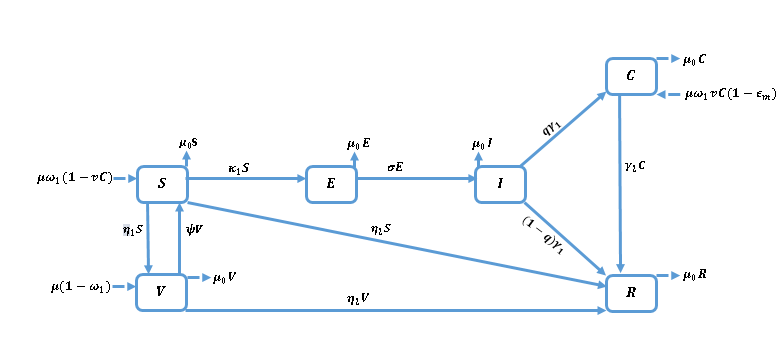
\includegraphics[scale=0.75]{infant_vaccination_model}
	\caption{the model structure indicating vertical transmission and two stages of immunity, the first through the birth vaccine, and final through a sort of booster by routine vaccination. The solid arrows indicate movement of the individuals, whiles the dashed arrows represent initial inflows and deaths.} \label{fig:flowchart}
\end{figure}

The systems of ordinary differential equations representing the dynamics described above are as follows:
\begin{align}
\begin{split}
\dfrac{dS}{dt}&=\mu\omega_1(1-\nu C)-(\mu_0+\kappa_1+\eta_2+\eta_1)S+\psi V\\
\dfrac{dV}{dt}&=\mu(1-\omega_1)+\eta_1S-(\mu_0+\eta_2+\psi)V \\
\dfrac{dE}{dt}&=\kappa_1S-(\mu_0+\sigma)E \label{eqn: 1}\\
\dfrac{dI}{dt}&=\sigma E-(\mu_0+\gamma_1)I\\
\dfrac{dC}{dt}&=(1-\epsilon_m)\mu\omega_1\nu C+q\gamma_1I-(\mu_0+\gamma_2)C\\
\dfrac{dR}{dt}&=\gamma_2C+(1-q)\gamma_1I+\eta_2(S+V)-\mu_0R
\end{split}
\end{align}
The various parameters used in our model are described the following table:

\vspace{1cm}
\begin{table}[t]
	\centering
	\begin{tabular}{ |p{1.57cm}|p{12cm}| }
		\hline
		Parameter& Description \\
		\hline
		$	\mu		$    					& 				birth rate    \\
		$	\mu_0 $					     &  	 natural death rate   \\
		$\kappa_1$ 				      & 	MTCT transmission coefficient\\
		$\epsilon_m$ 			   & 	efficacy of treatment of the infected mothers\\
		$\sigma$ 						 & 	rate of progression from exposed state to acute state\\
		$\gamma_1$				   & 	rate of moving from acute infection to carrier state\\
		$\gamma_2$ 				   & 	rate of natural clearance of infection\\
		$\omega_1$					& 	proportion of infants without successful birth vaccination\\
		$\eta_1$ 						 & 	birth vaccination rate\\
		$\eta_2$ 						 &	 routine vaccination rate\\
		$\psi$								 &	 waning rate of the birth vaccine\\
		$\nu$ 								 & 	proportion of infants infected at birth\\
		$q$ 								   & 	average probability that an infant proceeds to the carrier state due to inability to clear acute infection\\
		\hline
	\end{tabular}
	\caption{Model parameters and their descriptions}
	\label{table:1}
\end{table}

\clearpage 
%\chapter{Optimal control of onchocerciasis}
\label{chp:IMP}


%%%%%%%%%%%%%%%%%%%%%%%%%%%%%%%%%%%%%%%%%%%%%%%%%%%%%%%%%%%%%%%%%%%%%%%

%\clearpage 
%\chapter{Discussion and Conclusion}
\label{chp:DISC}


%%%%%%%%%%%%%%%%%%%%%%%%%%%%%%%%%%%%%%%%%%%%%%%%%%%%%%%%%%%%%%%%%%%%%%%
\section{Discussion}

\section{Conclusion}
%\clearpage
%%\chapter{Pricing Exotic Options and Model Risk }
%\label{C6}
% This chapter focuses on exotic options, and model risk. Model risk arises when the "wrong" financial models are applied to price financial derivatives. The statistician GEP Box wrote "All models are wrong, but some are useful" (Box, \cite{Box}, pg. $424$). In finance the  models can be "wrong"  when the numerical methods are not stable, or when the  calibration methods are incorrect.  The model risk may occur when the model prices used to compute the financial derivatives are inappropriate, and  may also be because of an inexact (or a reasonable) method  for the hedging of the derivative. Even if there is a method, we may choose the wrong one. In this chapter, we focus on the risks involved when we price exotic options. We will pay limited attention to the risks that arise from calibration to  market prices, because we have already considered the risk-neutral parameters  obtained  with the calibration of "CGMY-world" data (see chapter \ref{cp} for more details). Here, we compute a measure of model risk of call options and exotic options using the new parameters.
% 
%This chapter is organised as follows: First, we discuss the procedure of pricing exotic options and the results. We then discuss the Monte Carlo method. Finally, we compute a measure of model risk of exotic options using an improvement of the model risk formula introduced by Cont \cite{CONT}.
%
%\section{Pricing Exotic options}
%
%Exotic options have prices that are not quoted on the open market. Therefore, risk-neutral parameters calibrated to the observed market prices are needed in order to compute exotic option prices. Exotic options may be  path-dependent options, which means that their terminal values (at expiration or exercise) depends on the values of the underlier, not only at that exact time, but also at   prior points to that \cite{Link3}. We note that the application of different models calibrated to market prices can lead to different values, which happens regularly in exotic options such as lookback and barrier options.
%\subsection{Pricing Barrier Option}
%The barrier option is one of the simplest types of path-dependent option  where the holder has the right to buy or sell the underlying asset at  any specific price when the  contract expires. The important  feature about a barrier option is that its payoff does not only depend on the last (final) price of underlying asset but also on  whether or not the underlying asset may reach some level of H  (the barrier level) during the lifetime of the option (Kyprianou, Schoutens and Wilmott \cite{KAW}). The barrier may consist  of more than two barriers,  but here we focus on those with one barrier with an option payoff, up-and-in, or up-and-out calls, which we discuss in the next section.
%
%% The attraction of barrier options is that they are cheaper than the corresponding vanilla option, and also the sum of the two barriers, the Up-and in call and Up-and out call, are always  equal to the vanilla option if there is no rebate (Andreas,Schoutens and Wilmott \cite{KAW}).
%\subsubsection{ Up-and-in call}
%Let $K$ be a strike price and $H$ a barrier level. The payoff of an up-and-in call with $K$ and $H$ is equal to the payoff of a standard European call, provided that if the maximum of the underlying asset reaches (or crosses) (between the time $t\in [0,T]$) the  barrier $H$ at time $t$, while otherwise it is zero. We define the price of an up-and-in call as an expectation under the risk neutral measure $Q$ of the discounted payoff:  
%\begin{align}
%C^{UI}= \mathbb{E}_{\mathbb{Q}}[e^{-rT}(S_T-K)^+ 1_{M_T \geq H}]
%\end{align}
%where $M_T$ represents the maximum of the underlying asset $(S_t)_{t \in [0,T]}$. i.e.
%\begin{align*}
%M_t =\sup \lbrace S_u; 0 \leq u \leq t  \rbrace,
%\end{align*}
% and $r$ is an interest rate.
%%and 
%%\begin{align*}
%%(S_T-K)^+= \max(S_T-K,0).
%%\end{align*}
%We note that the value of the standard European call and the up-and-in call can be the same, if the  barrier level $H$ is lower than the strike price $K$ (i.e. $H \leq K$). If $S_T-K >0$, this means that the barrier $H \leq K$ has been crossed before the expiry time $T$.
%
%\subsubsection{Up-and-out call}  
%
%Like the price of an up-and-in call, the price of an up-and-out call is equal to the standard European call price with strike $K$, if the maximum of the underlying asset at time $t \in [0,T]$ stays below the barrier level $H$, while  otherwise it is zero. One can define the value of an up-and-out call:
%\begin{align}
%C^{UO}= \mathbb{E}_{\mathbb{Q}}[e^{-rT}(S_T-K)^+ 1_{M_T < H}].
%\end{align}
%
%As mentioned previously, when we sum both barriers up-and-in call, and up-and-out call which is called in-out parity with the same maturity $T$ and strike $K$ for any given asset price, we obtain
%
%\begin{align}
%C^{UO}+C^{UI} &= \mathbb{E}_{\mathbb{Q}}[e^{-rT}(S_T-K)^+ 1_{M_T < H}] +  \mathbb{E}_{\mathbb{Q}}[e^{-rT}(S_T-K)^+ 1_{M_T \geq H}] \nonumber \\
%& =  e^{-rT}\mathbb{E}_{\mathbb{Q}}[(S_T-K)^+ 1_{M_T \geq H} + (S_T-K)^+ 1_{M_T < H}]  \nonumber \\
%&= e^{-rT}\mathbb{E}_{\mathbb{Q}}[(S_T-K)^+ ].
%\end{align}
%Hence, this sum is equal to the standard European call option with the strike price  $K$ and maturity $T$.  In the next section  we discuss the pricing of the lookback fixed option. 
%
%%\subsubsection{A general formula for  Up- and In call, and,  Up- and out call with Black-Scholes model}
%%Black-Scholes framework John Hull \cite{MRC} and Robert \cite{HJK} expressed the general formula of the Up-and in call and Up-and out call with strike $K$ and maturity $T$ in the following:
%%For $H>K$
%%\begin{align*}
%%C^{UI}=& S_0 \Phi(z_1)e^{-qT} -Ke^{-rT}\Phi(z_1- \sigma \sqrt{T}) - S_0e^{-qT} \Big( \frac{H}{S_0}\Big)^{2 \lambda}(\Phi(-y)- \Phi(-y_1)) \\
%%&+ Ke^{-rT} \Big( \frac{H}{S_0}\Big)^{2\lambda}(\Phi(-y_1+\sigma \sqrt{T})- \Phi(y_1+\sigma \sqrt{T}));
%%\end{align*}
%%and then the Up- and out call is the difference between the European call and Up-In call:
%%\begin{align*}
%%C^{UO}=e^{-rT}\mathbb{E}_{\mathbb{Q}}[(S_T-K)^+ ]-C^{UI}.
%%\end{align*}
%%with
%% \begin{align*}
%% \lambda &= \frac{1}{\sigma ^2} \Big(r-q +\frac{\sigma ^2}{2} \Big) \\ 
%% y&= \frac{1}{\sigma \sqrt{T}} \log \Big( \frac{H^2}{S_0 K}\Big) + \lambda \sigma \sqrt{T},\\
%% z_1&=\frac{1}{\sigma \sqrt{T}} \log \Big( \frac{S_0}{H}\Big) + \lambda \sigma \sqrt{T},\\
%% y_1&=\frac{1}{\sigma \sqrt{T}} \log \Big( \frac{H}{S_0}\Big) + \lambda \sigma \sqrt{T}.
%% \end{align*} 
%% 
%%When the barrier level $H$ lays below the strike $K$, i.e. $H \leq K$, then the above Up- and in call and Up- and out call is expressed by :
%% \begin{align*}
%% C^{UI}&=e^{-rT}\mathbb{E}_{\mathbb{Q}}[(S_T-K)^+ ] \\
%% & \text{and}\\
%% C^{UO}&=0;
%% \end{align*}
%
% \subsection{Pricing the Lookback Fixed Option}
%A lookback option is a path-dependent option where the payoff depends on the  minimum or maximum  price of the underlying asset during the life of an option.  The holder of the lookback  option  may  "look back" over the period to determine the payoff. More detail about lookback option can be found in the  literature of Kyprianou, Schoutens and Wilmott \cite{KAW},  Ngugen-Ngoc \cite{NEX} and E Shreve \cite{SCF}.  There are two types of lookback option, the floating strike lookback option and the fixed strike lookback options, but here we focus on the lookback fixed option only. 
% \subsubsection{ Lookback fixed option}
%The payoff of a lookback fixed option is only dependent on the maximum of underlying asset and the strike price (or the difference between the maximum of underlying asset and the strike price during the lifetime of the option). The lookback fixed option is a type of path-dependent option that is only settled in cash, with the strike only being predetermined at inception \cite{Link}. The lookback price formula is given by:
%\begin{align}
%C_{fixed}(S_T,K,T)=e^{-rT}\mathbb{E}_{\mathbb{Q}}[(\max_{0\leq t \leq T}S_t-K,0)]
%\end{align}
%where $(S_t)_{t\in [0,T]}$ is an underlying asset, $r$ an interest rate and $K$ the strike. The  lookback option is more expensive than the similar plain vanilla option.  
%
%Having discussed lookback fixed options, we need to find the distribution of the maximum of the underlying asset process for them. The  explicit form for the distribution of maximum of a general exponential L\'evy model is often unknown.  Thus, a numerical technique is needed, such as Monte Carlo simulation, to compute the value of an exotic option (Kyprianou \cite{KAW}), and we discuss this in the next section. 
%\subsection{Monte Carlo Method}
%%The main purpose for choosing the Monte Carlo method is that we can easily price the derivative security, particularly the  European and exotic options, without knowing their explicit form in relation to general L\'evy model.  The Monte Carlo method is a numerical method, which is used  to perform computations using the function of the random variable (Schoutens \cite{WS}). Thus, this method takes  the average value and runs a sequence experiment.  When writing an expectation of payoff under the integral form, we note that the dimension of its integral can be infinite, hence the importance of using the Monte Carlo method.  In order to calculate the derivative security, first ,you simulate the paths of the underlying asset price using the model calibrated. To obtain an accurate result from Monte Carlo method, we either need to simulate a large number of paths or use proposed technique such as the antithetic variable and control variable technique, which allows us to reduce  the variance of the simulation estimate. 
%
%Schoutens \cite{WS} highlighted that the  value of the standard error obtained by simulating a large  number of paths without using the variance reduction method may be similar to those obtained via the simulation of the paths of the underlying asset based on the variance reduction method for an exotic option. To check the accuracy of the Monte Carlo simulation we  price the European calls using $50\;000$ paths of the underlying asset for each model based on single parameters calibrated to S$\&$P 500 index option call. Figure \ref{F} shows that pricing the European call option using the CGMY, NIG, BS and VG models gives very satisfactory results. With respect to their analytic calibration values, prices values differed less than $0.2\%$ among the  pure jump models and $30\%$ using the Black-Scholes model. Thus, we computed the above lookback fixed option and barrier option using $50\;000$ paths of the underlying asset  for each model. We outline how to compute the Monte Carlo method for an exponential L\'evy model as follows (Glassernam \cite{MCM} and Hull \cite{HJK}):
% \begin{itemize}
% \item[1] Estimate  the risk-neutral parameters using  an optimization procedure (minimizing error between the observed plain vanilla  S$\&P$500 index data with model price ). This was done in chapter \ref{cp}. 
% \item [2] Use the risk-neutral parameters obtained via procedure $(1)$ to simulate the $N$ paths (trajectories) of the underlying asset for each model price. This procedure is carried out in section \ref{S}.
% \item[3] Compute the value of payoff $ ( P_j)_{1 \leq j \leq N} $  for each of the trajectories of the underlying asset.
% \item[4] Estimate the expected payoff of $P$ by taking the mean of the payoff $P_j$, denoted: 
% \begin{align*}
% P =\frac{1}{N}\sum_{j=1}^N P_j
% \end{align*}
% \item[5] We discount:% with respect to the interest rate $r$ so that we obtain the price of derivative security:
% \begin{align*}
% D= e^{-rT}P.
% \end{align*}
% \end{itemize}
% In Appendix we present methods for the simulation of  the trajectories of the pure jump L\'evy model using  Monte Carlo method.
%\begin{figure}[h!]
%\centering
%  \begin{tabular}{@{}cccc@{}}
%    \includegraphics[width=0.6 \textwidth,  natwidth=610,natheight=642]{../Pricing_Barrier/MC_C.png}    &
%  \end{tabular}
%  \caption{ The vanilla call prices computed with CGMY, NIG and VG models using the Monte Carlo method with the strike price $K=1130$, maturity $T = 0.67123$ and the stock price $S0 = 1124.47$.  } \label{F}
%\end{figure}
%
%\section{Results and Discussion}
%%Table shows the European call price computed via Monte Carlo method for each model prices. One can easily see that the European call price obtain with NIG model , VG model, CGMY model and Black Scholes model  are very  closed to the observed European call from $2002$. This means those the Monte Carlo method give a very aceptable result. 
%%In this section, we want to compute the price of  the lookback fixed option and the barrier option for the  NIG model, VG model, CGMY model and  Black scholes model as well. The single model parameters use to price those several exotic options are obtained via the calibration of S\&P 500 indexed option described in chapter\ref{cp}. We first discuss the accuracy of the Monte Carlo method. Table1 displays the results of the European call price computed via Monte Carlo method for the single risk neutral parameters for our given model prices.  One can easily see that the European call price obtained from the NIG model, VG model, CGMY model and Black Scholes model are very closed to the observed European call from December $2002$ of S\&P 500 indexed option. Therefore, we can say that the Monte Carlo method give a very satisfactory results. We now turn our attention to the results of the exotic option. 
%
%%In this section, we want first to discuss the accuracy of Monte Carlo simulation and then next use this simulation technique in order to compute the price of  the lookback fixed option and the barrier option for those model prices such as the  NIG model, VG model, CGMY model and  Black scholes model as well. We use the model parameters obtained via the calibration of the S\&P 500 indexed option from December $2002$ described in Chapter\ref{cp}, in order to price a plain vanilla European call and the several exotic options. Table1 displays the results of the European call price computed via Monte Carlo method for each model prices.  One can easily see that the plain vanilla European call  obtained from the NIG model, VG model, CGMY model and Black Scholes model are very closed to the observed European call from December $2002$ of the S\&P 500 indexed option. Therefore, we can say that the Monte Carlo simulation give a very good results. We now turn our attention to the results of the exotic option. 
%In this section, we compare the prices of the barrier and lookback options computed with all models (Black-Scholes model, NIG, VG and CGMY models) and discussed it. We consider the multiple parameters calibrated to the S$\&P$500 index data (see Chapter \ref{ch5}, Table \ref{AD1}) to value the exotic options.  We compute the exotic option prices using the Monte Carlo method discussed above. We use the maturity from December $2002$ ($T=0.6543$).  The  barrier level is a function of the stock price (ranging from $0.5(S_0)$  to $1.5(S_0)$). We simulate $50\;000$ underlying assets for each model.
%\begin{table}[h!]
%\begin{center}
%   \caption{Here we report the results of the barrier and lookback fixed options for each model price. The barrier level ranges from $(0.5s_0 to 1.5S_0)$ and the strike price $K=1130$, maturity $T = 0.67123$ and the stock price $S_0 = 1124.47$.}
%    \begin{tabular}{| l|l | l | l |p{3cm}|}
%    \hline
%   Exotic options &  CGMY model & NIG model & VG model &BS \\ \hline
% Lookback fixed &  115.5749  & 100.0157 &    96.1811 &  129.5181 \\ \hline  
% \hline
% 
% Barrier level&  Up-In \&  Up-out &Up-In \&  Up-out   &Up-In \& Up-out & Up-In \&  Up-out \\ \hline 
%Up-out+Up-In&  61.8570  & 64.1673 &  64.0775  & 68.4472 \\ \hline  
% \multirow{6}{*}{} &  & & & \\
%  562.2&  61.8570 \& 0.000 &  64.1673 \& 0.000 &    64.0775\& 0.000  &68.4472 \& 0.000  \\
% 618.5&  61.8570\& 0.000 &   64.1673 \& 0.000  &64.0775\& 0.000  &   68.4472 \& 0.000  \\
%674.7&   61.8570 \& 0.000&  64.1673 \& 0.000   &64.0775\& 0.000 &   68.4472 \& 0.000  \\ 
%   730.9 &  61.8570 \& 0.000 &  64.1673 \& 0.000  &64.0775\& 0.000  &  68.4472 \& 0.000  \\
% 787.1 &  61.8570 \& 0.000 &   64.1673 \& 0.000  & 64.0775\& 0.000 &  68.4472 \& 0.000  \\
% 843.4 &   61.8570 \& 0.000&  64.1673 \& 0.000  & 64.0775\& 0.000 &   68.4472 \& 0.000 \\ 
% 899.6   &  61.8570 \& 0.000 &  64.1673 \& 0.000  & 64.0775\& 0.000  &  68.4472 \& 0.000  \\
%955.8 &  61.8570 \& 0.000 &  64.1673 \& 0.000  & 64.0775\& 0.000  &   68.4472 \& 0.000  \\
% 1012.0 &   61.8570 \& 0.000&  64.1673 \& 0.000  & 64.0775\& 0.000  &   68.4472 \& 0.000 \\
%  1068.2   &  61.8570 \& 0.000 &  64.1673 \& 0.000  & 64.0775\& 0.000   &   68.4472 \& 0.000  \\
% 1124.5 &  61.8570 \& 0.000 &  64.1673 \& 0.000  & 64.0775\& 0.000  &   68.4472 \& 0.000  \\
% 1180.7 & 61.4715 \&  0.3855 & 62.6379 \& 1.5294   & 60.6112 \& 3.4663 & 68.1589 \&    0.2883 \\
%   1236.9  & 57.3557 \&   4.5013  &   53.4172 \& 10.7501 &  48.5999 \& 15.4776 &   65.1845 \&    3.2627   \\
%1293.1  &  47.7503 \& 14.1066& 37.0613 \& 27.1060    &   32.2969 \&   31.7806 &   57.4158 \&   11.0315 \\
% 1349.4 & 34.9839 \& 26.8731 & 22.4209 \&    41.7464   &    19.2353 \& 44.8423 &    46.0650 \&  22.3822   \\ 
%  1405.6   &22.8381   \&    39.0189 & 12.3669 \&  51.8004 &       11.3951 \& 52.6825 & 
%33.2846 \&    35.1626  \\
% 1461.8 &   13.7196   \&  48.1374    &   6.5848 \&    57.5825 & 6.6119 \& 57.4656 &
%   22.2415  \& 46.2058 \\
%  1518.0 &  7.4452   \& 54.4117 & 3.6124 \& 60.5549  &  3.8153  \&  60.2622  & 14.1877 \& 54.2595  \\ 
%  1574.3   &3.7853      \& 58.0716 & 1.7984 \& 62.3689   &   2.1468  \&  61.9307 &   8.3660 \&   60.0812  \\
%1630.5 & 1.8640\& 59.9930  &  0.9429 \&   63.2244 &  1.2145 \&  62.8630 &   4.7021
% \& 63.7451   \\
% 1686.5 &  0.9189   \& 60.9380 &  0.4400 \&    63.7273 &   0.8094 \&   63.2681  &  2.5324 \& 65.9148\\ \hline
%    \end{tabular}\label{AD4}
%\end{center}
%\end{table}
%\begin{figure}[h!]
%\centering
%  \begin{tabular}{@{}cccc@{}}
%    \includegraphics[width=0.5 \textwidth,  natwidth=610,natheight=642]{../Pricing_Barrier/PR.png}    &
%    \includegraphics[width=0.5 \textwidth,  natwidth=610,natheight=642]{../Pricing_Barrier/PR1.png}  & 
%  \end{tabular}
%  \caption{ The figures of up-and-in and up-and-out calls for NIG, VG, CGMY  and Black-Scholes models, with the strike price $K=1130$, maturity $T = 0.67123$ and the stock price $S0 = 1124.47$. The barrier level is range from $(0.5 S0$ to $1.5S0)$ } \label{ff1}
%\end{figure}
%%%%%%%%%%%%%%%%%%%%%%%%%%%%%%%%%%%%%%%%%%%%%%%%
%In Table \ref{AD4} we present the results of the barrier and lookback fixed options computed with CGMY, NIG, VG and Black-Scholes models. We observe that the sum of the values of the up-and-in call and up-and-out call options substantiate the identity of the \textit{(Up-and-In)+ (Up-and-Out)= plain vanilla}. %This means that the simulation results are well converged \cite{APC}.
%
%
%Table \ref{AD4}, as well as Figure \ref{ff1}  show that the values of the up-and-in and up-and-out call obtained with the NIG, and VG models are very similar but they differ from the values  obtained from the CGMY and Black-Scholes models. The up-and-in and up-and-out call computed using the Black-Scholes model are larger than those obtained using the NIG, VG and CGMY models. Since the "true" or "real" prices of the exotic options are unknown, it is difficult to judge which model gives the best price for the barrier option.
%  %Thus, we can say that the Black-Scholes model overpriced the prices of the Up- and-In and up-and-out call compare to the VG, NIG and CGMY models. We also observe that the NIG and VG models give a better estimation of the prices of  up-and-in and up-and-out call compared to the  to the CGMY model. Despite the fact that the CGMY model fits well the observed markets (see table \ref{AD1}). 
% 
%Similarly, the prices of the lookback fixed option computed with the VG, NIG, CGMY and Black-Scholes models are  different to each other. Once again the price of a lookback option computed with the Black-Scholes model is larger than the prices of lookback option computed using the NIG, VG and CGMY models. In addition, the prices of the lookback option computed with the NIG and VG models differ slightly, while the price obtained with the CGMY model differs from those of the  NIG, VG and Black-Scholes models. Hence, the situation is comparable to that of the up-and-in and up-and-out calls, as it is difficult to tell which model prices the exotic option best as the "true" prices of the exotic options are unknown. Therefore, in next the section, we use the exotic prices computed with the CGMY model (using the varying parameters of CGMY model see Chapter \ref{ch5}, Section \ref{s}) as our "true" prices and compare the prices of the exotic options obtained from the VG, NIG and Black-Scholes models against these prices.  
% 
% %Up-and-In and up-and-out call obtained with the NIG, VG and CGMY models are very similar while  the one obtained with the Black-Scholes model are very different and larger. We can say that Black-Scholes model model overprice the value of the Up- and-In and up-and-out call.
%
%%In other hand we observed that the prices of the  lookback fixed option computed with those models (VG, NIG, CGMY and Black-Scholes models) are  different to each other.  Once again we found that  Black-Scholes model gives very large price of the  price for the lookback fixed option compare to the lookback fixed prices computed via NIG, VG and CGMY models. Based on these results we say that the  NIG, VG and CGMY models give the very similar values for the prices of  the Up-in and Up-Out call and different values for the lookback fixed option. While the  Black-Scholes model overprice both  Up-in and Up-Out call and the lookback fixed option compare to the NIG, VG and CGMY models. 
%
% %We can also  see that the values of Up-in and Up -out obtained with the NIG, VG and CGMY models are very similar, while  they differ a little bite with the  one obtained from Black-Schloes model. However, when  we look at the value of the lookback fixed option computed with those models (VG, NIG, CGMY and Black-Scholes models) are  different to each other. We can see that the value of lookback fixed option computed with the CGMY model is larger than the values obtained with the  NIG, VG and Black-Scholes models. Based on these results, we can say that the  NIG, VG and CGMY models give the similar values when we price the Up-in and Up-Out, and the different values for the case of the lookback fixed option. 
%
%%In next section, we will compute the model risk for the exotic options. 
% 
% %When we look at on this table1, one can easily that the results for the  Up-In call and Up-Out call computed via the CGMY model, NIG model and also VG model are very similar, while the one obtained from the Black-Scholes model differ a little bite. The same scenario repeats for the Lookback fixed option. This does not mean that the the Black-Scholes model (BSM ) still misprice the exotic option. However, it will be more important to compute the model risk for those exotic options. The reason that we are computing the model risk is that we are looking for a good model which can present less risk in pricing the exotic options.
% 
% 
%% From Table 1 shows the results from CGMY process, NIG process , VG process and Black %Scholes model as well. We can see that the results for the barrier option verify well the identity $Up-In+Up-Out= plain Vanilla $. This means that the results are well converged. When we look at the table below, one can easily that the results for the  Up-In call and Up-Out call from CGMY process, NIG process and VG process are very similar, while the one from the Black Scholes model differ a little bite.  The same scenario repeats for the Lookback fixed option which is presented in same table. This means that the Black Scholes model (BSM ) still misprice the exotic option. But, it  does not mean that the Black-Scholes model present more risk  in pricing exotic than  the remain model such as NIG, VG and CGMY model as well.  It will be more useful to compute the model risk for those exotic options so that we can  know which amongst four models may present less risk in pricing exotic. This will be an object for the next section . 
%\section{ Model risk}\label{MR}
%
%%Comparing the pricing of the exotic options obtain with CGMY model against the one obtain with the NIG, VG and Black-Scholes models and
%In the previous section  we found it difficult to justify which of four models produced the best price for an exotic options, since the "true" prices were unknown. Here, we price both of exotic options (barrier and lookback options) with the CGMY model using its varying parameters (the parameters obtained by increasing and decreasing the multiple parameters of CGMY model as described in Section \ref{s}), and we consider those  prices as our "true" exotic prices. The aim here is to check which of the four models can price the exotic options best when we compare their prices to the "true" prices obtained with the CGMY model. To price the exotic options with NIG, VG and Black-Scholes models, we consider their risk-neutral parameters calibrated to "CGMY-world" data (i.e. the market prices computed with the CGMY model using its varying parameters). We use the Monte Carlo method to compute the price of the up-and-in, up-and-out calls and the lookback options. We simulate $50\;000$ paths of the underlying assets for each model. We consider  the strike price when the option is out-of-the-money and in-the-money $K = 110$  and $95$ respectively, the spot price $100$, the interest rate at $r=0.019$, the dividend yield at $q=0.012$ and one year of maturity $T=1$. We assume that a year consists of $250$ trading days. The barrier level is a function of the initial stock price (ranging from $1S0 $ to $1.5S0 $). Below we compare the prices of the barrier and lookback options both  when the option prices are in-the-money and out-the-money and computed with all models. We start by comparing the prices of the barrier and lookback option when the option is out-of-the-money, (i.e. $K=110>S_0=100$).
%
% %We recall that  the new parameters of the NIG, VG and Black-Scholes models  are calibrated from the  market data computed with the varying model model parameters of the CGMY model (see tables \ref{A1}, \ref{A1i} and \ref{A2}).
%
% 
%
%
%Figures \ref{fji}, \ref{fj4}, \ref{fj1}, \ref{fj2}  and \ref{fj3}  show the results of the comparison for the barrier prices of the up-and-in call computed with the various sets of the new parameters of the CGMY, NIG, VG and BS models between the "true" prices of the up-and-in call (i.e. prices computed with CGMY model using its varying parameters sets) when the option is out-the-money.\\
%\begin{figure}[!htbp]
%\centering
%  \begin{tabular}{@{}cccc@{}}
%    \includegraphics[width=0.5 \textwidth,  natwidth=610,natheight=642]{../Pricing_Barrier/FC5.png}    & 
%        \includegraphics[width=0.5 \textwidth,  natwidth=610,natheight=642]{../Pricing_Barrier/FC8.png}   & \\
%            \includegraphics[width=0.5 \textwidth,  natwidth=610,natheight=642]{../Pricing_Barrier/FC6.png}  & 
%  \end{tabular}
%  \caption{ We computed the prices of the  up-and-in and up-and-out for NIG, VG, CGMY and BS models obtained with the  model parameters calibrated  from the vanilla call computed with the  model parameters (C$^+$,G,M,Y$^-$), (C,G,M,Y$^-$) and (C$^+$, G, M, Y $^+$). The barrier level ranges from $1(S_0 )$ to $1.5(S_0 )$, the strike price is  $K = 110$, the spot price is equal $S0=100$, the risk-interest rate $r=19 \%$, dividend yield at $q=12\%$  and maturity $T=1$}\label{fji}
%\end{figure}
%\begin{figure}[!htbp]
%\centering
%  \begin{tabular}{@{}cccc@{}}
%       \includegraphics[width=0.5 \textwidth,  natwidth=610,natheight=642]{../Pricing_Barrier/FC7.png}  &
%    \includegraphics[width=0.5 \textwidth,  natwidth=610,natheight=642]{../Pricing_Barrier/FC2.png}   & 
%%    \includegraphics[width=0.5 \textwidth,  natwidth=610,natheight=642]{../Pricing_Barrier/F_c4.png}   &
%    
%  \end{tabular}
%  \caption{ We computed the prices of the up-and-in and up-and-out for NIG, VG, CGMY and BS models obtained with the model parameters calibrated  from the vanilla call computed with the  model parameters (C, G, M, Y$^+$) and (C$^+$, G, M, Y ). The barrier level ranges from $1S0 $ to $1.5S0 $, the strike price is  $K = 110$, the spot price is equal $S_0=100$, the riskless $r=19\%$, dividend yield  $q=12\%$  and maturity $T=1$} \label{fj4}
%\end{figure}
%
%\begin{figure}[!htbp]
%\centering
%  \begin{tabular}{@{}cccc@{}}
%    \includegraphics[width=0.5 \textwidth,  natwidth=610,natheight=642]{../Pricing_Barrier/FC3.png}  &
% %   \includegraphics[width=0.5 \textwidth,  natwidth=610,natheight=642]{../Pricing_Barrier/F_ou.png}   & 
%  \end{tabular}
%  \caption{ We computed the prices of the up-and-in and up-and-out NIG, VG, CGMY and BS models obtained with the  model parameters calibrated  from the vanilla call computed with the  model parameters. (C $^-$, G, M, Y $^-$).  The barrier level ranges from $1S0 $ to $1.5S0 $, the strike price is  $K = 110$, the spot price is equal $S_0=100$, the risk-interest rate $r=19\%$, dividend yield  $q=12 \%$  and maturity $T= 1$} \label{fj1}
%\end{figure}
%%
%\begin{figure}[!htbp]
%\centering
%  \begin{tabular}{@{}cccc@{}}
%    \includegraphics[width=0.5 \textwidth, natwidth=610,natheight=642]{../Pricing_Barrier/FC4.png}    &
%    \includegraphics[width=0.5 \textwidth,  natwidth=610,natheight=642]{../Pricing_Barrier/FC1.png}    & \\
%%     \includegraphics[width=0.5 \textwidth,  natwidth=610,natheight=642]{../Pricing_Barrier/F_in3.png}   &
%%   \includegraphics[width=0.5 \textwidth,  natwidth=610,natheight=642]{../Pricing_Barrier/F_ou3.png}   & 
%    
%  \end{tabular}
%  \caption{ We computed the prices of the up-and-in and up-and-out for NIG, VG, CGMY and BS models obtained with the  model parameters calibrated  from the vanilla call computed with the  model parameters (C$^-$,G,M,Y$^+$) and  (C$^-$,G,M,Y ).  The barrier level ranges from $1S0 $ to $1.5S0 $, the strike price is  $K = 110$, the spot price is equal $S_0=100$, the risk-interest rate $r=19 \%$, dividend $q=12\%$  and maturity $T=1$} \label{fj2}
%\end{figure}
%
%
%\begin{figure}[!htbp]
%\centering
%  \begin{tabular}{@{}cccc@{}}
%    \includegraphics[width=0.5 \textwidth,  natwidth=610,natheight=642]{../Pricing_Barrier/FC.png} &
%%    \includegraphics[width=0.5 \textwidth,  natwidth=610,natheight=642]{../Pricing_Barrier/F_ou4.png}   & \\
%  \end{tabular}
%  \caption{ We computed the prices of the up-and-in and up-and-out for NIG, VG, CGMY and BS models obtained with the  model parameters calibrated  from vanilla calls computed with the  model parameters (C,G,M,Y).  The barrier level ranges from $1S0 $ to $1.5S0 $, the strike price is  $K = 110$, the spot price is equal $S0=100$, the riskless $r=19 \%$, dividend yield $q=12 \%$  and maturity $T=1$} \label{fj3}
%\end{figure}
%
%The aforementioned figures also show that the prices of barrier options computed with the various sets of the new parameters differ from each other. This is to be expected since different sets of the parameters may lead to the different exotic options prices. If the barrier level is equal to the spot price (i.e. the value of the up-and-in calls =vanilla calls), we see in the Figure \ref{fji}  that the prices of the up-and-in calls computed with the BS model are larger than our current "true" prices while the prices of the up-and-in calls obtained with the NIG and VG models are smaller than current "true" prices. In the paper of  Schoutens \cite{WSC}, he shows that the difference between barrier option prices computed across models may be as much as $200 \%$. Similarly, here we notice that the  percentage error between the values of the up-and-in calls  obtained between the BS prices and "true" prices  with new parameters calibrated to "CGMY-world" data obtained from the following varying sets ((C$^+$,G,M,Y$^-$), (C,G,M,Y$^-$), (C$^+$,G,M,Y$^+$)) are $40 \%,79 \%, 12 \%$  and the ones obtained with NIG and VG models are  $57 \%, 8 \%, 31 \%$ and $58 \%, 30 \%, 54 \%$. This suggests evidence of the model risk. For example. the BS model overprices the prices of the up-and-in call, as is illustrated by the percentage error between the BS and the "true" price of the up-and-in calls of $79 \% $, while the percentage error between the  prices of up-and-in call obtained with  VG and NIG models is up to $30 \% $ and $8 \% $. Here it is clear that BS model is an inappropriate model because of its poor calibration. In addition, the percentage error between the prices of the up-and-in calls computed with CGMY model  with all set of the new parameters and our current "true" prices are ($-2.81\%, 1.28\%, 5.7\%, -0.04\%, -2.62\%, -3.75\%, -0.02\%, -2.45\%, -26.44\%$) which differs from zero,  despite the fact that these new parameters are calibrated to "CGMY-world" data. We expected this since we observed a slight difference between the new parameters of CGMY model and its varying parameters (see Section \ref{Sub}).
%
% That means the prices of the up-and-in calls are very sensitive to calibration risk, and also that calibration risk can be seen as a cause of model risk.
%
%
%
%% since its prices are larger than our current "true" prices.
%%Thus, if one wants to price the up-and-in call considered the BS model instead the VG and NIG models with the new parameters calibrated to "CGMY-world" data  obtained with the different varying parameters sets (C$+\Delta =20\%C$,G,M,Y^+), (C^+,G,M,Y$-\Delta =20\%C$ ) and (C,G,M,Y^-), can be exposed to model risk.
% 
%In Figures \ref{fj2}, \ref{fj3} and \ref{fj4}, we show that the prices of the up-and-in call computed with BS model with the new parameters calibrated to "CGMY-world" data obtained with  varying parameters set ((C$^-$,G,M,Y ), (C$^-$,G,M,Y$^+$),(C$^+$,G,M,Y$^-$), (C,G,M,Y$^+$) and (C,G,M,Y)) are similar to "true" prices while the ones obtained with the NIG and VG model are  different to current "true" prices. Thus by pricing up-and-in calls with NIG and VG models, we are exposed to model risk as there are huge differences between the "true" price of the up-and-in call and the ones obtained with NIG and VG models $(48 \%, 69 \%, 70\%, 68\%, 78\%$ and $55\%, 84\%, 85\%, 88\%, 92\%$ respectively), despite the fact that NIG and VG models fit the "CGMY-world" data better than BS model. In contrast, the percentage error between the "true" price of the up-and-in call and the ones obtained with BS model are only $0.35\%, 2\%, 9\%, 15\%, 25\%$.  %We  still observe that the difference between the CGMY prices and our the "true" price of the up-and-in calls $(111)$  are not close to zeros.  
%Once again, we agree with Schoutens \cite{WSC} that the difference of the barrier between model may be up to $(200\%)$.
%
%Finally, in Figure \ref{fj1}, we show that the price of up-and-in call computed with the NIG model using the new parameters calibrated to "CGMY-world" data obtained with the varying parameters set (C$^-$,G,M,Y$^-$ ) are close to "true" prices while the ones obtained with the VG and BS models differ to current "true" prices, despite the fact that VG and NIG model have a same number of risk-neutral parameters and also fit the "CGMY-world" data better than BS model. The difference between the up-and-in call obtained with NIG model and "true" prices is up $(20\%)$ while the ones between the VG and BS models and "true" prices are $100\%$ and $94\%$. 
%
%Furthermore, we note that when the option is out-the-money, it is difficult to avoid model risk when we price the barrier (especially the up-and-in call) since any model carries model risk. We observed that the percentage error between the up-and-in calls obtained with NIG, VG and BS  models and our current "true" price may be as much as $100\%$.
%
%%%%%%%%%%%%%%%%%%%%%%%%%%%%%%%%%%%%%%%%%%%%%%%%%%%%%%%%%%%%%%%%%%%%%%%%%%%%
%\begin{table}[!htbp]
% \begin{center}
%   \caption{The price values of the lookback options computed with all different model parameters. Strike price $K=110$, spot price  $S_0=100$, interest rate $r=19 \%$, dividend yield $q=12\%$ and $T=1$ }
%        \setlength{\arrayrulewidth}{0.5mm}
%\setlength{\tabcolsep}{8pt}
%\renewcommand{\arraystretch}{1.5}
%\newcolumntype{s}{>{\columncolor[HTML]{AAACED}} p{3cm}}
%
%\arrayrulecolor[HTML]{DB5800}
%\begin{tabular}{|p{6cm}|p{1cm}|p{1cm}|p{1cm}|p{1cm}|p{1cm}|}
%\hline 
% CGMY, NIG, VG and BS  parameters calibrated to "CGMY-world" data obtained with  the following set of varying parameters  & "True" prices & CGMY prices & NIG prices & VG prices & BS prices \\ 
%\hline 
% (C, G, M, Y) &  6.5663 & 6.5332 &  5.2227 & 4.9078 &  7.8403 \\ 
%\hline 
%  (C$^-$, G, M, Y) & 4.9122 & 4.8593 & 3.9355 & 3.5030 &6.2116 \\ 
%\hline                                 
% (C$^+$, G, M, Y) & 7.7543 & 7.6380 & 6.5446 &  6.2431 &9.4155 \\ 
%\hline 
% (C$^-$, G, M, Y$^-$) &  1.2443 & 1.2608 & 1.3921 & 2.2502 &3.4343 \\ 
%\hline 
% (C$^-$, G, M, Y$^+$) & 5.0595 & 5.0886 & 4.0304  &3.7204 &6.3973 \\ 
%\hline 
% (C$^+$, G, M, Y$^-$) &  3.5190 & 3.5420 & 2.8348 & 2.6430  & 6.2116 \\ 
%\hline 
% (C$^+$, G, M, Y$^+$) & 7.8084 & 7.7701& 6.7779 &6.2489 &9.5461 \\ 
%\hline 
% (C, G, M, Y$^-$) &2.3022 & 2.3090 & 2.1477 &  1.7673 & 4.7501 \\ 
%\hline 
% (C, G, M, Y$^+$) & 6.6417 & 7.5967 & 5.3596 & 5.0049 &8.2665 \\ 
%\hline
%\end{tabular}\label{Ai1}
%\end{center}
%\end{table}
%
%
%%%%%%%%%%%%%%%%%%%%%%%%%%%%%%%%%%%%%%%%%%%%%%%%%%%%%%%%%%%
%
%%\begin{table}[!htbp]
%% \begin{center}
%%   \caption{The price value of the lookback fixed computed with all different model parameters. Strike price $K=110$, spot price  $S_0=100$, interest rate $r=19 \%$, dividend $q=12\%$ and $T=1$ }
%%     \setlength{\arrayrulewidth}{0.5mm}
%%\setlength{\tabcolsep}{8pt}
%%\renewcommand{\arraystretch}{1.5}
%%\newcolumntype{s}{>{\columncolor[HTML]{AAACED}} p{3cm}}
%%
%% 
%%\arrayrulecolor[HTML]{DB5800}
%%%{\rowcolors{3}{green!80!yellow!50}{green!70!yellow!40}
%%\begin{tabular}{|p{1cm}|p{1cm}|p{1cm}|p{1cm}|l}
%%\cline{1-4}
%%\multicolumn{4}{ |c| }{The lookback fixed computed with all model parameters far all models }  \\ \cline{1-4}
%%%\rowcolor{green!80!yellow!50} 
%%CGMY-lookback fixed & NIG-lookback fixed & VG-lookback fixed & BS-lookback fixed\\ \cline{1-4}
%%\multicolumn{4}{|p{16cm}| }{  The results of the price of the lookback  presented below are computed with the new parameters ( NIG, VG and BS models)  calibrated  with the "CGMY-world" data computed via the set of the varying parameters $(C=0.0332, G=0.4614, M=15.6995, Y=1.2882)$} \\ \cline{1-4}
%%\multicolumn{1}{ |c  }{ 6.5663 }                        &
%%\multicolumn{1}{ |c| }{  5.2227}&   4.9078 &    7.8403 &  \\ \cline{1-4}
%%          \multicolumn{4}{|p{16cm}| }{  The results of the price of the lookback presented below are computed with the new parameters ( NIG, VG and BS models)  calibrated  with the "CGMY-world" data computed via the set of the varying parameters $(C=0.0266, G=0.4614, M=15.6995, Y=1.2882)$} \\      
%%    \cline{1-4}
%%\multicolumn{1}{ |c  }{ 4.9122} &
%%\multicolumn{1}{ |c| }{  3.9355}&   3.5030&  6.2116&   \\ \cline{1-4}
%%\multicolumn{4}{|p{16cm}| }{  The results of the price of the lookback  presented below are computed with the new parameters ( NIG, VG and BS models)  calibrated  with the "CGMY-world" data computed via the set of the varying parameters $(C=0.0398, G=0.4614, M=15.6995, Y=1.2882)$}  \\ \cline{1-4}
%%\multicolumn{1}{ |c  }{ 7.7543 }                        &
%%\multicolumn{1}{ |c| }{ 6.5446 }&  6.2431&    9.4155 &  \\ \cline{1-4}
%%\multicolumn{4}{|p{16cm}| }{  The results of the price of the lookback  presented below are computed with the new parameters ( NIG, VG and BS models)  calibrated  with the "CGMY-world" data computed via the set of the varying parameters $(C=0.0266, G=0.4614, M=15.6995, Y=1.0306)$}   \\ \cline{1-4}
%%%%%%%%%%%%%%%%%%%%%%%%%%%%%%%%%%%%%%%%%%%%%%%%%%%%%%%%%%%%%%%%%%
%%\multicolumn{1}{ |c  }{    1.2443}                        &
%%\multicolumn{1}{ |c| }{  1.3921}&  2.2502 & 3.4343   &  \\ \cline{1-4}
%%
%%%%%%%%%%%%%%%%%%%%%%%%%%%%%%%%%%%%%%%%%%%%%%%%%%%%%%%%%%%%%%%%%%%%%%%
%%\multicolumn{4}{|p{16cm}| }{  The results of the price of the lookback  presented below are computed with the new parameters ( NIG, VG and BS models)  calibrated  with the "CGMY-world" data computed via the set of the varying parameters $(C=0.0266, G=0.4614, M=15.6995, Y=1.2948)$}  \\ \cline{1-4}
%% \multicolumn{1}{ |c  }{ 5.0595}                        &
%%\multicolumn{1}{ |c| }{  4.0304 }&   3.7204 &  6.3973 &  \\ \cline{1-4}
%%
%%\multicolumn{4}{|p{16cm}| }{  The results of the price of the lookback  presented below are computed with the new parameters ( NIG, VG and BS models)  calibrated  with the "CGMY-world" data computed via the set of the varying parameters $(C=0.0398, G=0.4614, M=15.6995, Y=1.0306)$}  \\ \cline{1-4}
%%
%%\multicolumn{1}{ |c  }{  3.5190}                        &
%%\multicolumn{1}{ |c| }{ 2.8348 }&  2.6430 & 6.2116  &  \\ \cline{1-4}
%%
%%
%%\multicolumn{4}{|p{16cm}| }{  The results of the price of the lookback  presented below are computed with the new parameters ( NIG, VG and BS models)  calibrated  with the "CGMY-world" data computed via the set of the varying parameters $(C=0.0398, G=0.4614, M=15.6995, Y=1.2948)$}    \\ \cline{1-4}
%%\multicolumn{1}{ |c }{  7.8084 }                        &
%%\multicolumn{1}{ |c| }{6.7779}&6.2489&    9.5461  & \\ \cline{1-4}
%%
%%\multicolumn{4}{|p{16cm}| }{  The results of the price of the lookback  presented below are computed with the new parameters ( NIG, VG and BS models)  calibrated  with the "CGMY-world" data computed via the set of the varying parameters $(C=0.0332, G=0.4614, M=15.6995, Y=1.0306)$}   \\ \cline{1-4}
%%
%%\multicolumn{1}{ |c  }{   2.3022}                        &
%%\multicolumn{1}{ |c| }{2.1477 }  & 1.7673& 4.7501 &   \\ \cline{1-4}
%%\multicolumn{4}{|p{16cm}| }{  The results of the price of the lookback  presented below are computed with the new parameters ( NIG, VG and BS models)  calibrated  with the "CGMY-world" data computed via the set of the varying parameters $(C=0.0332, G=0.4614, M=15.6995, Y=1.948)$}   \\ \cline{1-4}
%%\multicolumn{1}{ |c  }{6.6417}                        &
%%\multicolumn{1}{ |c| }{5.3596}  &5.0049& 8.2665 &  \\ \cline{1-4} 
%%\end{tabular}\label{Ai}
%%\end{center}
%%\end{table}
%
%
%
%
%%%%%%%%%%%%%%%%%%%%%%%%%%%%%%%%%%%%%%%%%%%%%%%%%%%%%%%%%%%%%%%%%%%%%%%%%%%%%%%%%
%%\begin{table}[!htbp]
%% \begin{center}
%%   \caption{The price value of the lookback fixed computed with all different model parameters. Strike price $K=110$, spot price  $S_0=100$, interest rate $r=19 \%$, dividend $q=12\%$ and $T=1$ }
%%     \setlength{\arrayrulewidth}{0.5mm}
%%\setlength{\tabcolsep}{8pt}
%%\renewcommand{\arraystretch}{1.5}
%%\newcolumntype{s}{>{\columncolor[HTML]{AAACED}} p{3cm}}
%%
%% 
%%\arrayrulecolor[HTML]{DB5800}
%%%{\rowcolors{3}{green!80!yellow!50}{green!70!yellow!40}
%%\begin{tabular}{|p{1cm}|p{1cm}|p{1cm}|p{1cm}|l}
%%\cline{1-4}
%%\multicolumn{4}{ |c| }{The lookback fixed computed with all model parameters far all models }  \\ \cline{1-4}
%%%\rowcolor{green!80!yellow!50} 
%%CGMY-lookback fixed & NIG-lookback fixed & VG-lookback fixed & BS-lookback fixed\\ \cline{1-4}
%%\multicolumn{4}{|p{16cm}| }{  The results of the price of the lookback  presented below are computed with the new parameters ( NIG, VG and BS models)  calibrated  with the "CGMY-world" data computed via the set of the varying parameters $(C=0.0332, G=0.4614, M=15.6995, Y=1.2882)$} \\ \cline{1-4}
%%\multicolumn{1}{ |c  }{ 6.5663 }                        &
%%\multicolumn{1}{ |c| }{  5.2227}&   4.9078 &    7.8403 &  \\ \cline{1-4}
%%          \multicolumn{4}{|p{16cm}| }{  The results of the price of the lookback presented below are computed with the new parameters ( NIG, VG and BS models)  calibrated  with the "CGMY-world" data computed via the set of the varying parameters $(C=0.0266, G=0.4614, M=15.6995, Y=1.2882)$} \\      
%%    \cline{1-4}
%%\multicolumn{1}{ |c  }{ 4.9122} &
%%\multicolumn{1}{ |c| }{  3.9355}&   3.5030&  6.2116&   \\ \cline{1-4}
%%\multicolumn{4}{|p{16cm}| }{  The results of the price of the lookback  presented below are computed with the new parameters ( NIG, VG and BS models)  calibrated  with the "CGMY-world" data computed via the set of the varying parameters $(C=0.0398, G=0.4614, M=15.6995, Y=1.2882)$}  \\ \cline{1-4}
%%\multicolumn{1}{ |c  }{ 7.7543 }                        &
%%\multicolumn{1}{ |c| }{ 6.5446 }&  6.2431&    9.4155 &  \\ \cline{1-4}
%%\multicolumn{4}{|p{16cm}| }{  The results of the price of the lookback  presented below are computed with the new parameters ( NIG, VG and BS models)  calibrated  with the "CGMY-world" data computed via the set of the varying parameters $(C=0.0266, G=0.4614, M=15.6995, Y=1.0306)$}   \\ \cline{1-4}
%%%%%%%%%%%%%%%%%%%%%%%%%%%%%%%%%%%%%%%%%%%%%%%%%%%%%%%%%%%%%%%%%%
%%\multicolumn{1}{ |c  }{    1.2443}                        &
%%\multicolumn{1}{ |c| }{  1.3921}&  2.2502 & 3.4343   &  \\ \cline{1-4}
%%
%%%%%%%%%%%%%%%%%%%%%%%%%%%%%%%%%%%%%%%%%%%%%%%%%%%%%%%%%%%%%%%%%%%%%%%
%%\multicolumn{4}{|p{16cm}| }{  The results of the price of the lookback  presented below are computed with the new parameters ( NIG, VG and BS models)  calibrated  with the "CGMY-world" data computed via the set of the varying parameters $(C=0.0266, G=0.4614, M=15.6995, Y=1.2948)$}  \\ \cline{1-4}
%% \multicolumn{1}{ |c  }{ 5.0595}                        &
%%\multicolumn{1}{ |c| }{  4.0304 }&   3.7204 &  6.3973 &  \\ \cline{1-4}
%%
%%\multicolumn{4}{|p{16cm}| }{  The results of the price of the lookback  presented below are computed with the new parameters ( NIG, VG and BS models)  calibrated  with the "CGMY-world" data computed via the set of the varying parameters $(C=0.0398, G=0.4614, M=15.6995, Y=1.0306)$}  \\ \cline{1-4}
%%
%%\multicolumn{1}{ |c  }{  3.5190}                        &
%%\multicolumn{1}{ |c| }{ 2.8348 }&  2.6430 & 6.2116  &  \\ \cline{1-4}
%%
%%
%%\multicolumn{4}{|p{16cm}| }{  The results of the price of the lookback  presented below are computed with the new parameters ( NIG, VG and BS models)  calibrated  with the "CGMY-world" data computed via the set of the varying parameters $(C=0.0398, G=0.4614, M=15.6995, Y=1.2948)$}    \\ \cline{1-4}
%%\multicolumn{1}{ |c }{  7.8084 }                        &
%%\multicolumn{1}{ |c| }{6.7779}&6.2489&    9.5461  & \\ \cline{1-4}
%%
%%\multicolumn{4}{|p{16cm}| }{  The results of the price of the lookback  presented below are computed with the new parameters ( NIG, VG and BS models)  calibrated  with the "CGMY-world" data computed via the set of the varying parameters $(C=0.0332, G=0.4614, M=15.6995, Y=1.0306)$}   \\ \cline{1-4}
%%
%%\multicolumn{1}{ |c  }{   2.3022}                        &
%%\multicolumn{1}{ |c| }{2.1477 }  & 1.7673& 4.7501 &   \\ \cline{1-4}
%%\multicolumn{4}{|p{16cm}| }{  The results of the price of the lookback  presented below are computed with the new parameters ( NIG, VG and BS models)  calibrated  with the "CGMY-world" data computed via the set of the varying parameters $(C=0.0332, G=0.4614, M=15.6995, Y=1.948)$}   \\ \cline{1-4}
%%\multicolumn{1}{ |c  }{6.6417}                        &
%%\multicolumn{1}{ |c| }{5.3596}  &5.0049& 8.2665 &  \\ \cline{1-4} 
%%\end{tabular}\label{Ai}
%%\end{center}
%%\end{table}
%
%%%%%%%%%%%%%%%%%%%%%%%%%%%%%%%%%%%%%%%%%%%%%%%%%%%%%%%%%%%%%%%%%%%%%%%%%%%%%%%%%%%%%%%%%%%%%%
%Tables \ref{Ai1} and \ref{Ai2} display the results of the lookback option and the percentage relative error between the "true" prices of the lookback options (the prices of the lookback options computed with the CGMY model using the varying parameters) and the lookback prices compute with CGMY, NIG, VG and BS models using their new parameters sets. In table \ref{Ai1}, we observe that the values of the  lookback prices computed with the NIG and VG models  for all  new parameters set are small and close to "true" prices  while those obtained  with BS model are larger than the values of our  "true" prices. Tables \ref{Ai1} and \ref{Ai2} show the percentage relative error between the prices of the lookback options obtained with  CGMY, NIG, BS and VG models computed with all new parameters sets and "true" prices. The positive values for the percentage relative error indicate that the prices of the lookback options are small compare to "true" prices while negative values indicates large prices compared to "true" prices. Here, the BS model overprices the lookback options since their values are large than our "true" prices of lookback options. The prices of lookback options computed with NIG and VG model are similar in each case. As well as differences between the prices of lookback option computed with NIG, VG and BS models and "true" prices,  it is important to note difference in magnitude (Schoutens \cite{WSC}). We also note that the percentage relative error between the "true" prices of the lookback options and those computed with CGMY model for all new parameters sets are very small, and different to zero, i.e. differences are slight despite the new parameters of CGMY model beign calibrated to "CGMY-world" data. We expected this because of the slight difference between the new parameters of CGMY model and its varying parameters (see Section \ref{Sub}). Thus, the set of the risk-neutral parameters is not unique and the price of the exotic options may not be unique either. Moreover, the prices of the exotic options are difficult to prices because of of the presence of model risk. Schoutens \cite{WSC} showed that the difference in prices of lookback options amongst models may vary over $15\%$ and this is comparable to this study when pricing lookback options using NIG, VG, CGMY and BS models where "true" prices may vary by $15\%$, particularly when the option is out-of-the-money.
%
%
%
%
%%We also observe that for each set of the new parameters,  the error between  "true" prices of the lookback options and the prices of the lookback options obtained with NIG and VG models are close. This means the prices of the looback options obtained with NIG and VG models are similar and also small to our current "true" prices. 
%
%
% %If we use the BS model to price the lookback option we can expose to model risk since their lookback prices are large than our  "true" prices, particularly in this case whit the option is out of the money. Thus, we can say that the VG and NIG models are more suitable than BS model when we price the lookback option, especially in this case where the option is out of the money.
%%%%%%%%%%%%%%%%%%%%%%%%%%%%%%%%%%%%%%%%%%%%%%%%%%%%%%%%%%%%%%%%%%%%%%%%%
%%%%%%%%%%%%%%%%%%%%%%%%%%%%%%%%%%%%%%%%%%%%%%%%%%%%%%%%%%%%%%%%%%%%%%%%%%%%
%\begin{table}[!htbp]
% \begin{center}
%   \caption{Percentage relative error between the "true" prices of the lookback fixed and the prices obtained with CGMY, NIG, VG and BS models. The strike price $K=110$, spot price  $S_0=100$, interest rate $r=19 \%$ and dividend $q=12\%$ and maturity of one year $T=1$ }
%        \setlength{\arrayrulewidth}{0.5mm}
%\setlength{\tabcolsep}{8pt}
%\renewcommand{\arraystretch}{1.5}
%\newcolumntype{s}{>{\columncolor[HTML]{AAACED}} p{3cm}}
%
%\arrayrulecolor[HTML]{DB5800}
%\begin{tabular}{|p{3.8cm}|p{2.3cm}|p{1.7cm}|p{1.6cm}|p{2.5cm}|}
%\hline 
% CGMY, NIG, VG and BS  parameters calibrated to "CGMY-world" data obtained with the following  set of varying parameters  & $ \dfrac{\text{True-CGMY}}{\text{True}}*100$ & $\dfrac{\text{True-NIG}}{\text{True}}*100$ & $\dfrac{\text{True-VG}}{\text{True}}*100$ &$ \dfrac{\text{True-BS}}{\text{True}}*100$  \\ 
%\hline 
% (C, G, M, Y) & $0.5\%$ & $20.46\%$ &  $25.25\%$ & $-19.40\%$  \\ 
%\hline 
%  (C$^-$, G, M, Y) & $1.076\%$ & $19.88\%$ & $28.68\%$ & $-26.45\%$  \\ 
%\hline                                 
% (C$^+$, G, M, Y) & $1.49\%$ & $15.6\%$ & $19.48\%$ & $-21.42\%$ \\ 
%\hline 
% (C$^-$, G, M, Y$^-$) & $-1.285\%$ & $-11.87\%$ & $-80.84\%$ & $-176\%$ \\ 
%\hline 
% (C$^-$, G, M, Y$^+$) & $-0.57\%$ & $20.33\%$ & $26.46\%$  &$-26.44\%$ \\ 
%\hline 
% (C$^+$, G, M, Y$^-$) & $-0.653\%$ & $19.44\%$ & $24.89\%$ & $-76.51\%$   \\ 
%\hline 
% (C$^+$, G, M, Y$^+$) & $0.49\%$ & $13.19\%$ & $19.97\%$ & $-22.25\%$  \\ 
%\hline 
% (C, G, M, Y$^-$) & $6.691\%$ & $6.71\%$ & $23.23\%$ &  $-106.32\%$  \\ 
%\hline 
% (C, G, M, Y$^+$) & $-14.378\%$ & $19.3\%$ & $24.64\%$ & $-24.46\%$  \\ 
%\hline
%\end{tabular}\label{Ai2}
%\end{center}
%\end{table} 
%
%%%%%%%%%%%%%%%%%%%%%%%%%%%%%%%%%%%%%%%%%%%%%%%%%%%%%%%%%%%%%%%%%%%%%%%%%
%
%
%%%%%%%%%%%%%%%%%%%%%%%%%%%%%%%%%%%%%%%%%%%%%%%%%%%%%%%%%%%%%%%%%%%%%%%%%%%%%%%%%%%%%%%%%%%%%
%In this study we also wish to compare "true" prices of  barrier and lookback options with those computed with NIG, VG, CGMY and BS models when the option prices are in-the-money (i.e. strike  $K=95 < S_0=100$), and this is discussed below.
%%%%%%%%%%%%%%%%%%%%%%%%%%%%%%%%%%%%%%%%%%%%%%%%%%%%%%%%%%%%%%%%%%%%%%%%%%%%%%%%%%%%%%%%%%%%%%
%
%%Figures \ref{fj5},\ref{fj6},\ref{fj7}, \ref{fj8} and \ref{fj9} show the results of the comparison of the barrier prices of the up-and-in, up-and-out call computed with all models when the options are in-the-money .\\
%\begin{figure}[!htbp]
%\centering
%  \begin{tabular}{@{}cccc@{}}
%    \includegraphics[width=0.5 \textwidth,  natwidth=610,natheight=642]{../Pricing_Barrier/FI7.png}  &
%    \includegraphics[width=0.5 \textwidth,  natwidth=610,natheight=642]{../Pricing_Barrier/FI8.png} & 
%  \end{tabular}
%  \caption{ We  computed the prices of the  Up-In and Up-Out for NIG, VG, CGMY and BS models obtain with the  model parameters calibrated  from the vanilla call computed with the  model parameters (C,G,M,Y$^+$) and  (C,G,M,Y$^-$).  The barrier level is ranging from $1S0 $ to $1.5S0$, the strike price is  $K = 95$, the spot price is equal $S0=100$, the risk-interest rate $r=19\%$, dividend yield $q=12\%$  and maturity $T=1$} \label{fj5}
%\end{figure}
%\begin{figure}[!htbp]
%\centering
%  \begin{tabular}{@{}cccc@{}}
%    \includegraphics[width=0.5 \textwidth,  natwidth=610,natheight=642]{../Pricing_Barrier/FI3.png} &
%    \includegraphics[width=0.5 \textwidth,  natwidth=610,natheight=642]{../Pricing_Barrier/FI5.png} & 
%  \end{tabular}
%  \caption{ We computed the prices of the up-and-in and up-and-out calls for NIG, VG, CGMY and BS models obtained with the  model parameters calibrated  from the vanilla call computed with the model parameters (C$^-$,G,M,Y$^+$) and  (C$^-$,G,M,Y$^-$). The barrier level ranges from $1S0$ to $1.5S0$, the strike price is  $K = 95$, the spot price is equal $S0=100$, the risk-interest rate $r=19\%$, dividend $q=12\%$  and maturity $T=1$} \label{fj6}
%\end{figure}
%
%\begin{figure}[!htbp]
%\centering
%  \begin{tabular}{@{}cccc@{}}
%    \includegraphics[width=0.5 \textwidth,  natwidth=610,natheight=642]{../Pricing_Barrier/FI6.png}   &
%    \includegraphics[width=0.5 \textwidth,  natwidth=610,natheight=642]{../Pricing_Barrier/FI4.png}   & \\
%     \includegraphics[width=0.5 \textwidth,  natwidth=610,natheight=642]{../Pricing_Barrier/FI2.png}   &
%    \includegraphics[width=0.5 \textwidth,  natwidth=610,natheight=642]{../Pricing_Barrier/FI1.png}  & 
%    
%  \end{tabular}
%  \caption{ We computed the prices of the up-and-in and up-and-out calls  for NIG, VG, CGMY and BS models obtained with the  model parameters calibrated  from the vanilla call computed with the  model parameters (C$^+$,G,M,Y$^+$) and  (C$^+$,G,M,Y$^-$ ), (C$^+$,G,M,Y) and  (C$^-$,G,M,Y ). The barrier level is ranging from $1S0$ to $1.5S0$, the strike price is  $K = 95$, the spot price is equal $S_0=100$, the risk-interest rate $r=19\%$, dividend $q=12\%$  and maturity $T=1$} \label{fj7}
%\end{figure}
%
%\begin{figure}[!htbp]
%\centering
%  \begin{tabular}{@{}cccc@{}}
%    \includegraphics[width=0.5 \textwidth,  natwidth=610,natheight=642]{../Pricing_Barrier/FI.png}
% %   \includegraphics[width=0.5 \textwidth,  natwidth=610,natheight=642]{../Pricing_Barrier/Fe_ou2.png}   & \\
%%     \includegraphics[width=0.5 \textwidth,  natwidth=610,natheight=642]{../Pricing_Barrier/Fe_in3.png}   &
% %   \includegraphics[width=0.5 \textwidth,  natwidth=610,natheight=642]{../Pricing_Barrier/Fe_ou3.png}   & 
%    
%  \end{tabular}
%  \caption{ We  computed the prices of the up-and-in and up-and-out calls for NIG, VG, CGMY and BS models obtained with the  model parameters calibrated  from the vanilla call computed with the model parameters (C,G,M,Y). The barrier level ranges from $1S0$ to $1.5S0$, the strike price is  $K = 95$, the spot price is equal $S0=100$, the risk-interest rate $r=19\%$, dividend $q=12\%$  and maturity $T=1$} \label{fj8}
%\end{figure}
%%
%%
%%\begin{figure}[!htbp]
%%\centering
%%  \begin{tabular}{@{}cccc@{}}
%%    \includegraphics[width=0.5 \textwidth,  natwidth=610,natheight=642]{../Pricing_Barrier/F_in4.png}   &
%%    \includegraphics[width=0.5 \textwidth,  natwidth=610,natheight=642]{../Pricing_Barrier/F_ou4.png}   & \\
%%  \end{tabular}
%%  \caption{ We  computed the prices of the  Up-In and Up-Out for NIG, VG, CGMY and BS models obtain with the  model parameters calibrated  from the vanilla call computed with the  model parameters (C,G,M,Y).  The barrier level is ranging from $1S0$ to $1.5S0$, the strike price is  $K = 95$, the spot price is equal $S0=100$, the risk-interest rate $r=19\%$, dividend $q=12\%$  and maturity $T=1$} \label{fj9}
%%\end{figure}
%
%%%%%%%%%%%%%%%%%%%%%%%%%%%%%%%%%%%%%%%%%%%%%%%%%%%%%%%%%%%%%%%%%%%%%%%%%%%%%%%%%%%%%%%%%%%%%
%Figures \ref{fj5},\ref{fj6},\ref{fj7}, and \ref{fj8}, show that the prices of the up-and-in and up-and-out calls computed with the NIG and VG models at barrier level equals the spot price (i.e. the value of up-and-in call = vanilla option), and are close to the "true" prices while those computed with the BS model are very small. Hence, while the  the BS model prices up-and-in call prices poorly, the VG and NIG models give a more accurate value of these prices especially when the options are in the money. 
%
%In addition, Tables \ref{Aii} and \ref{Ai3}  show the results of the error between the "true" prices of the lookback option and the lookback prices computed with the NIG, VG and BS models.
%
%
%%%%%%%%%%%%%%%%%%%%%%%%%%%%%%%%%%%%%%%%%%%%%%%%%%%%%%%%%%%%%%%%%%%%%%%%%%%%
%\begin{table}[!htbp]
% \begin{center}
%   \caption{The price values of the lookback options computed with all different model parameters. Strike price $K=95$, spot price  $S_0=100$, interest rate $r=19 \%$, dividend yield $q=12\%$ and $T=1$ }
%        \setlength{\arrayrulewidth}{0.5mm}
%\setlength{\tabcolsep}{8pt}
%\renewcommand{\arraystretch}{1.5}
%\newcolumntype{s}{>{\columncolor[HTML]{AAACED}} p{3cm}}
%
%\arrayrulecolor[HTML]{DB5800}
%\begin{tabular}{|p{6cm}|p{1cm}|p{1cm}|p{1cm}|p{1cm}|p{1cm}|}
%\hline 
% CGMY, NIG, VG and BS  parameters calibrated to "CGMY-world" data obtained with  the following set of varying parameters  & "True" prices & CGMY prices & NIG prices & VG prices & BS prices \\ 
%\hline 
% (C, G, M, Y) &  19.3186 & 19.2833 & 17.2853 &  15.5371 & 20.2785  \\ 
%\hline 
%  (C$^-$, G, M, Y) & 17.7087 & 17.6267 & 15.7756 & 3.5030 & 18.4481 \\ 
%\hline                                 
% (C$^+$, G, M, Y) & 20.5368 & 20.4713 & 18.7955&     18.5782 & 21.9712\\ 
%\hline 
% (C$^-$, G, M, Y$^-$) &  13.3410 & 13.3975 & 12.3247& 12.0539 & 15.0100 \\ 
%\hline 
% (C$^-$, G, M, Y$^+$) &  17.8323 & 17.8385 & 15.8989&  15.6499 &  18.5737 \\ 
%\hline 
% (C$^+$, G, M, Y$^-$) &  16.5764 & 16.6595 & 14.7683 & 14.4092 &  18.4481 \\ 
%\hline 
% (C$^+$, G, M, Y$^+$) &  20.5391 & 20.4113 & 19.0091& 18.7191 & 22.1502 \\ 
%\hline 
% (C, G, M, Y$^-$) & 14.9739& 15.0316 & 13.6113  &  13.3162 &16.5350 \\ 
%\hline 
% (C, G, M, Y$^+$) & 19.4104 & 20.2889 & 17.4585  & 17.2769 &    20.6723 \\ 
%\hline
%\end{tabular}\label{Aii}
%\end{center}
%\end{table}
%
%%%%%%%%%%%%%%%%%%%%%%%%%%%%%%%%%%%%%%%%%%%%%%%%%%%%%%%%%%%
%
%%%%%%%%%%%%%%%%%%%%%%%%%%%%%%%%%%%%%%%%%%%%%%%%%%%%%%%%%%%%%%%%%%%%%%%%%%%%
%\begin{table}[!htbp]
% \begin{center}
%   \caption{Percentage relative error between the "true" prices of the lookback fixed and the prices obtained with CGMY, NIG, VG and BS models. The strike price $K=110$, spot price  $S_0=100$, interest rate $r=19 \%$ and dividend $q=12\%$ and maturity of one year $T=1$ }
%        \setlength{\arrayrulewidth}{0.5mm}
%\setlength{\tabcolsep}{8pt}
%\renewcommand{\arraystretch}{1.5}
%\newcolumntype{s}{>{\columncolor[HTML]{AAACED}} p{3cm}}
%
%\arrayrulecolor[HTML]{DB5800}
%\begin{tabular}{|p{3.8cm}|p{2.3cm}|p{1.7cm}|p{1.6cm}|p{2.5cm}|}
%\hline 
% CGMY, NIG, VG and BS  parameters calibrated to "CGMY-world" data obtained with the following  set of varying parameters  & $ \dfrac{\text{True-CGMY}}{\text{True}}*100$ & $\dfrac{\text{True-NIG}}{\text{True}}*100$ & $\dfrac{\text{True-VG}}{\text{True}}*100$ &$ \dfrac{\text{True-BS}}{\text{True}}*100$  \\ 
%\hline 
% (C, G, M, Y) & $0.182\%$ & $10.52\%$ &  $11.24\%$ & $-4.96\%$  \\ 
%\hline 
%  (C$^-$, G, M, Y) & $0.46\%$ & $10.91\%$ & $12.26\%$ & $-4.17\%$  \\ 
%\hline                                 
% (C$^+$, G, M, Y) & $0.318\%$ & $8.47\%$ & $9.53\%$ & $-6.98\%$ \\ 
%\hline 
% (C$^-$, G, M, Y$^-$) & $-0.423\%$ & $7.61\%$ & $9.64\%$ & $-12.51\%$ \\ 
%\hline 
% (C$^-$, G, M, Y$^+$) & $-0.0347\%$ & $10.84\%$ & $12.23\%$  &$-4.15\%$ \\ 
%\hline 
% (C$^+$, G, M, Y$^-$) &  $-0.501\%$ & $10.90\%$ & $13.07\%$ & $-11.29\%$   \\ 
%\hline 
% (C$^+$, G, M, Y$^+$) & $0.622\%$ & $7.44\%$ & $8.86\%$ & $-7.84\%$  \\ 
%\hline 
% (C, G, M, Y$^-$) & $-0.385\%$ & $9.09\%$ & $11.07\%$ &  $-10.42\%$  \\ 
%\hline 
% (C, G, M, Y$^+$) & $-4,525\%$ & $10.05\%$ & $10.99\%$ & $-6.5\%$  \\ 
%\hline
%\end{tabular}\label{Ai3}
%\end{center}
%\end{table} 
%
%
%%%%%%%%%%%%%%%%%%%%%%%%%%%%%%%%%%%%%%%%%%%%%%%%%%%%%%%%%%%%%%%%%%%%%%%%%%%%%%%%%%%%%%%%%%%%%
%Table  \ref{Ai3}   shows that for all new parameters sets, the error between "true" prices of the lookback options  and the lookback prices computed are positive with the NIG and VG models but are negative when computed the BS models. Thus, BS model overprices the lookback options as their prices are larger than the "true" prices. As it was for the out-of-the-money options, the BS model performs poorly and the NIG and VG model perform well when the options are in-the-money. 
%
%
%%Now, if we want to consider the BS model to price the lookback option, we can expose  to the model risk since their prices are larger compared to the "true " prices, particularly when the options are in the money. Thus, if we use the VG model or NIG models to price the lookback options we may have less risk since the error between the "true" prices of the lookback options and the lookback options obtained with the NIG and VG model are small compared to the one obtained with the BS model. 
%
%%%%%%%%%%%%%%%%%%%%%%%%%%%%%%%%%%%%%%%%%%%%%%%%%%%%%%%%%%%%%%%%%%%%%%%%%%%%%%%%%%%%%%%%%%%
%
%
%%  For example, if we consider the barrier level at $1124.5$ we observed that the difference between the highest  and lowest  price of the  Up- and In call compute with all different sets of the  model parameters of the NIG model is $31.5151$. We also observe a same scenario for the VG model ( we can see it in the figure \ref{fj1}). When we compute the difference between the highest  and lowest of the price of the  Up- and In call compute with all different sets of the  model parameters  with the barrier level ($1124.5$) is $31.5017$.  In the case of the  Black-Scholes model ( see the figure \ref{fi1}) we can also see that  the difference between the highest  and lowest  price of up-and-in call compute with all different sets of the  model parameters  with a same barrier level ($1124.5$) is equal to $30.3229$.
%%
%% When we consider the case of CGMY model. We  notice that the prices of the Up- and-In, and Up- and-out call compute with the varying model parameters of its  model are also different as we observed with the others models (see figure \ref{fi} ). However, we remark  that the value of the difference between the highest  and lowest for the prices of up-and-in call compute with all different sets of the varying model parameters at  barrier level ($1124.5$) which is equal to $17.5397$. It is very small compared to others one  computed with the NIG, VG, and Black-Scholes models. This means the prices of the up-and-in and up-and-out call compute with the CGMY model for all varying model parameters at barrier level ($1124.5$) are a bit close compared to others one. 
%
%
%
% 
%%
%%\begin{figure}[!htbp]
%%\centering
%%  \begin{tabular}{@{}cccc@{}}
%%  \includegraphics[width=0.5 \textwidth]{../Pricing_Barrier/Par.png}  &
%%   \includegraphics[width=0.5 \textwidth]{../Pricing_Barrier/Par_1.png}  & 
%%  \end{tabular}
%%  \caption{ We computed the prices of the  Up-In and Up-Out for the NIG, VG and Black Scholes models with the  model parameters calibrated  from the vanilla call computed with the  model parameters (C,G,M,Y) and  (C$-\Delta$,G,M,Y). We also price the  Up-In and Up-OUt for the CGMY model  with the vary model parameters (C,G,M,Y) and  (C$-\Delta$,G,M,Y).  The barrier $1(S0 )$ to $1.5(S0 )$, the strike price is  $K = 1130$, the spot price is equal $S0=1124.46$, the risk-interest rate $r=19\%$, dividend $q=12\%$ and dividend $q=12\%$  } \label{fj3}
%%\end{figure}
%%
%%\begin{figure}[!htbp]
%%\centering
%%  \begin{tabular}{@{}cccc@{}}
%%     \includegraphics[width=0.5 \textwidth]{../Pricing_Barrier/Par1_2.png}&
%%      \includegraphics[width=0.5 \textwidth]{../Pricing_Barrier/Par1_4.png}  &
%%  \end{tabular}
%%  \caption{ We computed the prices of the  Up-In and Up-Out for the NIG, VG and Black Scholes models with the  model parameters calibrated  from the vanilla call computed with the  model parameters  (C$+\Delta$,G,M,Y) and  (C$-\Delta$,G,M,Y$-\Delta$). We also price the  Up-In and Up-Out for the CGMY model  with the vary model parameters  (C$+\Delta$,G,M,Y) and  (C$-\Delta$,G,M,Y$-\Delta$). The barrier $1(S0 )$ to $1.5(S0 )$, the strike price is  $K = 1130$, the szpot price is equal $S0=1124.46$, the risk-interest rate $r=19\%$ ,dividend $q=12\%$ and maturity $T=0.67123$ } \label{fj4}
%%\end{figure}
%%\begin{figure}[!htbp]
%%\centering
%%  \begin{tabular}{@{}cccc@{}}
%%     \includegraphics[width=0.5 \textwidth]{../Pricing_Barrier/Par_5.png} &
%%     % \includegraphics[width=0.5 \textwidth]{Pricing_Barrier/Par_5.png}   &
%%  \end{tabular}
%%  \caption{ We computed the prices of the  Up-In and Up-Out for the NIG, VG and Black Scholes models with the  model parameters calibrated  from the vanilla call computed with the  model parameters (C$-\Delta$,G,M,Y$+\Delta$). We also price the  Up-In and Up-Out for the CGMY model  with the vary model parameters (C$-\Delta$,G,M,Y$+\Delta$). The barrier $1(S0 )$ to $1.5(S0 )$, the strike price is  $K = 1130$, the spot price is equal $S0=1124.46$, the risk-interest rate $r=19\%$ ,dividend $q=12\%$ and maturity $T=0.67123$ } \label{fj5}
%%\end{figure}
%%
%%\begin{figure}[!htbp]
%%\centering
%%  \begin{tabular}{@{}cccc@{}}
%%     \includegraphics[width=0.5 \textwidth]{../Pricing_Barrier/Par_6_in.png}  &
%%      \includegraphics[width=0.5 \textwidth]{../Pricing_Barrier/Par_6_out.png}   &
%%  \end{tabular}
%%  \caption{We computed the prices of the  Up-In and Up-Out for the NIG, VG and Black Scholes models with the  model parameters calibrated  from the vanilla call computed with the  model parameters  (C$+\Delta$,G,M,Y$-\Delta$). We also price the  Up-In and Up-Out for the CGMY model  with the vary model parameters (C$+\Delta$,G,M,Y$-\Delta$). The barrier $1(S0 )$ to $1.5(S0 )$, the strike price is  $K = 1130$, the spot price is equal $S0=1124.46$, the risk-interest rate $r=19\%$ ,dividend $q=12\%$ and maturity $T=0.67123$ } \label{fj6}
%%\end{figure}
%%
%%\begin{figure}[!htbp]
%%\centering
%%  \begin{tabular}{@{}cccc@{}}
%%     \includegraphics[width=0.5 \textwidth]{../Pricing_Barrier/Par_7_in.png}  &
%%      \includegraphics[width=0.5 \textwidth]{../Pricing_Barrier/Par_7_out.png}&
%%  \end{tabular}
%%  \caption{We computed the prices of the  Up-In and Up-Out for the NIG, VG and Black Scholes models with the  model parameters calibrated  from the vanilla call computed with the  model parameters  (C$+\Delta$,G,M,Y$+\Delta$). We also price the  Up-In and Up-Out for the CGMY model  with the vary model parameters (C$+\Delta$,G,M,Y$+\Delta$). The barrier $1(S0 )$ to $1.5(S0 )$, the strike price is  $K = 1130$, the spot price is equal $S0=1124.46$, the risk-interest rate $r=19\%$ ,dividend $q=12\%$ and maturity $T=0.67123$} \label{fj7}
%%\end{figure}
%%
%%\begin{figure}[!htbp]
%%\centering
%%  \begin{tabular}{@{}cccc@{}}
%%     \includegraphics[width=0.5 \textwidth]{../Pricing_Barrier/Par_in_8.png}  &
%%      \includegraphics[width=0.5 \textwidth]{../Pricing_Barrier/Par_out_8.png} &
%%  \end{tabular}
%%  \caption{We computed the prices of the  Up-In and Up-Out for the NIG, VG and Black Scholes models with the  model parameters calibrated  from the vanilla call computed with the  model parameters  (C,G,M,Y$-\Delta$). We also price the  Up-In and Up-Out for the CGMY model  with the vary model parameters (C,G,M,Y$-\Delta$).  The barrier $1(S0 )$ to $1.5(S0 )$, the strike price is  $K = 1130$, the spot price is equal $S0=1124.46$, the risk-interest rate $r=19\%$ ,dividend $q=12\%$ and maturity $T=0.67123$ } \label{fj8}
%%\end{figure}
%%
%%\begin{figure}[!htbp]
%%\centering
%%  \begin{tabular}{@{}cccc@{}}
%%     \includegraphics[width=0.5 \textwidth]{../Pricing_Barrier/Par_9_in.png}   &
%%      \includegraphics[width=0.5 \textwidth]{../Pricing_Barrier/Par_9_out.png}  &
%%  \end{tabular}
%%  \caption{We computed the prices of the  Up-In and Up-Out for the NIG, VG and Black Scholes models with the  model parameters calibrated  from the vanilla call computed with the  model parameters  (C,G,M,Y$+\Delta$). We also price the  Up-In and Up-Out for the CGMY model  with the vary model parameters (C,G,M,Y$+\Delta$). The barrier $1(S0 )$ to $1.5(S0 )$, the strike price is  $K = 1130$, the spot price is equal $S0=1124.46$, the risk-interest rate $r=19\%$ ,dividend $q=12\%$ and maturity $T=0.67123$ } \label{fj9}
%%\end{figure}
%%%%%%%%%%%%%%%%%%%%%%%%%%%%%%%%%%%%%%%%%%%%%%%%%%%%%%%%%%%%%%%%%%%%%%%%%%%%%%%%%%5
%
%%In other part  when we look at the  figures \ref{fj3},\ref{fj4},\ref{fj5},\ref{fj6},\ref{fj7},\ref{fj8} and \ref{fj9} and the  tables \ref{A3}, \ref{Ai} and \ref{A5}. We observe that  the prices of the up-and-in  and Up- and-out call compute with the  NIG and VG models are very similar while they differ with those one obtain with the Black-Scholes model and CGMY model for some model parameters. For instance, we notice there are similarity between the up-and-in and up-and-out call compute with  the model parameters of the  NIG, VG and Black-Scholes models using these sets of the model parameters calibrated to the plain vanilla obtained with  $(C-\Delta,G,M,Y)$ and $(C-\Delta,G,M,Y+\Delta)$. Whereas those one obtain with the rest sets of the model parameters are different.
%%
%%In general, when we consider the prices of the up-and-in and up-and-out call  compute with some sets of model parameters. We see that the Black-Scholes model still mispriced the prices the barrier compared to the prices obtained with the  NIG, VG and CGMY  models. Since the Up-and In and Up- and-out call prices obtained with the Black-Scholes model are largerr than the ones obtained with the NIG and VG models. And also larger than the ones obtained with CGMY  model at some sets of model parameter. We also observe that the up-and-out and up-and-in call prices obtained with CGMY model are different to the ones obtained with NIG, and VG  model. 
%%
%%This is may be due to the  presence of the small jumps occur during the simulation of
%%the path of CGMY model (computational problem) since it is not easy to quantify \citep{CM}. We can also see that  the same scenario repeats for the case of the  lookback options  ( \ref{A7}). Once again, we can see that the poor fit of the Black-Scholes model is further emphasized again. This is important because it is in step with the tendency we hope to. 
%%
%%
%%
%%
%%
%%\begin{table}[!htbp]
%% \begin{center}
%%   \caption{The price of the Up-In and Up-out for all model price}
%%   
%%     \setlength{\arrayrulewidth}{0.5mm}
%%\setlength{\tabcolsep}{8pt}
%%\renewcommand{\arraystretch}{1.5}
%%\newcolumntype{s}{>{\columncolor[HTML]{AAACED}} p{3cm}}
%%
%%\arrayrulecolor[HTML]{DB5800}
%%%{\rowcolors{3}{green!80!yellow!50}{green!70!yellow!40}
%%\begin{tabular}{|p{1cm}|p{1cm}|p{1cm}|p{1cm}|p{1cm}|p{1cm}|p{1cm}|p{1cm}|p{1cm}|l}
%%\cline{1-9}
%%\multicolumn{9}{|p{16cm}| }{  The results of the price of the Up-In and Up-out  presented below are computed with the new parameters ( NIG, VG and BS models)  calibrated  with the "CGMY-world" data computed via the set of the varying parameters $(C=0.0332, G=0.4614, M=15.6995, Y=1.2882)$ }   \\ \cline{1-9}
%%%\rowcolor{green!80!yellow!50} 
%%Barrier level & CGMY-In & CGMY-Out & NIG-IN & NIG-Out & VG-IN & VG-out & BS-IN & BS-Out\\ \cline{1-9}
%%%%%%%%%%%%%%%%%%%%%%%%%%%%%%%%%%%%%%%%%%%%%%%%%%%%%%%%%%%%%%%%%%%%%%%%%%%%
%%\multicolumn{1}{ |c  }{1124.5} &
%%\multicolumn{1}{ |c| }{61.6065 }& 0.000 &   66.6927 & 0.000 &66.8189 &0.000& 68.5098 & 0.000&   \\ \cline{1-9}             
%%
%%\multicolumn{1}{ |c  }{1180.7}                        &
%%\multicolumn{1}{ |c| }{ 61.1887 }  &  0.4178 & 65.4664  &1.2263 & 65.6167 & 1.2022 &68.2606 &0.2492       &   \\ \cline{1-9}
%%\multicolumn{1}{ |c  }{1293.1}                        &
%%\multicolumn{1}{ |c| }{46.7336}  & 14.8730 & 40.6262  & 26.0665   & 35.7135  &31.1053 & 58.9271 &9.5828   &    \\ \cline{1-9}
%%\multicolumn{1}{ |c  }{1405.6}                        &
%%\multicolumn{1}{ |c| }{21.4613}  & 40.1453  & 15.5690 &51.1238 & 10.9387 & 55.8802&36.9545  & 31.5553 &    \\ \cline{1-9}
%%\multicolumn{1}{ |c }{1518.0}                        &
%%\multicolumn{1}{ |c| }{6.7053}  &  54.9012& 5.4555 &   61.2372 & 2.9284  & 63.8905   &17.3879 &  51.1219   &   \\ \cline{1-9}
%%\multicolumn{1}{ |c  }{1574.3}                        &
%%\multicolumn{1}{ |c| }{ 3.4673}  &  58.1393 &  3.3555   & 63.3372& 1.4637 &65.3552 &  10.6947 &57.8152   &  \\ \cline{1-9}
%%\multicolumn{1}{ |c  }{1630.5}                        &
%%\multicolumn{1}{ |c| }{1.5561  }  & 60.0504   & 2.1561 & 64.5366 & 0.8423& 65.9766 & 6.4316& 62.0782  &   \\ \cline{1-9}
%%\multicolumn{1}{ |c  }{1686.7}                        &
%%\multicolumn{1}{ |c| }{0.6108}  & 60.9957 & 1.5150 & 65.1778 &  0.3944 & 66.4245 &3.9088  &  64.6010&   \\ \cline{1-9}
%%          \multicolumn{9}{|p{16cm}| }{  The results of the price of the Up-In and Up-out  presented below are computed with the new parameters ( NIG, VG and BS models)  calibrated  with the "CGMY-world" data computed via the set of the varying parameters $(C=0.0266, G=0.4614, M=15.6995, Y=1.2882)$ } \\      
%%    \cline{1-9}
%%\multicolumn{1}{ |c  }{1124.5} &
%%\multicolumn{1}{ |c| }{60.2622}& 0.000  &   59.3668 & 0.000 &  58.5774 &0.000& 60.2873  &0.000 &   \\ \cline{1-9}             
%%
%%\multicolumn{1}{ |c  }{1180.7}                        &
%%\multicolumn{1}{ |c| }{59.5281}  & 0.7341 &  57.7095 & 1.6573 &56.9393&  0.16382&  59.9604 &0.3269  &   \\ \cline{1-9}
%%\multicolumn{1}{ |c  }{1293.1}                        &
%%\multicolumn{1}{ |c| }{38.0759}  & 22.1863 &  29.0619& 30.3049   & 21.9704  & 36.6070&48.2268 &   12.0605   &    \\ \cline{1-9}
%%\multicolumn{1}{ |c  }{1405.6}                        &
%%\multicolumn{1}{ |c| }{11.6157}  &  48.6464 & 8.2134 & 51.1534 &  4.2624 & 54.3151&  25.1050 &35.1823    &    \\ \cline{1-9}
%%\multicolumn{1}{ |c }{1518.0}                        &
%%\multicolumn{1}{ |c| }{0.7312}  & 58.1298 &  2.3673 & 56.9995   & 0.9584  & 57.6191&9.4585 &   50.8288 &   \\ \cline{1-9}
%%\multicolumn{1}{ |c  }{1574.3}                        &
%%\multicolumn{1}{ |c| }{ 0.2486 }  &  59.5310  & 1.2593  & 58.1075 & 0.4841 & 58.0933&5.2344 &55.0529   &  \\ \cline{1-9}
%%\multicolumn{1}{ |c  }{1630.5}                        &
%%\multicolumn{1}{ |c| }{0.0515 }  & 60.0136   & 0.7181    &  58.6487  &   0.2570 & 58.3205&  2.7610 &57.5263  &   \\ \cline{1-9}
%%\multicolumn{1}{ |c  }{1686.7}                        &
%%\multicolumn{1}{ |c| }{ 1.0072}  & 60.2106 &  0.4808 & 58.8860 & 0.1596  & 58.4178 &1.2863 & 59.0010 &   \\ \cline{1-9}
%%          \multicolumn{9}{|p{16cm}| }{  The results of the price of the Up-In and Up-out  presented below are computed with the new parameters ( NIG, VG and BS models)  calibrated  with the "CGMY-world" data computed via the set of the varying parameters $(C=0.0398, G=0.4614, M=15.6995, Y=1.2882)$ }
%%          \\  \cline{1-9}      
%%   \multicolumn{1}{ |c  }{1124.5} &
%%\multicolumn{1}{ |c| }{58.6117}& 0.000 & 74.5319  & 0.000 & 75.2706 & 0.000&75.8933  &0.000&   \\ \cline{1-9}             
%%
%%\multicolumn{1}{ |c  }{1180.7}                        &
%%\multicolumn{1}{ |c| }{ 58.3565}  & 0.2552 &  73.6812 &0.8507  &  74.2287 &   1.0418 &75.7136 & 0.1797      &   \\ \cline{1-9}
%%\multicolumn{1}{ |c  }{1293.1}                        &
%%\multicolumn{1}{ |c| }{49.0585}  & 9.5532 & 51.9136 & 22.6183 &  48.9960  &26.2746 & 68.1165 &7.7768   &    \\ \cline{1-9}
%%\multicolumn{1}{ |c  }{1405.6}                        &
%%\multicolumn{1}{ |c| }{28.5143}  & 30.0974 & 21.0727 & 53.4592 & 19.6734 & 55.5971 &47.6105 & 28.2828&    \\ \cline{1-9}
%%\multicolumn{1}{ |c }{1518.0}                        &
%%\multicolumn{1}{ |c| }{12.0576}  & 46.5541 &    6.9613&   67.5706 &  7.3842 &  67.8864 &26.8487 &49.0446   &   \\ \cline{1-9}
%%\multicolumn{1}{ |c  }{1574.3}                        &
%%\multicolumn{1}{ |c| }{7.2821}  &  51.3296  & 3.9490   & 70.5829  & 4.6595 & 70.6111 &18.9968  &56.8965   &  \\ \cline{1-9}
%%\multicolumn{1}{ |c  }{1630.5}                        &
%%\multicolumn{1}{ |c| }{  4.1500 }  & 54.4617 &  2.2518 & 72.2801   & 2.9807& 72.2899&13.1834 &62.7099   &   \\ \cline{1-9}
%%\multicolumn{1}{ |c  }{1686.7}                        &
%%\multicolumn{1}{ |c| }{2.3158}  & 56.2959 & 1.2114 & 73.3205 &   1.8723 & 73.3982&8.7682 &67.1251 &   \\ \cline{1-9}
%% \end{tabular}\label{A3}
%%\end{center}
%%\end{table}
%%\newpage
%%%%%%%%%%%%%%%%%%%%%%%%%%%%%%%%%%%%%%%%%%%%%%%%%%%%%%%%%%%%%%%%%%%%%%%%%%
%%
%%\begin{table}[!htbp]
%% \begin{center}
%%   \caption{The price of the Up-In and Up-out for all model price}
%%   
%%     \setlength{\arrayrulewidth}{0.5mm}
%%\setlength{\tabcolsep}{8pt}
%%\renewcommand{\arraystretch}{1.5}
%%\newcolumntype{s}{>{\columncolor[HTML]{AAACED}} p{3cm}}
%%
%%\arrayrulecolor[HTML]{DB5800}
%%%{\rowcolors{3}{green!80!yellow!50}{green!70!yellow!40}
%%\begin{tabular}{|p{1.3cm}|p{1.3cm}|p{1.3cm}|p{1.3cm}|p{1.3cm}|p{1.3cm}|p{1cm}|p{1cm}|p{1cm}|l}
%%\cline{1-9}
%%\multicolumn{9}{|p{15cm}| }{  The results of the price of the Up-In and Up-out  presented below are computed with the new parameters ( NIG, VG and BS models)  calibrated  with the "CGMY-world" data computed via the set of the varying parameters $(C=0.0266, G=0.4614, M=15.6995, Y=1.0306)$} \\ \cline{1-9}
%%%\rowcolor{green!80!yellow!50} 
%%Barrier level & CGMY-In & CGMY-Out& NIG-IN & NIG-Out & VG-IN & VG-out & BS-IN & BS-Out\\ \cline{1-9}
%%%%%%%%%%%%%%%%%%%%%%%%%%%%%%%%%%%%%%%%%%%%%%%%%%%%%%%%%%%%%%%%%%%%%%%%%%%%
%%\multicolumn{1}{ |c  }{1124.5} &
%%\multicolumn{1}{ |c| }{ 46.9271  }& 0.000 &  43.0196   & 0.000 & 43.7689 &0.000&45.5704 &0.000&   \\ \cline{1-9}             
%%
%%\multicolumn{1}{ |c  }{1180.7}                        &
%%\multicolumn{1}{ |c| }{42.6867}  & 4.2404  &  37.1769 &  5.8426 & 33.7679 & 10.0011 &44.9241& 0.6463      &   \\ \cline{1-9}
%%\multicolumn{1}{ |c  }{1293.1}                        &
%%\multicolumn{1}{ |c| }{4.7095}  & 42.2176 & 8.1502  &34.8694   &  19.3386  &   24.4303  &   27.2395&18.3309   &    \\ \cline{1-9}
%%\multicolumn{1}{ |c  }{1405.6}                        &
%%\multicolumn{1}{ |c| }{0.4231}  &  46.5040    &   2.0725 &  40.9470  & 11.2407 &32.5282 &   7.3919&38.1785&    \\ \cline{1-9}
%%\multicolumn{1}{ |c }{1518.0}                        &
%%\multicolumn{1}{ |c| }{0.0986}  & 46.8285 &   0.7141 &  42.3054 &  6.7502 &  37.0188 &1.1914  &  44.3790&   \\ \cline{1-9}
%%\multicolumn{1}{ |c  }{1574.3}                        &
%%\multicolumn{1}{ |c| }{0.0555}  & 46.8716 &   0.4312   & 42.5883   &  5.3172 & 38.4518       & 0.4028  &45.1676&  \\ \cline{1-9}
%%\multicolumn{1}{ |c  }{1630.5}                        &
%%\multicolumn{1}{ |c| }{0.0396}  & 46.8875 & 0.2100     & 42.8096 &  4.1859   &39.5830  & 0.1274 &   45.4430   &   \\ \cline{1-9}
%%\multicolumn{1}{ |c  }{1686.7}                        &
%%\multicolumn{1}{ |c| }{ 0.000}  & 46.9271 &   0.1395 & 42.8801 &  3.4294  &40.3395 &0.000 &45.5704&   \\ \cline{1-9}
%%          \multicolumn{9}{|p{16cm}| }{  The results of the price of the Up-In and Up-out  presented below are computed with the new parameters ( NIG, VG and BS models)  calibrated  with the "CGMY-world" data computed via the set of the varying parameters $(C=0.0266, G=0.4614, M=15.6995, Y=1.2948)$}  \\      
%%    \cline{1-9}
%%\multicolumn{1}{ |c  }{1124.5} &
%%\multicolumn{1}{ |c| }{60.7496 }& 0.000 &  60.0212 & 0.000 & 59.6999 &0.000& 60.1975 &0.000&   \\ \cline{1-9}             
%%
%%\multicolumn{1}{ |c  }{1180.7}                        &
%%\multicolumn{1}{ |c| }{60.0301  }  &  0.7195 &58.4200 &1.6012 & 58.0074&   1.6925 &59.8759 & 0.3217    &   \\ \cline{1-9}
%%\multicolumn{1}{ |c  }{1293.1}                        &
%%\multicolumn{1}{ |c| }{39.1016}  & 21.6480 & 30.5585 & 29.4628   &  26.0091   &  33.6909& 47.9215 & 12.2761   &    \\ \cline{1-9}
%%\multicolumn{1}{ |c  }{1405.6}                        &
%%\multicolumn{1}{ |c| }{12.2582}  & 48.4914 & 9.4926 & 50.5286 &7.6788  & 52.0212 &   24.2665 &35.9310&    \\ \cline{1-9}
%%\multicolumn{1}{ |c }{1518.0}                        &
%%\multicolumn{1}{ |c| }{2.0503}  & 58.6993 &   2.9449 & 57.0764 &   2.1197  &  57.5803& 8.7149 &51.4826 &   \\ \cline{1-9}
%%\multicolumn{1}{ |c  }{1574.3}                        &
%%\multicolumn{1}{ |c| }{ 0.6209}  & 60.1287 & 1.7118 & 58.3095 &  1.1780& 58.5219 &4.6255  &55.5720  &  \\ \cline{1-9}
%%\multicolumn{1}{ |c  }{1630.5}                        &
%%\multicolumn{1}{ |c| }{ 0.2256}  & 60.5240 & 0.8881  & 59.1332 &  0.6812 &  59.0187  &2.4634 & 57.7341   &   \\ \cline{1-9}
%%\multicolumn{1}{ |c  }{1686.7}                        &
%%\multicolumn{1}{ |c| }{   0.0687}  & 60.6809 &   0.5473 & 59.4739& 0.2893 &  59.4107 &1.2415 &58.9561&   \\ \cline{1-9}
%%          \multicolumn{9}{|p{16cm}| }{  The results of the price of the Up-In and Up-out  presented below are computed with the new parameters ( NIG, VG and BS models)  calibrated  with the "CGMY-world" data computed via the set of the varying parameters $(C=0.0398, G=0.4614, M=15.6995, Y=1.0306)$}
%%          \\  \cline{1-9}      
%%   \multicolumn{1}{ |c  }{1124.5} &
%%\multicolumn{1}{ |c| }{64.4668 }& 0.000 & 56.7967 & 0.000 & 56.3711 &0.000& 58.5702 & 0.3351   &   \\ \cline{1-9}             
%%
%%\multicolumn{1}{ |c  }{1180.7}                        &
%%\multicolumn{1}{ |c| }{62.5049 }  &1.9619  & 54.1075 & 2.6892  &  53.5656 &   2.8055 & 58.2351& 0.000 &   \\ \cline{1-9}
%%\multicolumn{1}{ |c  }{1293.1}                        &
%%\multicolumn{1}{ |c| }{23.0008}  & 41.4660 & 17.6378 &  39.1589  & 16.6310  & 39.7401&46.0667 &12.5036 &    \\ \cline{1-9}
%%\multicolumn{1}{ |c  }{1405.6}                        &
%%\multicolumn{1}{ |c| }{2.1880}  & 62.2788  & 4.0166  & 52.7801 & 5.9922 & 50.3789 &22.6272  &35.9430 &    \\ \cline{1-9}
%%\multicolumn{1}{ |c }{1518.0}                        &
%%\multicolumn{1}{ |c| }{0.2538}  &64.2130   & 0.9776   & 55.8191 &   2.1992 &  54.1719  &7.8192&   50.7510  &   \\ \cline{1-9}
%%\multicolumn{1}{ |c  }{1574.3}                        &
%%\multicolumn{1}{ |c| }{0.1126}  &     64.3542& 0.5287   & 56.2680  &  1.4243  & 54.9468   & 4.1535  &54.4167 &  \\ \cline{1-9}
%%\multicolumn{1}{ |c  }{1630.5}                        &
%%\multicolumn{1}{ |c| }{  0.0658}  & 64.4010  & 0.2855 & 56.5112 & 0.8863  &  55.4848&2.0551 &56.5151   &   \\ \cline{1-9}
%%\multicolumn{1}{ |c  }{1686.7}                        &
%%\multicolumn{1}{ |c| }{ 0.0402}  &64.4265 & 0.1752 & 56.6215 &  0.5269  &55.8442 &1.1046 &57.4657&   \\ \cline{1-9}
%% \end{tabular}\label{A3i}
%%\end{center}
%%\end{table}
%%\newpage
%%%%%%%%%%%%%%%%%%%%%%%%%%%%%%%%%%%%%%%%%%%%%%%%%%%%%%%%%%%%%%%%%%%%%%%%%%
%% %%%%%%%%%%%%%%%%%%%%%%%%%%%%%%%%%%%%%%%%%%%%%%%%%%%%%%%%%%%%%%%%%%%%%%  +
%%%%%%%%%%%%%%%%%%%%%%%%%%%%%%%%%%%%%%%%%%%%%%%%%%%%%
%%
%%
%%%%%%%%%%%%%%%%%%%%%%%%%%%%%%%%%%%%%%%%%%%%%%%%%%%%%%%%%%%%%%%%%%%%%%%%%%
%%\begin{table}[!htbp]
%% \begin{center}
%%   \caption{The price of the Up-In and Up-out for all model price}
%%   
%%     \setlength{\arrayrulewidth}{0.5mm}
%%\setlength{\tabcolsep}{8pt}
%%\renewcommand{\arraystretch}{1.5}
%%\newcolumntype{s}{>{\columncolor[HTML]{AAACED}} p{3cm}}
%%
%%\arrayrulecolor[HTML]{DB5800}
%%%{\rowcolors{3}{green!80!yellow!50}{green!70!yellow!40}
%%\begin{tabular}{|p{1cm}|p{1cm}|p{1cm}|p{1cm}|p{1cm}|p{1cm}|p{1cm}|p{1cm}|p{1cm}|l}
%%\cline{1-9}
%%\multicolumn{9}{|p{16cm}| }{  The results of the price of the Up-In and Up-out  presented below are computed with the new parameters ( NIG, VG and BS models)  calibrated  with the "CGMY-world" data computed via the set of the varying parameters $(C=0.0398, G=0.4614, M=15.6995, Y=1.2948)$}   \\ \cline{1-9}
%%%\rowcolor{green!80!yellow!50} 
%%Barrier level & CGMY-In & CGMY-Out & NIG-IN & NIG-Out & VG-IN & VG-out & BS-IN & BS-Out\\ \cline{1-9}
%%%%%%%%%%%%%%%%%%%%%%%%%%%%%%%%%%%%%%%%%%%%%%%%%%%%%%%%%%%%%%%%%%%%%%%%%%%%
%%\multicolumn{1}{ |c  }{1124.5} &
%%\multicolumn{1}{ |c| }{  57.8942 }& 0.000 &   74.5347 & 0.000 & 74.7820 &0.000& 76.2206 &0.000&   \\ \cline{1-9}             
%%
%%\multicolumn{1}{ |c  }{1180.7}                        &
%%\multicolumn{1}{ |c| }{ 57.6448}  & 0.2493  & 73.6277 & 0.9070 & 73.8778  & 0.9043   &76.0428&0.1778      &   \\ \cline{1-9}
%%\multicolumn{1}{ |c  }{1293.1}                        &
%%\multicolumn{1}{ |c| }{48.8135}  & 9.0807  & 52.6093 & 21.9253    &  49.1074 &  25.6746   &68.6090&7.6116  &    \\ \cline{1-9}
%%\multicolumn{1}{ |c  }{1405.6}                        &
%%\multicolumn{1}{ |c| }{28.6675}  & 29.2267 &  23.7261 & 50.8086 & 17.6458 &  57.1362 &48.5258&27.6948&    \\ \cline{1-9}
%%\multicolumn{1}{ |c }{1518.0}                        &
%%\multicolumn{1}{ |c| }{ 12.7659}  & 45.1282& 8.9613 &    65.5733    &5.7043 &  69.0777   &27.1008 &49.1198 &   \\ \cline{1-9}
%%\multicolumn{1}{ |c  }{1574.3}                        &
%%\multicolumn{1}{ |c| }{  7.8815}  & 50.0127 & 5.3498   & 69.1848   &  3.1277 & 71.6543    &19.0599  &57.1607&  \\ \cline{1-9}
%%\multicolumn{1}{ |c  }{1630.5}                        &
%%\multicolumn{1}{ |c| }{ 4.7318  }  &53.1623&3.3755     & 71.1592 & 1.7588 & 73.0233   & 12.4561 &63.7645&   \\ \cline{1-9}
%%\multicolumn{1}{ |c  }{1686.7}                        &
%%\multicolumn{1}{ |c| }{ 2.4434}  &55.4507& 2.0345 & 72.5001 & 0.9411  &73.8409&8.3022 &67.9184&   \\ \cline{1-9}
%%          \multicolumn{9}{|p{16cm}| }{  The results of the price of the Up-In and Up-out  presented below are computed with the new parameters ( NIG, VG and BS models)  calibrated  with the "CGMY-world" data computed via the set of the varying parameters $(C=0.0332, G=0.4614, M=15.6995, Y=1.2882)$}  \\      
%%    \cline{1-9}
%%\multicolumn{1}{ |c  }{1124.5} &
%%\multicolumn{1}{ |c| }{55.7326 }& 0.000 & 49.8042 & 0.000 & 50.5045 &0.000&51.8719 &0.000&   \\ \cline{1-9}             
%%\multicolumn{1}{ |c  }{1180.7}                        &
%%\multicolumn{1}{ |c| }{52.9540}  & 2.7786 & 45.8284  & 3.9758 & 46.8220 &  3.6825 &51.3874 &  0.4844 &   \\ \cline{1-9}
%%\multicolumn{1}{ |c  }{1293.1}                        &
%%\multicolumn{1}{ |c| }{12.0221}  & 43.7106   & 12.7590 &37.0452 &   10.8019 & 39.7025&36.7722  &15.0997&    \\ \cline{1-9}
%%\multicolumn{1}{ |c  }{1405.6}                        &
%%\multicolumn{1}{ |c| }{0.8161 }  & 54.9165  & 3.2870 & 46.5172& 3.2527 & 47.2518 & 14.6522  & 37.2196&    \\ \cline{1-9}
%%\multicolumn{1}{ |c }{1518.0}                        &
%%\multicolumn{1}{ |c| }{0.2079}  & 55.5247 &  1.1194 &  48.6848    & 1.0140  &   49.4904   &3.7713  &48.1006&   \\ \cline{1-9}
%%\multicolumn{1}{ |c  }{1574.3}                        &
%%\multicolumn{1}{ |c| }{0.1339}  &    55.5988  & 0.5681 &49.2361   & 0.6047 & 49.8997     &1.8170  &50.0548&  \\ \cline{1-9}
%%\multicolumn{1}{ |c  }{1630.5}                        &
%%\multicolumn{1}{ |c| }{0.1022}  & 55.6304  & 0.4065     & 49.3978  & 0.4371 & 50.0674    &0.8267 &51.0451  &   \\ \cline{1-9}
%%\multicolumn{1}{ |c  }{1686.7}                        &
%%\multicolumn{1}{ |c| }{0.0463}  & 55.6863&  0.2070 & 49.5972 &  0.2315 & 50.2730&0.3521 & 51.5198&   \\ \cline{1-9}
%%          \multicolumn{9}{|p{16cm}| }{  The results of the price of the Up-In and Up-out  presented below are computed with the new parameters ( NIG, VG and BS models)  calibrated  with the "CGMY-world" data computed via the set of the varying parameters $(C=0.0332, G=0.4614, M=15.6995, Y=1.29487)$}
%%          \\  \cline{1-9}      
%%   \multicolumn{1}{ |c  }{1124.5} &
%%\multicolumn{1}{ |c| }{60.8387}& 0.000 &   68.2036  & 0.000 &   67.3485  &0.000 &69.4918 &0.000&   \\ \cline{1-9}             
%%
%%\multicolumn{1}{ |c  }{1180.7}                        &
%%\multicolumn{1}{ |c| }{60.4517}  &  0.3870 & 66.9827 &1.2209 & 66.1097  &  1.2388 &69.2495&0.2424    &   \\ \cline{1-9}
%%\multicolumn{1}{ |c  }{1293.1}                        &
%%\multicolumn{1}{ |c| }{46.7511}  & 14.0875&  42.8934 & 25.3103    & 36.5672   &   30.7813 & 60.1476&9.3443&    \\ \cline{1-9}
%%\multicolumn{1}{ |c  }{1405.6}                        &
%%\multicolumn{1}{ |c| }{22.2159}  & 38.6227  & 17.1437 & 51.0599 & 11.0470  & 56.3015& 37.6942 &31.7976&    \\ \cline{1-9}
%%\multicolumn{1}{ |c }{1518.0}                        &
%%\multicolumn{1}{ |c| }{7.1282}  & 53.7105 & 6.1700 &   62.0336   & 3.2291  &64.1194    &17.8156 & 51.6762&   \\ \cline{1-9}
%%\multicolumn{1}{ |c  }{1574.3}                        &
%%\multicolumn{1}{ |c| }{3.6782}  & 57.1605  & 3.7221 &  64.4815  & 1.5474 & 65.8011    &11.4142  &58.0776&  \\ \cline{1-9}
%%\multicolumn{1}{ |c  }{1630.5}                        &
%%\multicolumn{1}{ |c| }{1.6841}  &59.1546&  2.2364   &   65.9673  & 0.8016 & 66.5469  &6.8878 &62.6041&   \\ \cline{1-9}
%%\multicolumn{1}{ |c  }{1686.7}                        &
%%\multicolumn{1}{ |c| }{ 0.7559}  & 60.0828 & 1.2528 & 66.9508 &   0.4030 & 66.9455&4.2633 &65.2285&   \\ \cline{1-9}
%% \end{tabular}\label{A3ii}
%%\end{center}
%%\end{table}
%%\newpage
%%%%%%%%%%%%%%%%%%%%%%%%%%%%%%%%%%%%%%%%%%%%%%%%%%%%%%%%%%%%%%%%%%%%%%%%%%
%% %%%%%%%%%%%%%%%%%%%%%%%%%%%%%%%%%%%%%%%%%%%%%%%%%%%%%%%%%%%%%%%%%%%%%%  +
%%%%%%%%%%%%%%%%%%%%%%%%%%%%%%%%%%%%%%%%%%%%%%%%%%%%%
%%%%%%%%%%%%%%%%%%%%%%%%%%%%%%%%%%%%%%%%%%%%%%%%%%%%%%%%%%%%%%%%%%%%%%%%%%
%%
%%\begin{table}[!htbp]
%% \begin{center}
%%   \caption{The price value of the lookback fixed computed with all different model parameters}
%%     \setlength{\arrayrulewidth}{0.5mm}
%%\setlength{\tabcolsep}{8pt}
%%\renewcommand{\arraystretch}{1.5}
%%\newcolumntype{s}{>{\columncolor[HTML]{AAACED}} p{3cm}}
%%
%% 
%%\arrayrulecolor[HTML]{DB5800}
%%%{\rowcolors{3}{green!80!yellow!50}{green!70!yellow!40}
%%\begin{tabular}{|p{1cm}|p{1cm}|p{1cm}|p{1cm}|l}
%%\cline{1-4}
%%\multicolumn{4}{ |c| }{The lookback fixed computed with all model parameters far all models }  \\ \cline{1-4}
%%%\rowcolor{green!80!yellow!50} 
%%CGMY-lookback fixed & NIG-lookback fixed & VG-lookback fixed & BS-lookback fixed\\ \cline{1-4}
%%\multicolumn{4}{|p{16cm}| }{  The results of the price of the lookback  presented below are computed with the new parameters ( NIG, VG and BS models)  calibrated  with the "CGMY-world" data computed via the set of the varying parameters $(C=0.0332, G=0.4614, M=15.6995, Y=1.2882)$} \\ \cline{1-4}
%%\multicolumn{1}{ |c  }{ 113.4766}                        &
%%\multicolumn{1}{ |c| }{ 101.1575}& 99.1843&134.5473  &  \\ \cline{1-4}
%%          \multicolumn{4}{|p{16cm}| }{  The results of the price of the lookback presented below are computed with the new parameters ( NIG, VG and BS models)  calibrated  with the "CGMY-world" data computed via the set of the varying parameters $(C=0.0266, G=0.4614, M=15.6995, Y=1.2882)$} \\      
%%    \cline{1-4}
%%\multicolumn{1}{ |c  }{  100.8374} &
%%\multicolumn{1}{ |c| }{ 88.5690}& 85.4200& 117.6921 &   \\ \cline{1-4}
%%\multicolumn{4}{|p{16cm}| }{  The results of the price of the lookback  presented below are computed with the new parameters ( NIG, VG and BS models)  calibrated  with the "CGMY-world" data computed via the set of the varying parameters $(C=0.0398, G=0.4614, M=15.6995, Y=1.2882)$}  \\ \cline{1-4}
%%\multicolumn{1}{ |c  }{ 122.1205}                        &
%%\multicolumn{1}{ |c| }{ 115.2333}&112.2128&150.0651 &  \\ \cline{1-4}
%%\multicolumn{4}{|p{16cm}| }{  The results of the price of the lookback  presented below are computed with the new parameters ( NIG, VG and BS models)  calibrated  with the "CGMY-world" data computed via the set of the varying parameters $(C=0.0266, G=0.4614, M=15.6995, Y=1.0306)$}   \\ \cline{1-4}
%%%%%%%%%%%%%%%%%%%%%%%%%%%%%%%%%%%%%%%%%%%%%%%%%%%%%%%%%%%%%%%%%%
%%\multicolumn{1}{ |c  }{  65.0561}                        &
%%\multicolumn{1}{ |c| }{ 56.8793}& 52.3772&   87.2563 &  \\ \cline{1-4}
%%
%%%%%%%%%%%%%%%%%%%%%%%%%%%%%%%%%%%%%%%%%%%%%%%%%%%%%%%%%%%%%%%%%%%%%%%
%%\multicolumn{4}{|p{16cm}| }{  The results of the price of the lookback  presented below are computed with the new parameters ( NIG, VG and BS models)  calibrated  with the "CGMY-world" data computed via the set of the varying parameters $(C=0.0266, G=0.4614, M=15.6995, Y=1.2948)$}  \\ \cline{1-4}
%% \multicolumn{1}{ |c  }{102.7870}                        &
%%\multicolumn{1}{ |c| }{89.4158}& 86.9768&116.9098  &  \\ \cline{1-4}
%%
%%\multicolumn{4}{|p{16cm}| }{  The results of the price of the lookback  presented below are computed with the new parameters ( NIG, VG and BS models)  calibrated  with the "CGMY-world" data computed via the set of the varying parameters $(C=0.0398, G=0.4614, M=15.6995, Y=1.0306)$}  \\ \cline{1-4}
%%
%%\multicolumn{1}{ |c  }{  89.4191}                        &
%%\multicolumn{1}{ |c| }{ 77.9965}&73.6404& 114.5504  &  \\ \cline{1-4}
%%
%%
%%\multicolumn{4}{|p{16cm}| }{  The results of the price of the lookback  presented below are computed with the new parameters ( NIG, VG and BS models)  calibrated  with the "CGMY-world" data computed via the set of the varying parameters $(C=0.0398, G=0.4614, M=15.6995, Y=1.2948)$}    \\ \cline{1-4}
%%\multicolumn{1}{ |c }{ 121.8618}                        &
%%\multicolumn{1}{ |c| }{115.6091}&112.8394&151.6934   & \\ \cline{1-4}
%%
%%\multicolumn{4}{|p{16cm}| }{  The results of the price of the lookback  presented below are computed with the new parameters ( NIG, VG and BS models)  calibrated  with the "CGMY-world" data computed via the set of the varying parameters $(C=0.0332, G=0.4614, M=15.6995, Y=1.0306)$}   \\ \cline{1-4}
%%
%%\multicolumn{1}{ |c  }{ 77.2682}                        &
%%\multicolumn{1}{ |c| }{  67.2413}  &64.9091& 100.6625&   \\ \cline{1-4}
%%\multicolumn{4}{|p{16cm}| }{  The results of the price of the lookback  presented below are computed with the new parameters ( NIG, VG and BS models)  calibrated  with the "CGMY-world" data computed via the set of the varying parameters $(C=0.0332, G=0.4614, M=15.6995, Y=1.948)$}   \\ \cline{1-4}
%%\multicolumn{1}{ |c  }{ 114.2171}                        &
%%\multicolumn{1}{ |c| }{103.3590}  &100.4695&  136.1129 &  \\ \cline{1-4} 
%%\end{tabular}\label{A5}
%%\end{center}
%%\end{table}
%% %%%%%%%%%%%%%%%%%%%%%%%%%%%%%%%%%%%%%%%%%%%%%%%%%%%%%%%%%%%%%%%%%%%%%%%%
%
%
%
%
%Further to the above, we noted that the barrier options (Up-and-In calls) are more sensitive to the model risk than lookback options especially when the options are out-of-the-money. We also observed that models driven by the L\'evy dynamics (CGMY, NIG and  VG models) are more suitable for the pricing of barrier and lookback option than Black-Scholes models are, especially when the options are in-the-money.
%
% 
% 
%This study shows that the prices of exotic  options are model sensitive to the model risk. In the next section we  discuss quantifying model risk.
%
%% We also noted that the VG and NIG models gave  better results when we computed the barrier and lookback options than the BS model, despite the fact that their new parameters are calibrated to "CGMY-world" data.  
%%Another important observation is that the wrong parameters may cause the risk when pricing the exotic options  as we saw in the above section. This means, the models can be said inappropriate or inaccurate to the exotic options if the wrong risk-neutral parameters are used to price the exotic options. 
% %\section{ Model risk and Exotic option}
% 
%\section{Quantifying Model Risk }
%Having discussed how the model risk can arise when we price exotic options, we now attempt to quantify this model risk. We limit our discussion of details of concerning quantifying model uncertainty measures, which are discussed in detail by Cont \citep{CONT} and Gupta, Reisingner and Whitley \cite{AKA}. However, quantification of model risk does requires a review of how the model uncertainty measure is quantified.
%
%\subsection{Quantifying Model Uncertainty Measure (Cont \cite{CONT})}
%In this section, we review quantifying  model uncertainty measure as introduced by Cont \cite{CONT}. Uncertainty can be considered radically distinct from the familiar  concept of risk, although they have never been properly separated (Cont \cite{CONT}).  Whereas "risk" can be taken in some cases as a quantity susceptible to measurement, at other times it is not (Frank Knight \cite{KRI}).
%%Before going through the discussion on how to quantify the model uncertainty measure we may start by defining the model uncertainty measure
%Let $(\Omega, F)$ be a set of the market scenario and we also assume that there is no reference probability measure on the set $\Omega$. Consider the trajectories of the prices in the market scenario ($S(\omega), \omega \in \Omega$) and denote by: $S : \Omega \mapsto D([0,T])$ where $D([0,T])$ represents the space which allows the jumps in the prices (or the space of right continuous functions with let limit) (Cont \cite{CONT}). Let $H$ be a contingent claim identifies at terminal value at $T$ of its payoff. We also assume that all asset values and payoffs are of discounted value. Cont \cite{CONT} states that in order to describe the method for quantifying the model uncertainty he needs the following ingredients:
%\begin{itemize}
%\item The options prices must be observed on the markets (Benchmark instruments). The observed market prices are denoted by $(C^*_j)_{j\in J}$ and payoffs by $(H_j)_{ j\in J}$. The range of the observed prices are given by $ C^*_J \in [C^{bid}_J, C^{ask}_j]$ since there is not a unique prices.
%\item The discount asset prices $(S_t)_{t \in [0,T]}$ must be a martingale under each $\mathbb{Q} \in \mathcal{Q}$ with respect to the filtration $F_t$ : a set of arbitrage-free pricing  measure $\mathcal{Q}$ must consist with the market prices of the benchmark instruments and 
%\begin{align}\label{BD}
%\mathbb{E}_{\mathbb{Q}}[|H_j|]< \infty \quad \mathbb{E}_{\mathbb{Q}}[H_j]=C^*_j \quad \forall \mathbb{Q} \in \mathcal{Q}, \quad \forall j\in J.
%\end{align}
%Cont \citep{CONT} highlights that market prices $C^*_j$ is only defined up to the bid-ask spread so one needs to modify the above condition \ref{BD} to:
% \begin{align}\label{BD1}
%\mathbb{E}_{\mathbb{Q}}[|H_j|]< \infty \quad \mathbb{E}_{\mathbb{Q}}[H_j] \in [C^{bid}_J, C^{ask}_j] \quad \forall \mathbb{Q} \in \mathcal{Q}, \quad \forall j\in J.
%\end{align}
%\end{itemize}
%\subsubsection{Remark}
% Kerkhof, Melenberg, and Schumacher \citep{KMS} highlight the distinction between the "model uncertainty" and "parameters uncertainty". However, Cont \citep{CONT} said this distinction was irrelevant, on the basis that the family of the parameters of the pricing model $(\mathbb{Q}_\theta)_{\theta \in E}$, and different value $(\theta_j)_{j \in A}$ of the parameter will define probability measures $\mathbb{Q}_{\theta_j}$, which is the only component (ingredient) needed to construct the methodology for quantifying model uncertainty. He also states that the parametric family being integrated into a "one" (or "single")  parametric family is purely conventional and that it depends on the arbitrary definition of a "parametric family". In fact by integrating all models in a set $\mathcal{Q}$ into a single super-model, the model uncertainty can always be represented as "parameter uncertainty" (Cont \citep{CONT}).
%
%Let $\mathcal{C}$ be set of the contingent claim with a well-defined price in all L\'evy models, and denotes by:
%\begin{align}
%\mathcal{C} = \Bigg \lbrace H\in F_T, \sup_{\mathbb{Q}\in \mathcal{Q}} \mathbb{E}_{\mathbb{Q}}[|H|]<\infty \Bigg \rbrace .
%\end{align}
%We can now consider  a mapping $\mu :\mathcal{C} \mapsto [0, \infty $  as the model uncertainty  on the value of the contingent claim $X$. Cont \citep{CONT} enumerated the following properties:
%\begin{itemize}
%\item[a)] The model uncertainty of the benchmark instruments can be reduced to the uncertainty on market value:
%\begin{align}\label{Pro}
%\mu(H_j) \leq \vert C^{ask}_j-C^{bid}_j \vert \quad \forall j \in J
%\end{align}
%\item[b)] Effect of hedging with the underlying asset:
%\begin{align}
%\mu \Bigg(X+ \int_{0}^T\phi_t.dS_t \Bigg)=\mu (X) \quad \forall \phi \in S
%\end{align}
%Particularly, the value of the contingent claim that may be replicated in a model free way by trading in the underlying has no model uncertainty:
%\begin{align}
%\Bigg[\exists x_0 \in \mathbb{R}, \exists \phi \in S, \forall \mathbb{Q} \in \mathcal{Q}, \quad \mathbb{Q} \Bigg( X=x_0 + \int_{0}^T\phi_t.dS_t  \Bigg)=1 \Bigg]\Rightarrow \mu (X) =0
%\end{align}
%\item[c)]Convexity: model uncertainty may not be increased through diversification.
%\begin{align}
%\forall X_1, X_2 \in \mathcal{C}, \forall \lambda \in [0,1] \quad \mu(\lambda X_1+ (1-\lambda)X_2) \leq \lambda \mu(X_1)+(1-\lambda)\mu(X_2)
%\end{align}
%\end{itemize} 
%The above property \ref{Pro} defines a scale for $\mu$: When $\mu$ verifies the property \ref{Pro} then $\lambda \mu$ may also verifies this property for  $0<\lambda \leq 1$, but not necessary for $\lambda >1$.This may allow one to construct a maximal element among all mapping proportional to $\mu$ which can be defined as the one that saturates  the range constraint \ref{Pro} (Cont \citep{CONT}):
%\begin{align}
%\mu _{\max}= \lambda_{\max}\mu \quad \lambda _{\max}=\sup\{\lambda>0, \lambda \mu\quad \text{verifies} \quad \ref{Pro} \}
%\end{align} 
%\subsection{A Coherent Measure of Model Uncertainty (Cont \cite{CONT})}\label{CM}
%Using the above ingredient, Cont \citep{CONT} constructs a measure of model uncertainty which verifies the above properties. Let $X \in \mathcal{C}$ be a payoff which has a well-defined value in all the pricing models $\mathbb{Q} \in \mathcal{Q}$. Cont \citep{CONT} defines the  upper and lower price bounds as follows:
%\begin{align*}
% \pi_{hi}(X)=\sup_{\mathbb{Q}\in \mathcal{Q}}\mathbb{E}_{\mathbb{Q}}[X] \quad  \pi_{lo}(X)=\inf_{\mathbb{Q}\in \mathcal{Q}} \mathbb{E}_{\mathbb{Q}}[X]=- \pi_{hi}(-X) .
%\end{align*}
%A coherent risk measure is defined when  $X \mapsto \pi_{hi}(-X)$. 	Any of the pricing models $\mathbb{Q} \in \mathcal{Q}$, will give a value of $X$ which will fall in the interval $[\pi_{lo}, \pi_{hi}]$.  If the value of the payoff $X$ is not influenced by the model uncertainty then we have $\pi_{hi}(X)=\pi_{lo}(X)$. Hence, Cont \cite{CONT} derives a model uncertainty formula by taking the difference between the highest price $ \pi_{hi} $ and lowest price $ \pi_{lo}$ for a payoff $X$ under a set of risk neutral measures $\mathbb{Q}$
%\begin{align}
%\label{A1}
%\mu_{\mathbb{Q}}(X)=\pi_{hi}(X)-  \pi_{lo}(X).
%\end{align}
%When one computes the market value of the derivative using the pricing of L\'evy models $(\mathbb{E}_{\mathbb{Q}}[X])$, the margin for model uncertainty is given by $\pi_{hi}- \mathbb{E}_{\mathbb{Q}}[X] \leq \mu_{\mathbb{Q}}(X).\mu_{\mathbb{Q}}(X) $ which represents an upper bound on the margin for "model risk" (Cont \cite{CONT}). 
%
%In fact, the only problem with the model risk formula \ref{A1} is that the both  prices $ \pi_{hi} $ and $\pi_{lo}$  contain the fitting  RMSE error described in chapter \ref{cp}.  In order to remove this bias from the barrier and lookback fixed options, one needs to normalize the above \ref{A1} model risk formula. To do this, we modify the model risk formula obtained by Cont \cite{CONT} by dividing the expression $\mu_{\mathbb{Q}}$ by sum of $ \pi_{hi} $ and $\pi_{lo}$ (model risk ratio ) which follows:
%\begin{align}
%\label{A2}
% \bar{\mu}_{\mathbb{Q}}(X)= \frac{\pi_{hi}(X)-  \pi_{lo}(X)}{\pi_{hi}(X)+\pi_{lo}(X)}.
%\end{align}
%Note that if the model risk ratio $\bar{\mu}_{\mathbb{Q}}(X)$ is high, this indicates that the model risk is a large component of the risk of the portfolio and that ratio can be used like a tool for model validation (model validation takes the models and methods developed by modeling quantitative analyst and determines if these models and methods are valid and correct \cite{Link12})(\cite{CONT}). We summary that the model risk ratio helps verify that the models and methods developed by the modeling quantitative analyst are valid and correct (\cite{Link12}).
%\subsubsection{Remark}
%To compute the value of $\pi_{hi}$ and $ \pi_{lo}$, one can use an approach similar to that introduced by El Karoui and Quenez \cite{KQ} (the superhedging approach). When using complete market models, all models in $\mathcal{Q}$ correspond to the complete market models, and $\pi_{lo}$ is interpreted as the cost of the cheapest strategy dominating $X$ in the worst-case model (Cont \cite{CONT}). However, if using superhedging approach, the value of $\mathcal{Q}$ is considered as the set of all martingale measure equivalent to a given probability measure $\mathbb{P}$ (Cont \cite{CONT}). Thus, price intervals produced by  the superhedging approach have  tendency to be quite large and can sometime coincide with the maximal arbitrage bounds (Eberlein and Jacod \cite{EA}) which renders them useless when comparing them with market prices (\cite{CONT}). Cont \cite{CONT} states that by using the above approach when $X$ is that terminal payoff of a trade option, the construction of the interval $[\pi_{hi}(X), \pi_{lo}(X)]$ is compatible with bid-ask interval for this option. The above remark shows that the calibration condition \ref{CM} is essential for ensuring that the model uncertainty measure is useful and nontrivial (Cont \cite{CONT}). 
%
%\section{The Results of Model Risk Ratio}
%In this section, we discuss the results of the model risk ratio obtained using the model risk ratio \ref{A2}. Below we report the results for the model risk of the exotic options computed with  NIG, VG, CGMY and Black-Scholes models using their risk-neutral parameters calibrated to "real world" data obtained with  the varying parameters of the CGMY model. 
%%%%%%%%%%%%%%%%%%%%%%%%%%%%%%%%%%%%%%%%%%%%%%%%%%%%
%\begin{table}[!htbp]
% \begin{center}
%   \caption{We measure the model risk for exotic option with model price computed for all set of model estimated from $9$ different call vanilla from CGMY model}
%   
%     \setlength{\arrayrulewidth}{0.5mm}
%\setlength{\tabcolsep}{8pt}
%\renewcommand{\arraystretch}{2.5}
%\newcolumntype{s}{>{\columncolor[HTML]{AAACED}} p{3cm}}
%
%\arrayrulecolor[HTML]{DB5800}
%%{\rowcolors{3}{green!80!yellow!50}{green!70!yellow!40}
%\begin{tabular}{|p{1cm}|p{3cm}|p{3cm}|p{3cm}|p{3cm}|l}
%\cline{1-5}
%\multicolumn{5}{ |p{16cm}| }{The results of model risk $\bar{\mu}_{\mathbb{Q}}$  of the up-and-in  call computed with the  NIG, VG, CGMY and BS models using their new parameters calibrated to different sets of the "real world" data obtained with the set of the varying parameters of CGMY model. Strike price $K=110$, spot price  $S0=100$, interest rate $r=19 \%$, dividend $q=12\%$ and $T=1$  }  \\ \cline{1-5}
%%\rowcolor{green!80!yellow!50} 
%Barrier level & up-and-in with (C, G, M, Y)  &  up-and-in with (C$^-$, G, M, Y) & up-and-in with (C$^+$, G, M, Y) & up-and-in with (C$^-$, G, M, Y$^-$)  &  \\ \cline{1-5}
%%%%%%%%%%%%%%%%%%%%%%%%%%%%%%%%%%%%%%%%%%%%%%%%%%%%%%%%%%%%%%%%%%%%%%%%%%%
%\multicolumn{1}{ |c  }{100}                        &
%\multicolumn{1}{ |c| }{0.1196}  & 0.1496 & 0.0614 & 0.3578 &    \\ \cline{1-5} 
%
% \end{tabular}\label{A7}
%\end{center} 
%\begin{center}
%     \setlength{\arrayrulewidth}{0.5mm}
%\setlength{\tabcolsep}{8pt}
%\renewcommand{\arraystretch}{2.5}
%\newcolumntype{s}{>{\columncolor[HTML]{AAACED}} p{3cm}}
%
%\arrayrulecolor[HTML]{DB5800}
%%{\rowcolors{3}{green!80!yellow!50}{green!70!yellow!40}
%\begin{tabular}{|p{1cm}|p{2cm}|p{2cm}|p{1.8cm}|p{3cm}|p{3cm}|l}
%\cline{1-6}
%\multicolumn{6}{ |p{16cm}|  }{The results of model risk $\bar{\mu}_{\mathbb{Q}}$  of the up-and-in  call computed with the  NIG, VG, CGMY and BS models using their new parameters calibrated to different sets of the "real world" data obtained with the set of the varying parameters of CGMY model. Strike price $K=110$, spot price  $S0=100$, interest rate $r=19 \%$, dividend $q=12\%$ and $T=1$   }  \\ \cline{1-6}
%%\rowcolor{green!80!yellow!50} 
%Barrier level & up-and-in with (C$^-$, G, M, Y$^+$) &  up-and-in with (C$^+$, G, M, Y$^-$) & up-and-in with (C$^+$, G, M, Y$^+$)  & up-and-in with (C, G, M, Y$^-)$  & up-and-in with (C, G, M, Y$^+)$  & \\ \cline{1-6}
%%%%%%%%%%%%%%%%%%%%%%%%%%%%%%%%%%%%%%%%%%%%%%%%%%%%%%%%%%%%%%%%%%%%%%%%%%%
%\multicolumn{1}{ |c  }{100}                        &
%\multicolumn{1}{ |c| }{0.0834}  &0.1890 & 0.0732 &  0.2758 & 0.1093&   \\ \cline{1-6}                 
% \end{tabular}\label{A11i}
%\end{center}
%\end{table}
% %%%%%%%%%%%%%%%%%%%%%%%%%%%%%%%%%%%%%%%%%%%%%%%%%%%%%%%%%%%%%%%%%%%%%%%%%
%\begin{table}[!htbp]
% \begin{center}
%   \caption{We measure the model risk for exotic option with model price computed for all set of model estimated from $9$ different call vanilla from CGMY model}
%   
%     \setlength{\arrayrulewidth}{0.5mm}
%\setlength{\tabcolsep}{8pt}
%\renewcommand{\arraystretch}{2.5}
%\newcolumntype{s}{>{\columncolor[HTML]{AAACED}} p{3cm}}
%
%\arrayrulecolor[HTML]{DB5800}
%%{\rowcolors{3}{green!80!yellow!50}{green!70!yellow!40}
%\begin{tabular}{|p{1cm}|p{3cm}|p{3cm}|p{3cm}|p{3cm}|l}
%\cline{1-5}
%\multicolumn{5}{ |p{16cm}| }{The results of model risk $\bar{\mu}_{\mathbb{Q}}$  of the up-and-in  call computed with the  NIG, VG, CGMY and BS models using their new parameters calibrated to different sets of the  "real world" data obtained with the set of the varying parameters of CGMY model. Strike price $K=95$, spot price  $S_0=100$, interest rate $r=19 \%$, dividend $q=12\%$ and $T=1$  }  \\ \cline{1-5}
%%\rowcolor{green!80!yellow!50} 
%Barrier level & up-and-in with (C, G, M, Y)  &  up-and-in with (C$^-$, G, M, Y) & up-and-in with (C$^+$, G, M, Y) & up-and-in with (C$^-$, G, M, Y$^-$)  &   \\ \cline{1-5}
%%%%%%%%%%%%%%%%%%%%%%%%%%%%%%%%%%%%%%%%%%%%%%%%%%%%%%%%%%%%%%%%%%%%%%%%%%%
%\multicolumn{1}{ |c  }{100}                        &
%\multicolumn{1}{ |c| }{0.1295 }  & 0.1619 &0.0844& 0.1741&    \\ \cline{1-5} 
% \end{tabular}
%\end{center} 
%
%\begin{center}
%     \setlength{\arrayrulewidth}{0.5mm}
%\setlength{\tabcolsep}{8pt}
%\renewcommand{\arraystretch}{2.5}
%\newcolumntype{s}{>{\columncolor[HTML]{AAACED}} p{3cm}}
%
%\arrayrulecolor[HTML]{DB5800}
%%{\rowcolors{3}{green!80!yellow!50}{green!70!yellow!40}
%\begin{tabular}{|p{1cm}|p{2cm}|p{2cm}|p{1.8cm}|p{3cm}|p{3cm}|l}
%\cline{1-6}
%\multicolumn{6}{ |p{16cm}|  }{The results of model risk $\bar{\mu}_{\mathbb{Q}}$  of the up-and-in  call computed with the  NIG, VG, CGMY and BS models using their new parameters calibrated to different sets of the  "real world" data obtained with the set of the varying parameters of CGMY model. Strike price $K=95$, spot price  $S0=100$, interest rate $r=19 \%$, dividend $q=12\%$ and $T=1$   }  \\ \cline{1-6}
%%\rowcolor{green!80!yellow!50} 
%Barrier level & up-and-in with (C$^-$, G, M, Y$^+$) &  up-and-in with (C$^+$, G, M, Y$^-$) & up-and-in with (C$^+$, G, M, Y$^+$)  & up-and-in with (C, G, M, Y$^-)$  & up-and-in with (C, G, M, Y$^+)$    & \\ \cline{1-6}
%%%%%%%%%%%%%%%%%%%%%%%%%%%%%%%%%%%%%%%%%%%%%%%%%%%%%%%%%%%%%%%%%%%%%%%%%%%
%\multicolumn{1}{ |c  }{100}                        &
%\multicolumn{1}{ |c| }{0.1562}  &0.2019 & 0.0739 &0.1936 &0.1170&   \\ \cline{1-6}               
% \end{tabular}\label{A12} 
%\end{center}
%\end{table}
%
% \begin{table}[!htbp]
% \begin{center}
%   \caption{The results of model risk ratio $\mu_{\mathbb{Q}}$ for the lookback call computed with the  NIG, VG, CGMY and BS models using their new parameters calibrated to different sets of the  "real world" data obtained with the set of the varying parameters of CGMY model. Strike price $K=95$, spot price  $S_0=100$, interest rate $r=19 \%$, dividend $q=12\%$ and $T=1$}
%        \setlength{\arrayrulewidth}{0.5mm}
%\setlength{\tabcolsep}{8pt}
%\renewcommand{\arraystretch}{1.5}
%\newcolumntype{s}{>{\columncolor[HTML]{AAACED}} p{3cm}}
%
%\arrayrulecolor[HTML]{DB5800}
%\begin{tabular}{|p{6cm}|p{5cm}|}
%\hline 
% CGMY, NIG, VG and BS  parameters calibrated to "CGMY-world" data obtained with the following  set of varying parameters  & $\bar{\mu}_{\mathbb{Q}}$   \\ 
%\hline 
% (C, G, M, Y) & 0.0836   \\ 
%\hline 
%  (C$^-$, G, M, Y) & 0.0856  \\ 
%\hline                                 
% (C$^+$, G, M, Y) & 0.0836   \\ 
%\hline 
% (C$^-$, G, M, Y$^-$) & 0.1274  \\ 
%\hline 
% (C$^-$, G, M, Y$^+$) & 0.0854  \\ 
%\hline 
% (C$^+$, G, M, Y$^-$) &  0.1229    \\ 
%\hline 
% (C$^+$, G, M, Y$^+$) & 0.0839 \\ 
%\hline 
% (C, G, M, Y$^-$) &0.1078     \\ 
%\hline 
% (C, G, M, Y$^+$) & 0.1137   \\ 
%\hline
%\end{tabular}\label{A9} \\
%
%\caption{The results of model risk ratio $\mu_{\mathbb{Q}}$ for the lookback  calls obtained  with the NIG, VG, CGMY and BS models using their new parameters calibrated to different sets of the  "real world" data obtained with the set of the varying parameters of CGMY model. Strike price $K=110$, spot price  $S_0=100$, interest rate $r=19 \%$, dividend $q=12\%$ and $T=1$}
%        \setlength{\arrayrulewidth}{0.5mm}
%\begin{tabular}{|p{6cm}|p{5cm}|}
%\hline 
% CGMY, NIG, VG and BS  parameters calibrated to "CGMY-world" data obtained with the following  set of varying parameters  & $\bar{\mu}_{\mathbb{Q}}$   \\ 
%\hline 
% (C, G, M, Y) & 0.3738   \\ 
%\hline 
%  (C$^-$, G, M, Y) & 0.2788  \\ 
%\hline                                 
% (C$^+$, G, M, Y) & 0.2025  \\ 
%\hline 
% (C$^-$, G, M, Y$^-$) & 0.4679 \\ 
%\hline 
% (C$^-$, G, M, Y$^+$) & 0.2645 \\ 
%\hline 
% (C$^+$, G, M, Y$^-$) &  0.4030    \\ 
%\hline 
% (C$^+$, G, M, Y$^+$) & 0.2087   \\ 
%\hline 
% (C, G, M, Y$^-$) &0.4576    \\ 
%\hline 
% (C, G, M, Y$^+$) & 0.2457   \\ 
%\hline
%\end{tabular}\label{A10}
%\end{center}
%\end{table} 
%
%Tables \ref{A11i}, \ref{A12}, \ref{A9} and \ref{A10} show the results of the model risk ratio for the up-and-in calls, and lookback  calls computed with all models. The values of the model risk ratio differ to zero, indicating model risk is present in the pricing of exotic options (see section \ref{MR}). In table \ref{A12}, the values of the model risk ratio for the up-and-in call when the options are in-the-money  are large than those that are out-the-money for certain sets of the  new parameters. This means, the up-and-in calls are more sensitive to model risk when these options are in-the-money. But, for the lookback options (see the table \ref{A9}), the the values of model risk ratio are small when the options are in-the-money while they are high for the options out-the-money (table \ref{A10}) for certain sets of the  new parameters. This implies that the lookback options are more sensitive to model risk when these options are out the money. These results show that even for the common derivative, the model risk ratio is a major risk factor as much as market risk, since it does not represent a small price correction (Cont \cite{CONT}). When the model risk ratio is high for the lookback call and the option is out-the-money ($0.4679$), that means the variation of the lookback prices across the models are high. It is important for financial institutions such as the banks to conside which model is uses, given the relevant criteria, to price its lookback option so as to avoid exposure to the risk of using an incorrect or inappropriate model. Thus, knowing the value of the model risk ratio, f mau assist financial institutions such as the banks choose the correct model to use for valuing exotic options, thereby avoiding financial loss or minimizing risk, since the model risk ratio can be used as a  tool for model validation.  %e validation of the models in the banks to know which model is valid and correct. 
%% 
%%\begin{table}[!htbp]
%% \begin{center}
%%   \caption{The results of quantifying  model risk $\mu_{\mathbb{Q}}$  of the lookback  call computed with the  NIG, VG, CGMY and BS models using their new parameters calibrated to different sets of the  "real world" data obtain with the set of the varying parameters of CGMY model. Strike price $K=110$, spot price  $S_0=100$, interest rate $r=19 \%$, dividend $q=12\%$ and $T=1$}
%%        \setlength{\arrayrulewidth}{0.5mm}
%%\setlength{\tabcolsep}{8pt}
%%\renewcommand{\arraystretch}{1.5}
%%\newcolumntype{s}{>{\columncolor[HTML]{AAACED}} p{3cm}}
%%
%%\arrayrulecolor[HTML]{DB5800}
%%\begin{tabular}{|p{6cm}|p{5cm}|}
%%\hline 
%% CGMY, NIG, VG and BS  parameters calibrated to "CGMY-world" data obtained with the following  set of varying parameters  & $\bar{\mu}_{\mathbb{Q}}$   \\ 
%%\hline 
%% (C, G, M, Y) & 0.3738   \\ 
%%\hline 
%%  (C$^-$, G, M, Y) & 0.2788  \\ 
%%\hline                                 
%% (C$^+$, G, M, Y) & 0.2025  \\ 
%%\hline 
%% (C$^-$, G, M, Y$^-$) & 0.4679 \\ 
%%\hline 
%% (C$^-$, G, M, Y$^+$) & 0.2645 \\ 
%%\hline 
%% (C$^+$, G, M, Y$^-$) &  0.4030    \\ 
%%\hline 
%% (C$^+$, G, M, Y$^+$) & 0.2087   \\ 
%%\hline 
%% (C, G, M, Y$^-$) &0.4576    \\ 
%%\hline 
%% (C, G, M, Y$^+$) & 0.2457   \\ 
%%\hline
%%\end{tabular}\label{A10}
%%\end{center}
%%\end{table} 
%%%%%%%%%%%%
% In conclusion, lookback options are more sensitive to the model risk than  barrier options are (especially up-and-in calls), particularly when the options are out-the-of- money. Therefore, when pricing lookback fixed options instead of up-and-in call when the options are out the money, one is exposed to more risk.%\cite{MRI}
%
%%
%%\newpage
%%\begin{table}[!htbp]
%% \begin{center}
%%   \caption{We measure the model risk for exotic option with model price computed for all set of model estimated from $9$ different call vanilla from CGMY model. Strike price $K=110$, spot price  $S0=100$, interest rate $r=19 \%$, dividend $q=12\%$ and $T=1$ }
%%   
%%    \setlength{\arrayrulewidth}{0.5mm}
%%\setlength{\tabcolsep}{8pt}
%%\renewcommand{\arraystretch}{1.5}
%%\newcolumntype{s}{>{\columncolor[HTML]{AAACED}} p{2cm}}
%% 
%%\arrayrulecolor[HTML]{DB5800}
%%%{\rowcolors{3}{green!80!yellow!50}{green!70!yellow!40}
%%\begin{tabular}{|p{1cm}|l}
%%\cline{1-1}
%%\multicolumn{1}{ |p{12cm}| }{ We compute the model risk $\mu_{\mathbb{Q}}$ of the lookback when the options are out-of-the-money }  \\ \cline{1-1}
%%%\rowcolor{green!80!yellow!50} 
%%\multicolumn{1}{|p{16cm}| }{  The results of  model risk $\mu_{\mathbb{Q}}$  of the lookback  presented below are computed with the new parameters ( NIG, VG and BS models)  calibrated  with the "CGMY-world" data computed via the set of the varying parameters $(C=0.0332, G=0.4614, M=15.6995, Y=1.2882)$}  \\ \cline{1-1}
%%\multicolumn{1}{ |c| }{37.38 \%}&   \\ \cline{1-1}
%% \multicolumn{1}{|p{16cm}| }{  The results of  model risk $\mu_{\mathbb{Q}}$  of the lookback  presented below are computed with the new parameters ( NIG, VG and BS models)  calibrated  with the "CGMY-world" data computed via the set of the varying parameters $(C=0.0266, G=0.4614, M=15.6995, Y=1.2882)$}  \\   \cline{1-1}
%%\multicolumn{1}{ |c|  }{27.88 \%} &\\   \cline{1-1}
%%\multicolumn{1}{|p{16cm}| }{  The results of  model risk $\mu_{\mathbb{Q}}$  of the lookback  presented below are computed with the new parameters ( NIG, VG and BS models)  calibrated  with the "CGMY-world" data computed via the set of the varying parameters $(C=0.0398, G=0.4614, M=15.6995, Y=1.2882)$}  \\ \cline{1-1}
%%\multicolumn{1}{ |c| }{ 20.25 \%}&   \\ \cline{1-1}
%%\multicolumn{1}{|p{16cm}| }{  The results of  model risk $\mu_{\mathbb{Q}}$  of the lookback  presented below are computed with the new parameters ( NIG, VG and BS models)  calibrated  with the "CGMY-world" data computed via the set of the varying parameters $(C=0.0266, G=0.4614, M=15.6995, Y=1.0306)$}  \\ \cline{1-1}
%%%%%%%%%%%%%%%%%%%%%%%%%%%%%%%%%%%%%%%%%%%%%%%%%%%%%%%%%%%%%%%%%%
%%\multicolumn{1}{ |c| }{46.79 \%}&   \\ \cline{1-1}
%%%%%%%%%%%%%%%%%%%%%%%%%%%%%%%%%%%%%%%%%%%%%%%%%%%%%%%%%%%%%%%%%%%%%%%
%%\multicolumn{1}{|p{16cm}| }{  The results of  model risk $\mu_{\mathbb{Q}}$  of the lookback  presented below are computed with the new parameters ( NIG, VG and BS models)  calibrated  with the "CGMY-world" data computed via the set of the varying parameters $(C=0.0266, G=0.4614, M=15.6995, Y=1.2948)$}   \\ \cline{1-1}
%%\multicolumn{1}{ |c| }{ 26.45 \%}&   \\ \cline{1-1}
%%\multicolumn{1}{|p{16cm}| }{  The results of  model risk $\mu_{\mathbb{Q}}$  of the lookback  presented below are computed with the new parameters ( NIG, VG and BS models)  calibrated  with the "CGMY-world" data computed via the set of the varying parameters $(C=0.0398, G=0.4614, M=15.6995, Y=1.0306)$}  \\ \cline{1-1}
%%\multicolumn{1}{ |c| }{40.30\%}&   \\ \cline{1-1}
%%\multicolumn{1}{|p{16cm}| }{  The results of  model risk $\mu_{\mathbb{Q}}$  of the lookback  presented below are computed with the new parameters ( NIG, VG and BS models)  calibrated  with the "CGMY-world" data computed via the set of the varying parameters $(C=0.0398, G=0.4614, M=15.6995, Y=1.2948$}   \\ \cline{1-1}
%%\multicolumn{1}{ |c| }{ 20.87 \%}&   \\ \cline{1-1}
%%\multicolumn{1}{|p{16cm}| }{  The results of  model risk $\mu_{\mathbb{Q}}$  of the lookback  presented below are computed with the new parameters ( NIG, VG and BS models)  calibrated  with the "CGMY-world" data computed via the set of the varying parameters $(C=0.0332, G=0.4614, M=15.6995, Y=1.0306)$}   \\ \cline{1-1}
%%\multicolumn{1}{ |c| }{45.76 \%}&   \\ \cline{1-1}
%%\multicolumn{1}{|p{16cm}| }{  The results of  model risk $\mu_{\mathbb{Q}}$  of the lookback  presented below are computed with the new parameters ( NIG, VG and BS models)  calibrated  with the "CGMY-world" data computed via the set of the varying parameters $(C=0.0332, G=0.4614, M=15.6995, Y=1.948)$}   \\ \cline{1-1}
%%\multicolumn{1}{ |c| }{24.57 \%}&   \\ \cline{1-1}
%%\end{tabular}\label{A10}
%%\end{center}
%%\end{table}
%
%
%%\begin{table}[h!]
%%\begin{center}
%%   \caption{Table reports the result of model risk for exotic option computed using the formula \ref{A2} }
%%\begin{tabular}{|c|c|}
%%\hline 
%%Exotic option & Model risk $ (\bar{\mu}_{\mathbb{Q}} )$ \\ 
%%\hline 
%%Up-In& 0.02885607 \\ 
%%\hline 
%%Up-out& 0.032334515 \\ 
%%\hline 
%%Lookback option & 0.163653518 \\ 
%%\hline 
%%\end{tabular}  \label{AD5}
%%\end{center}
%%\end{table}
%%
%% Looking at the value of lookback fixed and barrier options present in the above table, we can see that it is difficult or practically impossible to say which amongst those models discussed in this project, present less risk when we price the exotic options. Therefore, it will be  useful to compute the \_error for those models so that we can be able to say which amongst those models  can hegde well the exotic options. This is the subject for next section.  
%
%%%%%%%%%%%%%%%%%%%%%%%%%%%%%%%%%%%%%%%%%%%%%%%%%%%%%%%%%%
%
%
%%In this section, we will simply referring to different L\'evy models and its  different risk-neutral parameters instead referring to different models in order  to emphasises that the measures presented below can be applied very generally to different model types and different risk-neutral parameters.   
%
%
%
%% Gupta, Reisingner and Whitley \cite{AKA} state that the risk measures can be used in practice in order to determine the amount of capital to be held in reserve to make a risk position acceptable. The value-at-risk (VAR) or market risk measure are build on the implicit assumption that a model for the market was identified, and a risk measure for future net worth (or contract) can be computed within this model (Gupta, Reisingner and Whitley \cite{AKA}). For examples, Frittelli and Gianin \cite{FP},  F\"ollmer and Schied \cite{FC} and Artzner et al \cite{ARF} introduced the convex and coherent measures. 
%%
%
%
% 
% 
%  
%% 
%%In this section, we compute the model risk for the exotic options. It well know that the investor has the right to decide on the model and the prices  for the barrier option ( or lookback option) in which he/her wants to use so that can guarantee the model risk. However, we well known that the model risk can be  presented at any given models include the NIG, VG, CGMY  and Black-Scholes models. Since  the trajectories  follows by the  pure jumps models ( CGMY, NIG and VG models )  are discontinuous ( posses the large number of small jumps), which may lead to the existence of many martingale measure. This  means that the prices computed with the CGMY, NIG and VG models are not unique since the calibration of those models to the observed markets data lead to many different martingale measure. We also note that the another factor which can cause the existence of model risk in the  CGMY, NIG and VG models is due to the computational method for simulating the random variable for those models. Since there exist almost in all programming software the function to compute gamma random variables, and therefore the VG model is considered as easiest model to compute. The NIG model can be computed using the algorithm for Inverse Gaussian random variable. While the CGMY model is considered as the most complicated model to simulate because there is no exact simulation  of its increment  and also because of the  confluent hyper-geometric function (which is difficult to find in programming software see(\cite{CM}).
%%
%%In the above section We shown that the model driven by L\'evy dynamics especially the NIG, CGMY and VG models  can give a better estimation of the prices of the barrier and lookback options  compared to the Black-Scholes model. Now, if we assume that an investor wants to price its exotic option like Barrier and lookback options considering one of our  model between VG, CGMY and  NIG models. However, the problem arises  is that which price should he/her considers in favour of one of these prices? In order to avoid to take  the model risk since it is presented in all three models (CGMY,  VG and NIG models). In this research we may find it difficult to attempt to respond to this question. But, we will just show how to quantify the model risk of exotic option.
%%%In other part in order to deal with the derivative security which involves some number of risk types. One needs to know all kinds of risk types. We well known that there exist a different types of the risks.  The most common is the market risk which leads by the volatility risk and interest rate risk. Which also has a direct influence on the option price \cite{MRI}. There also exist the additional risks which are the liquidity risk and operational risk.  Indeed, the liquidity risk is due to fact that a trader may not able to buy his optimal hedging portfolio because of incompleteness in the market, while the operational risk appears if the IT fails in their system  \cite{MRI}. 
%%%
%%%
%%%However, if one wants to use the financial model in order to simplify assumption of the reality, then the model risk will always contain in all kinds of the risks. 
%%
%%
%%%\cite{MRI} defined the model risk as a risk component that still dwell in model price even if each part of option price is hedging, programming and computing with some precision.
%%%%%%%%%%%%%%%%%%%%%%%%%%%%%%%%%%%%%%%%%%%%%%%%%%%%%%%%%%%%%%%%%%%%%%%%%%%%
%%\begin{table}[!htbp]
%% \begin{center}
%%   \caption{Error between the "true" prices of the lookback fixed and the prices obtained with NIG, VG and BS models. The strike price $K=110$, spot price  $S_0=100$, interest rate $r=19 \%$ and dividend $q=12\%$ and maturity of one year $T=1$}
%%     \setlength{\arrayrulewidth}{0.5mm}
%%\setlength{\tabcolsep}{8pt}
%%\renewcommand{\arraystretch}{1.5}
%%\newcolumntype{s}{>{\columncolor[HTML]{AAACED}} p{3cm}}
%%
%% 
%%\arrayrulecolor[HTML]{DB5800}
%%%{\rowcolors{3}{green!80!yellow!50}{green!70!yellow!40}
%%\begin{tabular}{|p{4cm}|p{4cm}|p{4cm}|l}
%%\cline{1-3}
%%\multicolumn{3}{ |p{15cm}| }{Error between the "true" prices of the lookback fixed and the prices obtained with NIG, VG and BS models}  \\ \cline{1-3}
%%%\rowcolor{green!80!yellow!50} 
%%(CGMY-lookback)- (NIG-lookback)  & (CGMY-lookback)- (VG-lookback)& (CGMY-lookback)- (BS-lookback) & \\ \cline{1-3}
%%\multicolumn{3}{|p{15cm}| }{  Error between the "true"  prices of the lookback and the prices computed with NIG, VG and BS models computed with the new parameters ( NIG, VG and BS models)  calibrated to the "CGMY-world" data computed via the set of the varying parameters $(C=0.0332, G=0.4614, M=15.6995, Y=1.2882)$} \\ \cline{1-3}
%%\multicolumn{1}{ |c  }{1.3436}                        &
%%\multicolumn{1}{ |c| }{ 1.6585}& -1.274&   \\ \cline{1-3}
%%          \multicolumn{3}{|p{15cm}| }{  Error between the "true"  prices of the lookback and the prices computed with NIG, VG and BS models computed with the new parameters ( NIG, VG and BS models)  calibrated to the "CGMY-world" data computed via the set of the varying parameters $(C=0.0266, G=0.4614, M=15.6995, Y=1.2882)$} \\      
%%    \cline{1-3}
%%\multicolumn{1}{ |c  }{0.9767 } &
%%\multicolumn{1}{ |c| }{1.4092}&-1.2994& \\ \cline{1-3}
%%\multicolumn{3}{|p{15cm}| }{  Error between the "true"  prices of the lookback and the prices computed with NIG, VG and BS models computed with the new parameters ( NIG, VG and BS models)  calibrated to the "CGMY-world" data computed via the set of the varying parameters $(C=0.0398, G=0.4614, M=15.6995, Y=1.2882)$}  \\ \cline{1-3}
%%\multicolumn{1}{ |c  }{ 1.2097 }                        &
%%\multicolumn{1}{ |c| }{ 1.5112}& -1.6612 &  \\\cline{1-3}
%%\multicolumn{3}{|p{15cm}| }{  Error between the "true"  prices of the lookback and the prices computed with NIG, VG and BS models computed with the new parameters ( NIG, VG and BS models)  calibrated to the "CGMY-world" data computed via the set of the varying parameters $(C=0.0266, G=0.4614, M=15.6995, Y=1.0306)$}   \\ \cline{1-3}
%%%%%%%%%%%%%%%%%%%%%%%%%%%%%%%%%%%%%%%%%%%%%%%%%%%%%%%%%%%%%%%%%%
%%\multicolumn{1}{ |c  }{ -0.1478  }                        &
%%\multicolumn{1}{ |c| }{ -1.0059 }& -2.19 &  \\ \cline{1-3}
%%
%%%%%%%%%%%%%%%%%%%%%%%%%%%%%%%%%%%%%%%%%%%%%%%%%%%%%%%%%%%%%%%%%%%%%%%
%%\multicolumn{3}{|p{15cm}| }{  Error between the "true"  prices of the lookback and the prices computed with NIG, VG and BS models computed with the new parameters ( NIG, VG and BS models)  calibrated to the "CGMY-world" data computed via the set of the varying parameters $(C=0.0266, G=0.4614, M=15.6995, Y=1.2948)$}  \\ \cline{1-3}
%% \multicolumn{1}{ |c  }{1.0291 }                        &
%%\multicolumn{1}{ |c| }{ 1.3391  }& -1.3378  & \\ \cline{1-3}
%%
%%\end{tabular}\label{Ai1}
%%\end{center}
%%\end{table}
%
%
%
%%
%%\begin{table}[!htbp]
%% \begin{center}
%%   \caption{Error between the "true" prices of the lookback fixed and the prices obtained with NIG, VG and BS models. Strike price $K=110$, spot price  $S_0=100$, interest rate $r=19 \%$ and dividend $q=12\%$ and $T=1$}
%%     \setlength{\arrayrulewidth}{0.5mm}
%%\setlength{\tabcolsep}{8pt}
%%\renewcommand{\arraystretch}{1.5}
%%\newcolumntype{s}{>{\columncolor[HTML]{AAACED}} p{3cm}}
%%
%% 
%%\arrayrulecolor[HTML]{DB5800}
%%%{\rowcolors{3}{green!80!yellow!50}{green!70!yellow!40}
%%\begin{tabular}{|p{4cm}|p{4cm}|p{4cm}|l}
%%\cline{1-3}
%%\multicolumn{3}{ |p{15cm}| }{Error between the "true" prices of the lookback fixed and the prices obtained with NIG, VG and BS models}  \\ \cline{1-3}
%%%\rowcolor{green!80!yellow!50} 
%%(CGMY-lookback)- (NIG-lookback)  & (CGMY-lookback)- (VG-lookback)& (CGMY-lookback)- (BS-lookback ) & \\ \cline{1-3}
%%
%% \multicolumn{3}{|p{15cm}| }{ Error between the "true"  prices of the lookback and the prices computed with NIG, VG and BS models computed with the new parameters (NIG, VG and BS models)  calibrated to the "CGMY-world" data computed via the set of the varying parameters $(C=0.0398, G=0.4614, M=15.6995, Y=1.0306)$}  \\ \cline{1-3}
%%
%%\multicolumn{1}{ |c  }{ 0.6842 }                        &
%%\multicolumn{1}{ |c| }{ 0.876 }& -2.6926 &   \\ \cline{1-3}
%%
%%
%%\multicolumn{3}{|p{15cm}| }{  Error between the "true"  prices of the lookback and the prices computed with NIG, VG and BS models computed with the new parameters ( NIG, VG and BS models)  calibrated to the "CGMY-world" data computed via the set of the varying parameters $(C=0.0398, G=0.4614, M=15.6995, Y=1.2948)$}    \\ \cline{1-3}
%%\multicolumn{1}{ |c }{ 1.0305  }                        &
%%\multicolumn{1}{ |c| }{1.5595}& -1.7377 &  \\ \cline{1-3}
%%
%%\multicolumn{3}{|p{15cm}| }{  Error between the "true"  prices of the lookback and the prices computed with NIG, VG and BS models computed with the new parameters ( NIG, VG and BS models)  calibrated to the "CGMY-world" data computed via the set of the varying parameters $(C=0.0332, G=0.4614, M=15.6995, Y=1.0306)$}   \\ \cline{1-3}
%%
%%\multicolumn{1}{ |c  }{0.1545 }                        &
%%\multicolumn{1}{ |c| }{0.5349}  &-2.4479  &  \\ \cline{1-3}
%%\multicolumn{3}{|p{15cm}| }{ Error between the "true"  prices of the lookback and the prices computed with NIG, VG and BS models computed with the new parameters ( NIG, VG and BS models)  calibrated to the "CGMY-world" data computed via the set of the varying parameters $(C=0.0332, G=0.4614, M=15.6995, Y=1.948)$}   \\ \cline{1-3}
%%\multicolumn{1}{ |c  }{1.2821}                        &
%%\multicolumn{1}{ |c| }{1.6368}  & -1.6248 &  \\ \cline{1-3}
%%\end{tabular}\label{Ai2}
%%\end{center}
%%\end{table}
%
%
%%%%%%%%%%%%%%%%%%%%%%%%%%%%%%%%%%%%%%%%%%%%%%%%%%%%%%%%%%%%%%%%%%%%%%%%%
%%\begin{table}[h!]
%% \begin{center}
%%   \caption{The results of model risk $\mu_{\mathbb{Q}}$ computed  of price of the Up-In and Up-out  presented below are computed with  different sets of the new parameters ( NIG, VG and BS models)  calibrated  with different sets the "CGMY-world" data computed via the set of the varying parameters of CGMY model l}
%%   
%%     \setlength{\arrayrulewidth}{0.5mm}
%%\setlength{\tabcolsep}{8pt}
%%\renewcommand{\arraystretch}{2.5}
%%\newcolumntype{s}{>{\columncolor[HTML]{AAACED}} p{3cm}}
%%
%%\arrayrulecolor[HTML]{DB5800}
%%%{\rowcolors{3}{green!80!yellow!50}{green!70!yellow!40}
%%\begin{tabular}{|p{1cm}|p{2cm}|p{2cm}|p{1.8cm}|p{3cm}|p{3cm}|l}
%%\cline{1-6}
%%\multicolumn{6}{ |c| }{Model risk $\mu_{\mathbb{Q}}$ computed   }  \\ \cline{1-6}
%%%\rowcolor{green!80!yellow!50} 
%%Barrier level & up-and-in with $(C=0.0266, G=0.4614, M=15.6995, Y=1.2948)$ &  up-and-in with $(C=0.0398, G=0.4614, M=15.6995, Y=1.0306)$ & up-and-in with $(C=0.0398, G=0.4614, M=15.6995, Y=1.2948)$  & up-and-in with $(C=0.0332, G=0.4614, M=15.6995, Y=1.0306)$  & up-and-in with $(C=0.0332, G=0.4614, M=15.6995, Y=1.2948)$  & \\ \cline{1-6}
%%%%%%%%%%%%%%%%%%%%%%%%%%%%%%%%%%%%%%%%%%%%%%%%%%%%%%%%%%%%%%%%%%%%%%%%%%%%
%%\multicolumn{1}{ |c  }{1124.5}                        &
%%\multicolumn{1}{ |c| }{ 0.066393515}  &0.04301266  & 0.104387886 & 0.108098162 & 0.056610601&   \\ \cline{1-6}          
%%%\multicolumn{1}{ |c  }{1180.7}                        &
%%%\multicolumn{1}{ |c| }{ 0.067831292}  & 0.06482841 &  0.106649329& 0.145505871 & 0.058191801 &  \\ \cline{1-6}
%%%\multicolumn{1}{ |c  }{1293.1}                        &
%%%\multicolumn{1}{ |c| }{0.296391481 }  & 0.476526143  & 0.186008662 & 0.626167804    &0.24381377   & \\ \cline{1-6}
%%%\multicolumn{1}{ |c  }{1405.6}                        &
%%%\multicolumn{1}{ |c| }{0.519253223}  & 0.698496461   & 0.466665458 & 0.738351211 &0.546707919   & \\ \cline{1-6}
%%%\multicolumn{1}{ |c }{1518.0}                        &
%%%\multicolumn{1}{ |c| }{0.608716519 }  &  0.777737359 & 0.652230903 & 0.736937685 & 0.693119883   &  \\ \cline{1-6}
%%%\multicolumn{1}{ |c  }{1574.3}                        &
%%%\multicolumn{1}{ |c| }{0.459769934}  &  0.77416599 & 0.71806775  & 0.699862637  &0.761233181 & \\ \cline{1-6}
%%%\multicolumn{1}{ |c  }{1630.5}                        &
%%%\multicolumn{1}{ |c| }{ 0.566749348 }  & 0.756045458& 0.759684118   & 0.575124118& 0.791505189  & \\ \cline{1-6}
%%%\multicolumn{1}{ |c  }{1686.7}                        &
%%%\multicolumn{1}{ |c| }{ 0.622027698}  & 0.72620722 & 0.81750914& 0.581225926 & 0.827272143  & \\ \cline{1-6}
%%         
%% \end{tabular}\label{A8} 
%% 
%%\end{center}
%%
%%
%%\end{table}
%%\newpage
%
%
%
%%Look at on this table \ref{A7} we see  that the  value of the model risk for Up-In  computed with each set of model parameters is larger than the value of the  model risk  for a lookback fixed option.  The same scenario will  also repeat if we measure the model risk for those exotic option  computed with the remain set of model parameters of (NIG, VG and Black-Scholes models ) estimated from the other "CGMY-world" data.  In this situation we can say that the price of Up-In is sensitive to the model risk  more  than the lookback option. That means if the investor prices the Up-In without taking into consideration the factor of model risk, he/her will be more exposed to the risk of losing the derivatives.   
%
% %%%%%%%%%%%%%%%%%%%%%%%%%%%%%%%%%%%%%%%%%%%%%%%%%%%%%%%%%%%%%%%%%%%%%%%%
% 
% %%%%%%%%%%%%%%%%%%%%%%%%%%%%%%%%%%%%%%%%%%%%%%%%%%%%%%%%%%%%%%%%%%%%%%%%%%%%%%%%%%%%%%%%%%%%
%%
%%
%%\begin{table}[!htbp]
%% \begin{center}
%%   \caption{We measure the model risk for exotic option with model price computed for all set of model estimated from $9$ different call vanilla from CGMY model. Strike price $K=95$, spot price  $S0=100$, interest rate $r=19 \%$, dividend $q=12\%$ and $T=1$ }
%%   
%%    \setlength{\arrayrulewidth}{0.5mm}
%%\setlength{\tabcolsep}{8pt}
%%\renewcommand{\arraystretch}{1.5}
%%\newcolumntype{s}{>{\columncolor[HTML]{AAACED}} p{2cm}}
%% 
%%\arrayrulecolor[HTML]{DB5800}
%%%{\rowcolors{3}{green!80!yellow!50}{green!70!yellow!40}
%%\begin{tabular}{|p{1cm}|l}
%%\cline{1-1}
%%\multicolumn{1}{ |p{12cm}| }{ We compute the model risk $\mu_{\mathbb{Q}}$ of the lookback when the options are at the money   }  \\ \cline{1-1}
%%%\rowcolor{green!80!yellow!50} 
%%\multicolumn{1}{|p{16cm}| }{  The results of  model risk $\mu_{\mathbb{Q}}$  of the lookback  presented below are computed with the new parameters ( NIG, VG and BS models)  calibrated  with the "CGMY-world" data computed via the set of the varying parameters $(C=0.0332, G=0.4614, M=15.6995, Y=1.2882)$}  \\ \cline{1-1}
%%\multicolumn{1}{ |c| }{8.36 \%}&   \\ \cline{1-1}
%% \multicolumn{1}{|p{16cm}| }{  The results of  model risk $\mu_{\mathbb{Q}}$  of the lookback  presented below are computed with the new parameters ( NIG, VG and BS models)  calibrated  with the "CGMY-world" data computed via the set of the varying parameters $(C=0.0266, G=0.4614, M=15.6995, Y=1.2882)$}  \\   \cline{1-1}
%%\multicolumn{1}{ |c|  }{8.56 \%} &\\   \cline{1-1}
%%\multicolumn{1}{|p{16cm}| }{  The results of  model risk $\mu_{\mathbb{Q}}$  of the lookback  presented below are computed with the new parameters ( NIG, VG and BS models)  calibrated  with the "CGMY-world" data computed via the set of the varying parameters $(C=0.0398, G=0.4614, M=15.6995, Y=1.2882)$}  \\ \cline{1-1}
%%\multicolumn{1}{ |c| }{ 8.36 \%}&   \\ \cline{1-1}
%%\multicolumn{1}{|p{16cm}| }{  The results of  model risk $\mu_{\mathbb{Q}}$  of the lookback  presented below are computed with the new parameters ( NIG, VG and BS models)  calibrated  with the "CGMY-world" data computed via the set of the varying parameters $(C=0.0266, G=0.4614, M=15.6995, Y=1.0306)$}  \\ \cline{1-1}
%%%%%%%%%%%%%%%%%%%%%%%%%%%%%%%%%%%%%%%%%%%%%%%%%%%%%%%%%%%%%%%%%%
%%\multicolumn{1}{ |c| }{12.74 \%}&   \\ \cline{1-1}
%%%%%%%%%%%%%%%%%%%%%%%%%%%%%%%%%%%%%%%%%%%%%%%%%%%%%%%%%%%%%%%%%%%%%%%
%%\multicolumn{1}{|p{16cm}| }{  The results of  model risk $\mu_{\mathbb{Q}}$  of the lookback  presented below are computed with the new parameters ( NIG, VG and BS models)  calibrated  with the "CGMY-world" data computed via the set of the varying parameters $(C=0.0266, G=0.4614, M=15.6995, Y=1.2948)$}   \\ \cline{1-1}
%%\multicolumn{1}{ |c| }{ 8.54 \%}&   \\ \cline{1-1}
%%\multicolumn{1}{|p{16cm}| }{  The results of  model risk $\mu_{\mathbb{Q}}$  of the lookback  presented below are computed with the new parameters ( NIG, VG and BS models)  calibrated  with the "CGMY-world" data computed via the set of the varying parameters $(C=0.0398, G=0.4614, M=15.6995, Y=1.0306)$}  \\ \cline{1-1}
%%\multicolumn{1}{ |c| }{12.29 \%}&   \\ \cline{1-1}
%%\multicolumn{1}{|p{16cm}| }{  The results of  model risk $\mu_{\mathbb{Q}}$  of the lookback  presented below are computed with the new parameters ( NIG, VG and BS models)  calibrated  with the "CGMY-world" data computed via the set of the varying parameters $(C=0.0398, G=0.4614, M=15.6995, Y=1.2948$}   \\ \cline{1-1}
%%\multicolumn{1}{ |c| }{ 8.39 \%}&   \\ \cline{1-1}
%%\multicolumn{1}{|p{16cm}| }{  The results of  model risk $\mu_{\mathbb{Q}}$  of the lookback  presented below are computed with the new parameters ( NIG, VG and BS models)  calibrated  with the "CGMY-world" data computed via the set of the varying parameters $(C=0.0332, G=0.4614, M=15.6995, Y=1.0306)$}   \\ \cline{1-1}
%%\multicolumn{1}{ |c| }{10.78 \%}&   \\ \cline{1-1}
%%\multicolumn{1}{|p{16cm}| }{  The results of  model risk $\mu_{\mathbb{Q}}$  of the lookback  presented below are computed with the new parameters ( NIG, VG and BS models)  calibrated  with the "CGMY-world" data computed via the set of the varying parameters $(C=0.0332, G=0.4614, M=15.6995, Y=1.948)$}   \\ \cline{1-1}
%%\multicolumn{1}{ |c| }{11.37 \%}&   \\ \cline{1-1}
%%\end{tabular}\label{A9}
%%\end{center}
%%\end{table} 
%

%%\clearpage 
%%%
%\chapter{ Hedging Vanilla Option with Pure Jump Model }
%\label{cp1}
%
%In this chapter we compare the hedging performance of the  NIG, VG, CGMY and Black-Scholes models. This is carried out by using the hedge\_ratio formula \eqref{fo}. Here, we will focus on comparing the hedging  performance for our model when we hedge the vanilla call option. We will not discuss the procedure of hedging the exotic option in this chapter but it may be considered in the future research. Here we consider the model parameters of the NIG, VG and Black-Scholes models obtained by calibrating these models to the real market data ( the markets prices computed with the varying model parameters of the CGMY model see section ). We first discuss the hedging strategy procedure  and present the method of computing the delta hedge. We also describe the classical formula of the hedge\_ratio. We end the chapter by discussing the results.
%
%
%%
%%In this chapter we compare the hedging performance for NIG, VG, CGMY and Black-Scholes models using the hedeg\_ratio formula \eqref{fo}.  We only compute the delta hedge of a lookback fixed option because delta hedging of the barrier option is more tricky to compute. Here we consider the model parameters for the CGMY, NIG, VG and Black-Scholes models obtained via the calibration of the market prices from the CGMY model. We first discuss about the hedging strategy and then the procedure of computing the delta hedge. We also describe the classical formula of hedge\_ratio . We end the chapter by discussing the obtained results.
% 
%\section{Theory and Importance of Hedging Strategy}
%When computing a model option price, it is necessary to evaluate its  performance  when hedging this model  to an option price, and also evaluate its capacity to fit the observed market prices. In fact, an option contract may contain different sources of risk which may modify its value. For example, changes in the volatility, changes in the interest rate and movement in the underlying asset price may also be the sources of risks Amadeo \cite{ES1}. Thus, one needs to construct a strategy or a portfolio which, in theory, limits risk. To achieve this, we need to refer to the Greeks who defined the sensitivities of option prices in relation to the different sources of risk Amadeo \cite{ES1}, and we can use these to take up positions in other underlying assets so we can construct the portfolio.    
%
%
% %we need to consider the Greeks which is known as the sensitivities of the price of an option to the different sources of risk see \cite{ES1}. Which can be use the Greeks in order to take position in other underlying assets so that we can construct the portfolio which in theory, does not contain (or it is neutral to) the sources risks  \cite{ES1}.
%%This is called the  shot position in a call option  
%
%The amount of  the price of an option which is expected to move based on the change of the price in the underlying asset is known as delta of the option, and the method for minimizing or hedging this source of the risk is known as delta hedging  Amadeo \cite{ES1}. For example, if one wants to buy units of underlying asset price when the price of an option goes up, then him/her has to sell them when the price of an option goes down to achieve a delta neutral portfolio. If one assumes that the price of underlying asset follows Brownian motion ( continuous paths), and the markets are complete ( as in the case of  Black-Scholes framework), then  he/her also  assumes that  the position on the underlying asset price can be rebalanced continuously. Thus,  all the sources of the risks can be completely eliminated. However, in the reality of financial markets,  all these sources of the risks cannot be completely eliminated, and the rebalancing cannot be continuous. Therefore, we need to rebalance the hedging position at discrete intervals. For instance, we can rebalance daily if there is a large change in the delta that justifies the transaction cost associated with the adjustment of the position in the underlying asset [  Amadeo \cite{ES1},pg.69]. T Clifton and Stephen \cite{GMF} highlighted that many financial institutions such as the investment banks, need the hedging option contracts as part of their service so that they can sell option to their customers. For instance, to protect his portfolio from the  downward price movements, the portfolio manager needs to purchase a put option contract  Amadeo \cite{ES1}.
%
%Although there is many forms of the hedging strategy, the simplest one is delta hedging. There is also delta neutral hedging which can be used for others derivatives, to reduce the sensitivities of a portfolio to changes in the asset (T Clifton and Stephen \cite{GMF}). We can use a hedging strategy to construct a portfolio of options (derivatives) with counterbalancing negative and positive deltas, so that our  strategy or portfolio has a zero delta value (Amadeo \cite{ES1}).  The importance of a hedging strategy, is emphasised when the trading of the underlying asset becomes more difficult. An example would be when the underlying asset is stock that is difficult to borrow, rendering short selling practically impossible (see T Clifton and Stephen \cite{GMF}). Other hedging strategies exist, like delta-vega hedging which consists of hedging the volatility risk and price of the underlying asset. This type of strategy involves hedging multiple risks simultaneously ( Amadeo \cite{ES1}). Other types of hedging strategy include dynamic and static hedging. Dynamic hedging is model dependent and consists of adjusting the holding of the hedging instrument at discrete intervals  (Amadeo \cite{ES1}), while static hedging is an variation of dynamic hedging. Static hedging was proposed by Carr and Wu \cite{CAW}, in order to hedge the short contract in holding a strategy ( or portfolio) of shorter-term contracts with a range of different strikes. The importance of using static hedging is that it can eliminate or reduce the model risk (Amadeo \cite{ES1}). Another important reason for using the static hedging is that, it can be used in order to reduce trading, monitoring cost, and  to deal with jumps in the prices process as the position or contract can not be readjusted (Amadeo \cite{ES1}). 
%
%The hedging derivative is not only used for risk management purposes, but also to value the option  and to verify  models  (see Amadeo \cite{ES1}), illustrated  by the following authors: Gurdip, Charles, and Zhiwu \citep{BASK} compared the performance of different stochastic model using the hedging performance; Bernard, Jeff, and Robert \citep{DAL1} examined the deterministic volatility function of option valuation model using the hedging performance, and Robert \citep{SAV1} used the hedging performance to compare the hedging effectiveness of Gamma, Black-Scholes model and Weibull. 
%
%In this chapter we concentrate on the delta hedging to compare the hedge performance of NIG, VG, CGMY and Black-Scholes models based on the hedge\_ratio formula \eqref{fo}. 
%\subsection{ Delta Formula for the  pure jump model using FFT}
%Let $\Delta$ be a delta of an option and $C(S_T,K,T)$ be an European call option price with S\_T the underlying asset given at maturity time $T$. The delta of an option consists to measure the sensitivity of an option price changes to the asset S\_T, and is given as follows:
%\begin{align}
%\label{Del}
%\Delta =\frac{\partial C(S_T,K,T)}{\partial S}.
%\end{align}
%The delta can provide the number of stocks, as in case of Black-Scholes setting, that we need to hold in order to obtain the perfect hedge. However, in reality  the perfect hedge is not possible, therefore we need to consider  more realistic hedging strategy. Hence, we consider the delta hedging strategy which is simple to apply. %We must note that the fact that the movements of the underlying asset is continuous, thus we must consider the partial derivative of European call option price is a local operator. As we work the pure jump model which means that the movement of our underlying asset is not continuous, thus the local operator may not tell the whole story see \cite{WVG}.
%
%The movements of the underlying asset is continuous, which must be taken into account since the partial derivative of the sensitivity is a locale operator. If one works with pure jump models as, we do here, where the paths of the underlying asset prices are discounted,  this kind of a local operator cover everything Schoutens  \cite{WVG}.
% 
%In the case of the European call price formula  \eqref{INV} obtained with FFT method, we can determine the delta of a vanilla call option  by taking the partial derivative of the \eqref{INV} with respect to the initial price $S_0$, it follows:
%\begin{align}
%\label{E}
%\Delta &= \frac{\partial }{\partial S_0}\Bigg [\frac{\exp(-\alpha k)}{\pi} \int_{0}^{\infty}e^{-ivk} \dfrac{e^{-r(T-t)} \phi((t,T);(v-i(\alpha +1)))}{(\alpha +iv)(1+\alpha +iv)}dv \Bigg] \nonumber \\
%&=\frac{\exp(-\alpha k)}{\pi} \int_{0}^{\infty}e^{-ivk} \dfrac{e^{-r(T-t)}\frac{\partial \phi((t,T);(v-i(\alpha +1)))}{\partial S_0}}{(\alpha +iv)(1+\alpha +iv)}dv.
%\end{align}
%Let assume that the underlying asset $S_T$ is a function of two independent variables  ( $S_0$ and $\hat{S}_T$), i.e. $S_T = S_0\hat{S}_T$. Taking the logarithm of $S_T$ we have  $\log (S_T)= \log(S_0) + \log(\hat{S}_T)$. Now, we can compute above form :
%\begin{align}
%\label{E1}
%\frac{\partial \phi((t,T);(v-i(\alpha +1)))}{\partial S_0} &=\frac{\partial}{\partial S_0}\mathbb{E}[\exp{(v-i(\alpha +1))}(\log(S_0) + \log(\hat{S}_T))] \nonumber \\
%& =\frac{\phi((t,T);(v-i(\alpha +1))(vi+\alpha +1)}{S_0}.
%\end{align}
%When we substitute the equation \eqref{E1} in \eqref{E},  we obtain the classical formula for a delta  of European call option via FFT technique: 
%\begin{align*}
%\Delta & =\frac{\exp(-\alpha k)}{\pi} \int_{0}^{\infty}e^{-ivk} \dfrac{e^{-r(T-t)} \phi((t,T);(v-i(\alpha +1))(vi+\alpha +1)}{{ S_0} (\alpha +iv)(1+\alpha +iv)}{}dv \\
%&=\frac{\exp(-\alpha k)}{\pi} \int_{0}^{\infty}e^{-ivk} \dfrac{e^{-r(T-t)} \phi((t,T);(v-i(\alpha +1))}{{ S_0} (\alpha +iv)}{}dv
%\end{align*}
%The delta formula discussed above cannot be used  to compute the delta of the exotic option, as it can with the lookback option, because the classical formula of the lookback  option for the pure jump model is more difficult to obtain. As we only want to hedge the vanilla option here, we will limit our focus to this method to compute the delta for a European call. 
%
%%The delta formula discussed above can not be used  to compute the delta of the exotic option like for lookback option because the classical formula of lookback  option for pure jump model is more difficult to obtain. 
%
%%Therefore we need consider an other method which can help to compute the delta of Lookback option.
%
%%\subsubsection{Finite Difference Method}
%%The finite fifference method consists to approximate the partial derivative of equation \eqref{Del} by a difference estimator.  It well known from real analysis that a differentiable function can be approximated by a linear function ( see{\cite{FND}}.  Thus,  we can use this concept in  order to apply the finite difference estimator to option value. 
%%
%%Let h be a payoff function which depends on the value of underlying asset $S=\{S_i, i=1,\dots N\}$ at $Nt$ times and on n  model parameters, $\phi = \{\phi_i, i=1 \dots N \}$.
%%The payoff h maps  $\mathbb{R}^{n\times Nt} \ \rightarrow \mathbb{R}; (S_1^1,\dots S_N^1,\phi) \mapsto h_{\phi(S_1,\dots S_N)}$.
%%
%%We can approximate the delta of equation \eqref{Del} using the difference estimator:\\
%%for some $\epsilon >0$,
%%\begin{align}
%%\label{Del1}
%%\Delta = \frac{E[h_{(\phi (S_1,\dots S_N)+ \epsilon)}]-E[h_{(\phi (S_1,\dots S_N)- \epsilon})]}{2\epsilon}.
%%\end{align}
%%We can call the above equation \eqref{Del1} as the \textit{central difference estimator}. We wish also to apply  other difference such as the backward or forward estimator which can apply in order to determine delta: For example, for some $\epsilon > 0$ we may have the different form of  equations for the different estimator:
%%\begin{itemize}
%%\item The backward diffrence estimator $\dfrac{g(x)-g(x-\epsilon)}{\epsilon}$
%%
%%\item The forward diffrence estimator $\dfrac{g(x+\epsilon)-g(x)}{\epsilon}$
%%\item The central diffrence estimator $\dfrac{g(x+\epsilon)-g(x-\epsilon)}{2\epsilon}$.
%%\end{itemize}
%%Let $\lbrace S^i(\phi),i=1\dots N \rbrace $ be a set of simulated paths which depends on the risk neutral parameter $\phi$, and the corresponding equation \eqref{Del1} can be written by :
%%\begin{align}
%%\label{Del2}
%%\Delta = \sum _{i=1}^N \frac{h{(S_i(\phi + \epsilon))}-h(S_i(\phi - \epsilon))}{2N\epsilon }.
%%\end{align}
%%The application of the finite difference method does not need any other or further information from model price,  model parameters $\phi $ or also simulation scheme (see \cite{FND}). 
%
%\subsection{ Procedure  of  Hedging the Vanilla call options }
%\label{S6}
%We follow a similar method to that used by John Hull \citep{HK} in order to compare the hedging performance for each model price in terms of the hedging error. First, we construct the self-financing delta hedging portfolio based on the methodology of John Hull \citep{HK}. This method consists of tracking the costs of hedging an option from the initial hedge ( initial date) up to the  maturity, while considering the final lost or profit value from the bank or other financial institution for any given position.  
%
%The hedge can be initiated at time $t=0$  for any given  hedging horizon $T$, by writing an option. First, the  option holder needs to pay the initial amount $C_0$ to the option writer so that option writer can construct the hedging strategy or the self-financing delta-neutral portfolio by considering the position of  $\Delta _0$ units in the asset price, and  a position  of initial value of $B_0$ units of risk-free bond. It is important to note that the  bond position may be either short or long,  it which  allows for the purchasing of units of the asset price using risk-free borrowing Amadeo \cite{ES1}.  We can define the value of the hedging strategy for a given time $t$ before the expire time $T$ as follows:
%\begin{align}
%\Pi = \Delta_tS_t+B_t
%\end{align}
%We assume that at initial time $t=0$, the value of hedging strategy is equal to the initial price i.e. $\Pi _0=C_0$, therefore the initial value  of bond must be given by  $B_0= C_0 -\Delta_0S_0$.
%
%The fact that the hedge position is rebalancing by day, thus, when we rebalance to the next time $t=1$, our new delta  must be computed  and  also adjusted by the underlying asset. Thus, we obtain the new bond given by:
%\begin{align}
%B_t = \exp(r\tau)B_{t-1} +S_t(\Delta_{t-1} - \Delta_t),
%\end{align}
%
%where $\tau$ present the annual time between $t$ and $t-1$, and $r$ the risk free interest rate. This rebalancing may be repeated until the expiry time $t=T$ (or until the option price expires). When the call option expires  worthless, then the option writer may not own the shares for this asset price, while, when it expires in-the-money, the  option writer may own one share for these asset prices, which is then sold to option holder at the  price $K$ Amadeo \cite{ES1}.  Thus, that amount (or cash)received from this sale can compensate all. Hence, we can express the portfolio value at expire time $T$ as follows :
%\begin{align}
%\Pi_T= \Delta _T S_T + B_T
%\end{align}
% After obtaining the portfolio value, we now compute the standard deviation error between the portfolio value and a call option, given by :
%\begin{align}
%Standard\_ error= \sqrt{\mathbb{E}[(\Pi_T-C_T)^2]}.
%\end{align}
%
%We now compute the hedge\_ratio  between the standard error value  and the value of call option at expire time $T$:
%\begin{align}
%\label{fo}
%Hedging\_ratio = \frac{Standard\_ error}{C_T}
%\end{align}
%%For the exotic option the hedging methodology will remains a same, but one just needs to compute the delta for such exotic option.
%
%\subsection{Empirical Results}
%
%In this section we compare the hedging performance for each model price in term of the  hedge\_ratio \eqref{fo}. We generated $10000$ underlying assets of the CGMY model for each set of the varying model parameters using the Monte Carlo method. We considered one year of the maturity $T=1$, the  stop price is set at $S_0=100$ and strike $K=110$. The risk free interest rate is set at $r=1.9\%$ and dividend $q=1.2\%$.  In order to test the hedge performance of our models, we used the hedging strategy methodology discussed in the above section. We used the new model parameters obtained from each model price calibrated to the real world data ( market prices obtained from the varying parameters of the CGMY mode). The hedging  performance for each model was compared using the  hedging ratio formula \eqref{fo}. Here, we will only compare the hedging performance for each models in relation to the European  call option. For the rest of the calculation we will only  consider the underlying asset price at expiry time obtained from the CGMY model. 
%
%%In this section, we compare the hedging performance for each model price in term hedge\_ratio . We consider  the different underlying asset computed with CGMY model. We take one year the  maturity $T=1$, the  stop price is setted at $S_0=100$ and strike $K=110$. The risk free interest rate is setted at $r=1.9\%$ and dividend $q=1.2\%$.  We use hedging strategy methodology discussed above in order to test the hedge performance for our models. We analyse the hedging performance for each model price  with each data. We consider the model parameters obtained with the calibration for each model price to the market prices from CGMY mode. We compare the hedge performance for each model price using  hedging ratio formula \eqref{fo}. We compare the hedge performance for each model price in two cases: We compare in the case of   European  call option and the lookback option. We simulate the different sample  paths of CGMY model with different CGMY model parameters using Monte Carlo method. We  set  each sample paths for CGMY model as  an unique underlying asset price  for each model price when we compute the hedging strategy for those four models. 
%
%\subsubsection{Hedging Performance for an European call option}
%%In this section, we consider the delta computed via FFT method.  We generate two underlying assets prices with two model parameters of CGMY model. We set those underlying asset pricess as the unique paths for all four model prices as I said previously. We compute hedging ratio for each model price with the hedge\_ratio  formula \eqref{fo}, using model parameters obtained with the calibrations of makert prices from CGMY model. We report the results in table \eqref{T1} below. Here we consider the case where the option is expire out-the-money
%Here we compare the  hedge performance of our models (NIG, VG, CGMY and BS models) in the case of vanilla call option. We compute the delta using the FFT method.  We generate $10000$ underlying assets of the CGMY model for each set of the varying parameters (the model parameters of CGMY model obtained by increasing and decreasing the global parameters, see Chapter \eqref{ab} )  using the Monte Carlo method. We take strike price $K=110$, spot price $S_0 = 100$, interest rate $r=0.019$, dividend  $ q=0.012$ and one year of maturity.  We set the underlying asset price at expiry time  as a unique underlying  asset price with all  models when compute the delta hedging. We computed the delta hedging for the NIG, VG and BS  models using their new model parameters  ( the parameters calibrated to the real world data) and for CGMY model using  his varying parameters. For each set of the parameters, we hedge our four models in same time, which take three days with a computer samsung (Int(R) Cor(TM) i5 CPU 760@2.80GHz). That's shown the difficult of hedging the Vanilla call. We computed the hedging ratio for all models using the  hedge\_ratio  formula \eqref{fo}. We report the results in the tables \eqref{T2i}, \eqref{T2ii} and \eqref{T2iii}. We present their graphics in appendix \eqref{Ch}. Here we consider the case where the option expires out-the-money.
%
%
%%\begin{table}[h!]
%%\begin{center}
%%   \caption{Table compare the performance for model price in term of hedging ratio }
%%\begin{tabular}{ |l|l| }
%%\hline
%%\multicolumn{2}{ |c| }{The underlying asset price generate with the first CGMY model parameter} \\
%%\hline
%% Model price & hedging ratio with delta out of money   \\ \hline
%%\multirow{1}{*}{CGMY model} & $0.048325$  \\ \hline
%%\multirow{1}{*}{ VG model} & $0.04190184$  \\ \hline
%%\multirow{1}{*}{NIG model} & $0.043140906$ \\ \hline
%%\multirow{1}{*}{ BS model}& $0.047451317$  \\ \hline
%%\end{tabular}\label{T1}
%%\end{center}
%%\end{table}
%\begin{table}[h!]
%\begin{center}
%   \caption{Table compare the performance of the model prices in term of hedging ratio }
%\begin{tabular}{ |l|l| }
%\hline
%\multicolumn{2}{ |p{10cm}| }{ Hedge ratio  obtained with NIG, VG,CGMY and BS models for the sets of (C,G,M,Y) } \\
%\hline
% Model price & hedging ratio with delta out of money  \\ \hline
%\multirow{1}{*}{CGMY model} & $4.22\%$  \\ \hline
%\multirow{1}{*}{ VG model} & $4.3\%$  \\ \hline
%\multirow{1}{*}{NIG model} & $4.11\%$  \\ \hline
%\multirow{1}{*}{ BS model}& $4.86\%$ \\ 
%\hline
%\multicolumn{2}{ |p{10cm}| }{Hedge ratio  obtained with NIG, VG,CGMY and BS models for the sets of (C$-\Delta$,G,M,Y) } \\ \hline
%\multirow{1}{*}{CGMY model} & $1.8\%$  \\ \hline
%\multirow{1}{*}{ VG model} & $1.26\%$  \\ \hline
%\multirow{1}{*}{NIG model} & $1.86\%$ \\ \hline
%\multirow{1}{*}{ BS model}& $2.97\%$  \\ 
%\hline
%\multicolumn{2}{ |p{10cm}| }{Hedge ratio  obtained with NIG, VG,CGMY and BS models for the sets of (C$+\Delta$,G,M,Y) } \\  \hline
%\multirow{1}{*}{CGMY model} & $4.36\%$  \\ \hline
%\multirow{1}{*}{ VG model} & $4.99\%$  \\ \hline
%\multirow{1}{*}{NIG model} & $4.61\%$ \\ \hline
%\multirow{1}{*}{ BS model}& $3.32\%$  \\ \hline
%\end{tabular}\label{T2i}
%\end{center}
%\end{table}
%
%
%
%
%\begin{table}[h!]
%\begin{center}
%   \caption{Table compare the performance for model price in term of hedging ratio }
%\begin{tabular}{ |l|l| }
%\hline
%\multicolumn{2}{ |p{10cm}| }{Hedge ratio  obtained with NIG, VG,CGMY and BS models for the sets of (C$-\Delta$,G,M,Y$-\Delta$)} \\
%\hline
% Model price & hedging ratio with delta out of money  \\ \hline
%\multirow{1}{*}{CGMY model} & $13.04 \%$  \\ \hline
%\multirow{1}{*}{ VG model} & $10.63 \%$  \\ \hline
%\multirow{1}{*}{NIG model} & $12.37\%$  \\ \hline
%\multirow{1}{*}{ BS model}& $10.57 \%$ \\ 
%\hline
%\multicolumn{2}{ |p{10cm}| }{ Hedge ratio  obtained with NIG, VG,CGMY and BS models for the sets of   (C$+\Delta$,G,M,Y$-\Delta$) } \\ \hline
%\multirow{1}{*}{CGMY model} & $ 6.661\%$  \\ \hline
%\multirow{1}{*}{ VG model} & $6.77 \%$  \\ \hline
%\multirow{1}{*}{NIG model} & $6.53 \%$ \\ \hline
%\multirow{1}{*}{ BS model}& $7.64 \%$  \\ 
%\hline
%\multicolumn{2}{ |p{10cm}| }{Hedge ratio  obtained with NIG, VG,CGMY and BS models for the sets of (C$-\Delta$,G,M,Y$+\Delta$) } \\  \hline
%\multirow{1}{*}{CGMY model} & $2.98 \%$  \\ \hline
%\multirow{1}{*}{ VG model} & $ 2.27 \%$  \\ \hline
%\multirow{1}{*}{NIG model} & $2.73 \%$ \\ \hline
%\multirow{1}{*}{ BS model}& $4.7 \%$  \\ \hline
%\end{tabular}\label{T2ii}
%\end{center}
%\end{table}
%
%%%%%%%%%%%%%%%%%%%%%%%%%%%%%%%%%%%%%%%%%%%%%%%%%%%%%%%%%%%%%%%%%%%%%%%%%%%5
%\begin{table}[h!]
%\begin{center}
%   \caption{Table compare the performance for model price in term of hedging ratio }
%\begin{tabular}{ |l|l| }
%\hline
%\multicolumn{2}{ |p{10cm}|}{Hedge ratio  obtained with NIG, VG,CGMY and BS models for the sets of (C$+\Delta$,G,M,Y$+\Delta$) } \\
%\hline
% Model price & hedging ratio with delta out of money  \\ \hline
%\multirow{1}{*}{CGMY model} & $3.44 \%$  \\ \hline
%\multirow{1}{*}{ VG model} & $ 2.65 \%$  \\ \hline
%\multirow{1}{*}{NIG model} & $ 2.57 \%$  \\ \hline
%\multirow{1}{*}{ BS model}& $ 2.59 \%$ \\ 
%\hline
%\multicolumn{2}{ |p{10cm}| }{ Hedge ratio  obtained with NIG, VG,CGMY and BS models for the sets of  (C,G,M,Y$-\Delta$)} \\ \hline
%\multirow{1}{*}{CGMY model} & $8.21 \%$  \\ \hline
%\multirow{1}{*}{ VG model} & $6.95\%$  \\ \hline
%\multirow{1}{*}{NIG model} & $7.28  \%$ \\ \hline
%\multirow{1}{*}{ BS model}& $7.15 \%$  \\ 
%\hline
%\multicolumn{2}{ |p{10cm}| }{ Hedge ratio  obtained with NIG, VG,CGMY and BS models for the sets of (C,G,M,Y$+\Delta$)} \\  \hline
%\multirow{1}{*}{CGMY model} & $ 3.96 \%$  \\ \hline
%\multirow{1}{*}{ VG model} & $4.020\%$  \\ \hline
%\multirow{1}{*}{NIG model} & $3.86 \%$ \\ \hline
%\multirow{1}{*}{ BS model}& $4.87 \%$  \\ \hline
%\end{tabular}\label{T2iii}
%\end{center}
%\end{table}
%
%From the results presented in the tables \eqref{T2i}, \eqref{T2ii} and \eqref{T2iii}  we see that the values of the hedging ratio obtained with the pure jumps models are similar, while they differ from the value of the hedging ratio obtained with the Black-Scholes model. We observe that the percentage of hedging ratio with various sets of the parameters  are different. This was expected as the various sets of the parameters can lead to different values of the exotic option. Table \eqref{T2i}, shows that the percentage of the hedge ratio computed with the CGMY, NIG, BS and VG models using  the new model parameters  calibrated to the real world data obtain via the sets of varying  parameters  (C-$\Delta$, G, M, Y-$\Delta$),(C+$\Delta$, G, M, Y-$\Delta$)  and (C, G, M, Y-$\Delta$) differ from the one obtained with the other sets of the varying parameters. This means, these three sets of the varying parameters are unrealistic and if one uses these three sets of the model parameters to hedge the vanilla call,  one could be exposed to the model risk since the percentage of hedging ratio are to high than the one obtained with the other sets of the model parameters. IN addition, the tables \eqref{T2i}, \eqref{T2ii} and \eqref{T2iii}, show that  the percentage  of the hedge ratio computed with the CGMY, NIG, BS and VG models using  the sets  parameters  calibrated to the real world data obtain via the sets of varying  parameters  (C, G, M, Y)  and (C, G, M, Y-$\Delta$)  are similar from each other, and the one computed with the sets of varying  parameters  (C-$\Delta$, G, M, Y-$\Delta$)  and (C+$\Delta$, G, M, Y+$\Delta$) and  (C, G, M, Y+$\Delta$) are also different. Table \eqref{T2i}, shows  that the values of the percentage of hedge ration computed with the CGMY, NIG, BS and VG models using  the new model parameters  calibrated to the real world data obtain via the sets of varying  parameters  (C-$\Delta$, G, M, Y) are very small and similar compared  to the one obtained from other sets of the varying parameters. We also see that  from this set, the  percentage of hedge ration  compute with the CGMY, NIG,  and VG models are very small than the one obtained with the BS model. Thus, if we use the sets of the model parameters of NIG, CGMY and VG model to hedge the vanilla call,  we may be exposed to less risk when we hedge our derivative  since the percentage of hedging ratio are small than to the one obtained from the other sets.
%
%
%
%%
%%
%% And we also observed that  for the case where  the model parameter are obtained with the varying model parameters $(C-\Delta, G, M, Y)$ ,   the value of the hedging ratio computed with the CGMY, BS, and NIG models are small than the one obtained with the VG model (see table \eqref{T2i} ). Other hand in the table \eqref{T2iii} we noticed that the same scenario also repeats. We observed that the values of the hedging ratio computed with the CGMY, NIG and VG models using  the model parameters obtained with the varying model parameters $(C+\Delta, G, M, Y+\Delta)$ and $(C G, M, Y+\Delta,)$  are similar and small than the value of the hedging ratio computed with the BS model.  However, we also  noticed that the values of the hedging ratio computed with the BS, NIG and VG models using the model parameters obtained with the varying parameters $(C, G, M, Y-\Delta)$ are small than the hedging ratio value obtained with CGMY model.  
%%In the table \eqref{T2ii} we now observed that the values of the  hedging ratio  computed with the CGMY, NIG and VG models using the model parameters obtained with the varying parameters $(C-\Delta , G, M, Y-\Delta)$ , $(C+\Delta , G, M, Y-\Delta)$ and $(C-\Delta , G, M, Y+\Delta)$ are small than the value of the  hedging ratio  obtained with the BS  model. 
%
%
%In general, when we look at all the results discussed above, we can say that the pure jump model (CGMY, NIG and VG models) hedges the vanilla call options better than the Black-Scholes model in terms of the hedging ratio. However, it is difficult to say which of the three models ( NIG, VG and CGMY models)  hedges the vanilla call option better? Because the values of the value of hedging ratio obtained with these models are similar. Here, we ill not try to respond to this question, however we will try to respond to it in the future research.  Based on these results, we conclude this research by saying that the pure jump mode (CGMY, NIG and VG models)  may present less risk than the Black-Scholes model when hedging  the vanilla call option. 
%
%%Looking at the results presented in above table \eqref{T1}, we can see that the values of the hedging ratio computed with all four models are a bite similar.  We note that the value of the hedging ratio for NIG, VG and Black-Scholes models are very similar and a little small than the one obtained with CGMY model.
% %In table \eqref{T2} we can see that the same scenario also repeats. This means that the different model parameters can not always lead to the big difference in hedging an European call option.
% 
%
%
%
%%An other important point we can note that even if the real market prices are obtained with CGMY model, but the CGMY model still not hedge better than European call option than the VGl, NIG and Black-Scholes models.  However, the  fact that  hedging ratio value for  VG, NIG, CGMY and Black-Scholes models  are litlle bite similar, therefore,  we can say that none of the four model prices discussed in this project perform better than an other in hedging an European call option.
%
%
% 
%
%
%%In table \eqref{T2}, we can also notice that the same scenario may repeat. We can easily see that the the value of their  hedging ratio still very close results. That implies the different model parameters can not always lead  to the big difference in hedging an European call option.
%%
%%We also note that even if the real market prices are obtained from the CGMY model, but the CGMY model still gives the close value of hedging ratio for European call option as VG model, NIG model and Black-Scholes model. Therefore, we can say that none amongst these four model price may give more or less risk  
%%when we hedge the European call option. 
%
%%Now, we compare the hedge performance for those four model prices when in hedging lookback option.
%
%%$0.083425926$ \\ \hline
%%\multirow{1}{*}{ VG model} & $0.07415467$  & $0.133527357$ \\ \hline
%%\multirow{1}{*}{NIG model} & $0.071433322$ & $0.109825784$ \\ \hline
%%\multirow{1}{*}{ BS model}& $0.081955556$ & $0.03525212$ \\ \hline
%
%%Looking at the results presented in above table\eqref{T1}, we can see that when the option is expired in-the-money, the hedging ratio computed with Black-Schole model is very small than hedging ratio computed with CGMY model, VG model and NIG model. We have $0.048173806$, $0.098275237$ and $0.074573664$ of the difference between the CGMY hedging ratio and Black-Scholes hedging ratio, VG hedging ratio and Black-Scholes hedging ratio and NIG  hedging ratio and Black-Scholes hedging ratio. And when the option is expired out-the-money, the hedging ratio of Black-Scholes model, VG model, NIG model and  CGMY model are a bite similar. The same scenario also repeats for second model parameter which can be seen in table \eqref{T2}. In appendix\eqref{Ch} we present the  graphs of the delta hedging error. We can see that portfolio value expired above of original prices for all given model. 
%
%%We also notice that even if the real market price are obtained from the CGMY model, but the Black-Scholes model still gives a better hedge ratio for European call price than the remain pure jump model (VG model, NIG model and CGMY model). There­fore, one can say that the Black-Scholes model gives a small risk when we hedge European call prices than VG model, CGMY model and NIG model. 
%%Now, in next section we want to compare the hedging performance for those four model prices when we hedge the exotic option.
%
%%When we look at the results presented in above table\eqref{T1}, one can see that for the first parameter there are similarity for all hedging ratio for each model model price in both cases when the option expire in and out the money. The same scenario also repeats for second model parameter we can it see in table \eqref{T2}. Therefore, we may find difficult to say which amongst four model prices discussed here, present  more or less risk when we hedge the vanilla call price based on above hedging ratio results. Thus, one can just say that the Black-Scholes mode, VG model, NIG model and CGMY model give very similar risk when we hedge the vanilla call prices. The graphics between the hedge portfolio and option price  are presented in appendix\eqref{Ch}. 
%%Next, we want to see if the scenario will repeat when we compute the hedging ratio for lookback fixed call option. 
%%%%%%%%%%%%%%%%%%%%%%%%%%%%%%%%%%%%%%%%%%%%%%%%%%%%%%%%%%%%%%%%%%%%%%%%%%%%%%%%%
%%\subsubsection{Hedging performance for lookback fixed option}
%%In this section, we compute the delta using Finite difference method (FDM). We follow the same procedure discussed in previous section in order to compute hedging portfolio. We generate the underlying assets  with two different model parameters of CGMY model via monte Carlo method. We note that in that case the monte Carlo estimator depends significantly in a parameter $\epsilon$. Therefore, it will not be ease to compute the delta hedging with discontinuous paths. We take $\epsilon =0.5$ in all cases. We first compute the standard deviation error between the portfolio value and lookback fixed option for each model price. And then, we compute  hedging ratio for each model price using the same formula \eqref{fo}. For each paths obtained with CGMY model, we compute the hedging ratio when the option is expired out-the-money. The results are presented in following tables \eqref{T3} and \eqref{T4}:
%%
%%%In this section, we consider the delta computed with Finite difference method Or FMD. We follow the same procedure as discussed in previous section in order to generate the underlying asset prices. Thus, we generate two different underlying assets prices with two different CGMY Model parameters using Monte Carlo method, and then compute the delta or finite different estimator. We may note that in such case the Monte Carlo estimator depends significantly in a parameter $\epsilon$. Therefore, it will not be ease to compute the delta hedging with discontinuous paths. We assume the value of parameter $\epsilon =0.5$ for all cases. We compute hedging ratio between the lookback option error and initial lookback fixed call price for each model price. The hedging ratio for each model price are computed with  two different underlying asset prices. For each model model parameter we compute the delta hedging when the lookback fixed price is expired out-the-money and in-the-money using FDM. The results are presented in following  table\eqref{T2}:
%%
%%\begin{table}[h!]
%%\begin{center}
%%   \caption{Table compare the performance for model price in term of hedging ratio }
%%\begin{tabular}{ |l|l| }
%%\hline
%%\multicolumn{2}{ |c| }{The underlying asset asset price computed with first CGMY model parameter} \\
%%\hline
%% Model price & hedging ratio with delta out of money \\ \hline
%%\multirow{1}{*}{CGMY model} & $0.126070857$  \\ \hline
%%\multirow{1}{*}{ VG model} & $0.066712111$  \\ \hline
%%\multirow{1}{*}{NIG model} & $0.077852092$  \\ \hline
%%\multirow{1}{*}{ BS model}& $0.140560217$  \\ \hline
%%\end{tabular}\label{T3}
%%\end{center}
%%\end{table}
%%
%%
%%\begin{table}[h!]
%%\begin{center}
%%   \caption{Table compare the performance for model price in term of hedging ratio }
%%\begin{tabular}{ |l|l| }
%%\hline
%%\multicolumn{2}{ |c| }{The underlying asset asset price computed with second CGMY model parameter} \\
%%\hline
%% Model price & hedging ratio with delta out of money \\ \hline
%%\multirow{1}{*}{CGMY model} & $0.113053613$  \\ \hline
%%\multirow{1}{*}{ VG model} & $0.100862613$  \\ \hline
%%\multirow{1}{*}{NIG model} & $0.047319149$  \\ \hline
%%\multirow{1}{*}{ BS model}& $0.189403318$  \\ \hline
%%\end{tabular}\label{T4}
%%\end{center}
%%\end{table}
%%
%%Table \eqref{T3} shows the result for hedging ratio obtain with a first model parameter of CGMY model. One can see the hedging ratio value for VG and NIG models look close and small than the one from CGMY model and Black-Scholes model.While, the hedgging ratio value for the Black-Scholes model is larger than the value of hedging ratio for the pure jump model. When we also look at in table \eqref{T4}, we see that the same scenario repeats. However, in the n table \eqref{T4} the only hedging value of NIG model is smaller than the hedge value of VG, CGMY and Black-Scholes models.
%%
%%The fact that we computed the hedging ratio for all model prices with two different model parameters, but we still notice that NIG model still gives a very small hedging ratio valuefor both cases compare to the three remain models. Thus, we can say that the NIG model hedge the lookback fixed option better than VG, CGMY, and Black-Scholes models especialy when the option is expired out-the-money.
%%%%%%%%%%%%%%%%%%%%%%%%%%%%%%%%%%%%%%%%%%%%%%%%%%%%%%%%%%%%%%%%%%%%%%%%%%%%%%%%%%%%%%%%%%%%%%%%%5
%%In this section, we consider  the different market prices obtained from CGMY market prices with the different model parameters as our data.  We use above methodology discussed above in order to test the hedging performance for each model prices. We analyse the hedging performance for each model price  with each data. We consider each model parameters obtain from the calibration for each CGMY market prices. We compare the hedging performance for each model price in the case of European vanilla call option and  also for exotic option especially the lookback option using above hedginghedging ratio formula \eqref{fo}.
%
%%We may also give a simple difference between the dynamic and static hedging. \cite{CAW} was first to proposed the static hedging, in order to hedge the short position by holding a strategy or portfolio of shorter-term contract with a range of different strikes. The importance of using the static hedging is that it can eliminate or reduce the model risk. In fact, the dynamic hedging is a model dependent and consists to adjust the holding of the hedging instrument at discrete interval\cite{ES1}. 
%
%
%
%
%
%
%% Moreover, some sources of risk may be due to the change in the interest rate, in volatility or in underlying asset. Therefore, we may consider the Greeks which is defined as the sensitivities of an option price to the different type of risk see \cite{ES1}. We can use the Greeks so that they take position in other underlying asset in order to build the portfolio which, is indifferent to a given sources of risk in theory \cite{ES1}.   
%

%\clearpage 
%%\chapter{Conclusion and Future work}
%\label{cp1}
%
%This  research focused on comparing the  performance  of a L\'evy model in pricing vanilla and exotic options.  We first  calibrated the model parameters to the  S\&P 500 index option. We found that the CGMY model fits the S\&P 500 index  better than the VG, NIG and   Black-Scholes models. This was evidenced by the model prices with more degrees of freedom or model parameters fitting the observed market values better than one with a single model parameter (Volatility) as in the Black Schole  model. We  also showed that the vanilla prices obtained with the NIG, CGMY and VG models are similar, but they differ from prices obtained from the Black-Scholes model. The NIG and VG models give similar prices for the barrier call (Up-in and Up-out) which differed from the prices obtained using the CGMY and Black-Scholes models. Furthermore, the CGMY model fitted the market  better than the other models. The pure jump L\'evy model priced  the  European call, and the up-and-in and up-and-out calls options better than Black-Scholes model did.  It was noted that  the prices of the lookback fixed option obtained from each  model differed from one another. 
%
%We also calibrated CGMY, NIG, VG and BS models to the "CGMY-world" data (market prices obtained with the varying parameters of CGMY model), and we found that the new parameters of the CGMY model obtained through this calibration differed slightly to the varying parameters, even though the model "CGMY-world" data was computed with varying parameters. A further finding was that the NIG model fits the "CGMY-world" data better than the VG model, despite the fact that VG model is a particularly type of the CGMY model. We then priced the lookback and barrier options, and quantified model risk   using the new parameters calibrated to "CGMY-world" data. We noted that the lookback options are more sensitive to model risk when the options are out-the-money while barrier (up-and-in call) options are sensitive to model risk when options are in-the-money.
%
%%By hedging vanilla call options and also computing the  ratio, we observed that the pure jump model s  the vanilla call option better than the Black-Scholes models does. 	This means that the pure jump model may present less risk than the Black-Scholes model when hedging the vanilla call, especially  when the market prices expire out the money. 
%
%
% In general, it appears that the NIG, VG and CGMY models price the barrier, lookback fixed and vanilla call options better than the Black-Scholes model does.  Possible future research stemming from this thesis would be to compare the performance of the pure jump, and  Heston and Bate models with the Black-Scholes model when hedging the exotic option (especially the barrier option, lookback option and Asian option).
%
%%
%%In this research we are comparing the hedging performance for four L\'evy model in term of hedging ratio. We first note that the CGMY model, VG model and NIG model give a very good fit to S\&P 500 indexed than the Black-Scholes model. That is evident because the model prices with more degree freedom or model parameters  can fit better the observed market than one has one model parameter (Volatility) in the Black Schole model. This calibration procedure might not always lead to the same results if we try it or after a couple days or weeks. We observed that the pure jump L\'evy model give a  very similar European call prices and barrier call (Up-in and Up-out) than Black-Schole model. We found the price of lookback fixed option computed with these four model prices are very different to each other. That means the pure jump L\'evy model price better the European call option and Up-in and Up-out than Black-Scholes model. 
%%
%%This study was focused on comparing hedging performance for VG model, NIG model, CGMY model and Black-Scholes model as well. This comparison was based in term of  ratio. We considered that our market prices are obtained from CGMY model in order to avoid a lot of bias which can be found in observed market prices. We also fit all these four model prices  to the two different CGMY market price and computed hedging ratio for vanilla call option and lookback fixed call option. We found  that the Balck-Scholes model, VG model and NIG model  better the a European call option than the CGMY model. That means that when we use VG model, NIG model and Black-Scholes model to  an European call option the risk to lose the profit may be less than if we consider the CGMY model, especially when option prices are expired out-the-money. Now, by computing the hedging ratio for lookback fixed option. We obtained very interesting results. We found that the NIG model is only a L\'evy model amongst four L\'evy model prices which can  better the lookback fixed option. And the Black-Scholes model is not a right model that can be used in order to  the a lookback option.
%%
%%The another possible extension of this thesis may be in case  with more than one market price. This means we may consider four different market prices and three exotic option as Asian option, cliquet option and also barrier option. We compare the  performance for model as Heston model and Bate model where their close solution for their can be available. 
%
%%In this research we are compared the hedging performance for four L\'evy model in term of hedging ratio. We first note that the CGMY model, VG model and NIG model give a very good fit to S\&P 500 indexed than the Black-Scholes model. But it is evident because the model prices with more model parameters (VG Model, NIG model and CGMY model) can fit better the observed market than one has one model parameter (Volatility) in the Black Schole model. This calibration procedure might not necessary give a same or approximate result of model parameters if we try after a couple days or weeks.  We observe that the pure jump L\'evy model price give the similar prices of the vanilla call option and barrier call  (Up-in and Up-out) than Black-Schole model. While, we obtained the different price for lookback fixed option.  We may say that the Black-Scholes model is not an a good model to price exotic option. 
%%
%%Other part we assume that our market are obtained from CGMY model in order to avoid a lot of bias in market. While, they are still incomplete. We also fit all those three model to the two different CGMY market price and we compute hedging ratio of vanilla call option and lookback fixed call. We notice that the four L'evy model price give a very similar result of hedging ratio for a the vanilla call price. Thus, we can say that the four model present very similar risk when we price vanilla option even if they give a very different vanilla call price.  
%%
%%This study was focused on comparing  hedging performance of  VG model, NIG model, CGMY model and Black-Scholes model as well.  Indeed, we were which amongst four model may present less risk when we  vanilla call and lookback fixed call option. We used the hedging ratio which is composed by ratio  of the standard error (mean error between the portfolio value and vanilla or lookback fixed call option)  and the price given at expire time for vanilla call and lookback fixed call option. 
%%
%%The another possible extension of this thesis may be in case  with more than one market price. This means we may consider four different market prices and three exotic option as Asian option, cliquet option and also barrier option. Because many of  the research done or published did not focus in that part.
%\clearpage

%\clearpage 
%==== Appendices ====================================================
%\appendix
%\appendixpage\relax
%\include{contents/Chap-3}
\clearpage
\appendix
\addcontentsline{toc}{chapter}{Appendix}
\lhead[]{Appendix A: Tables}
%%\chapter{The graphics of hedging performance}
%\label{Ch}
%%We present the graphics for the hedging performance between the vanilla and the portfolio, based on the option expiring out the-money.
%%
%%
%%\begin{figure}[h!]
%%\centering
%%  \begin{tabular}{@{}cccc@{}}
%%    \includegraphics[width=0.4  \textwidth,  natwidth=610,natheight=642]{../HED/BS.png}    &
%%    \includegraphics[width=0.4 \textwidth,  natwidth=610,natheight=642]{../HED/NIG.png}     & 
%%    \\
%%       \includegraphics[width=0.4 \textwidth,  natwidth=610,natheight=642]{../HED/vg.png}     & 
%%       \includegraphics[width=0.4 \textwidth,  natwidth=610,natheight=642]{../HED/cgmy.png}      & 
%%  \end{tabular}
%%  \caption{ The portfolio value and vanilla computed with NIG, VG, CGMY and BS models using the model parameter obtained with the market data computed with  (C,G,M,Y) model parameters} \label{f1}
%%\end{figure}
%%
%%\begin{figure}[h!]
%%\centering
%%  \begin{tabular}{@{}cccc@{}}
%%    \includegraphics[width=0.4  \textwidth,  natwidth=610,natheight=642 ]{../HED/BS7.png}     &
%%    \includegraphics[width=0.4 \textwidth,  natwidth=610,natheight=642]{../HED/NIG7.png}     & 
%%    \\
%%       \includegraphics[width=0.4 \textwidth,  natwidth=610,natheight=642]{../HED/VG7.png}      & 
%%       \includegraphics[width=0.4 \textwidth,  natwidth=610,natheight=642]{../HED/CGMY7.png}      & 
%%  \end{tabular}
%%  \caption{ The portfolio value and vanilla computed with NIG, VG, CGMY and BS models using the model parameter obtained with the market data computed with  (C+$\Delta$ ,G,M,Y-$\Delta$) model parameters} \label{f1}
%%\end{figure}
%%
%%\begin{figure}[h!]
%%\centering
%%  \begin{tabular}{@{}cccc@{}}
%%    \includegraphics[width=0.4  \textwidth, natwidth=610,natheight=642 ]{../HED/BS2.png}    &
%%    \includegraphics[width=0.4 \textwidth,  natwidth=610,natheight=642]{../HED/NIG2.png}     & 
%%    \\
%%       \includegraphics[width=0.4 \textwidth,  natwidth=610,natheight=642]{../HED/VG2.png}     & 
%%       \includegraphics[width=0.4 \textwidth,  natwidth=610,natheight=642]{../HED/CGMY2.png}      & 
%%  \end{tabular}
%%  \caption{ The portfolio value and vanilla computed with NIG, VG, CGMY and BS models using the model parameter obtained with the market data computed with  (C+$\Delta$,G,M,Y) model parameters} \label{f1}
%%\end{figure}
%%
%%\begin{figure}[h!]
%%\centering
%%  \begin{tabular}{@{}cccc@{}}
%%    \includegraphics[width=0.4  \textwidth,  natwidth=610,natheight=642 ]{../HED/BS3.png}     &
%%    \includegraphics[width=0.4 \textwidth,  natwidth=610,natheight=642]{../HED/NIG3.png}     & 
%%    \\
%%       \includegraphics[width=0.4 \textwidth,  natwidth=610,natheight=642]{../HED/VG3.png}      & 
%%       \includegraphics[width=0.4 \textwidth,  natwidth=610,natheight=642]{../HED/CGMY3.png}      & 
%%  \end{tabular}
%%  \caption{ The portfolio value and vanilla computed with NIG, VG, CGMY and BS models using the model parameter obtained with the market data computed with  (C-$\Delta$ ,G,M,Y-$\Delta$) model parameters} \label{f2}
%%\end{figure}
%%
%%\begin{figure}[h!]
%%\centering
%%  \begin{tabular}{@{}cccc@{}}
%%    \includegraphics[width=0.4  \textwidth,  natwidth=610,natheight=642 ]{../HED/BS4.png}    &
%%    \includegraphics[width=0.4 \textwidth,  natwidth=610,natheight=642]{../HED/NIG4.png}     & 
%%    \\
%%       \includegraphics[width=0.4 \textwidth,  natwidth=610,natheight=642]{../HED/VG4.png}     & 
%%       \includegraphics[width=0.4 \textwidth,  natwidth=610,natheight=642]{../HED/CGMY4.png}      & 
%%  \end{tabular}
%%  \caption{ The portfolio value and vanilla computed with NIG, VG, CGMY and BS models using the model parameter obtained with the market data computed with  (C+$\Delta$,G,M,Y+$\Delta$) model parameters} \label{f1}
%%\end{figure}
%%
%%
%%
%%\begin{figure}[h!]
%%\centering
%%  \begin{tabular}{@{}cccc@{}}
%%    \includegraphics[width=0.4  \textwidth,  natwidth=610,natheight=642 ]{../HED/BS8.png}    &
%%    \includegraphics[width=0.4 \textwidth,  natwidth=610,natheight=642]{../HED/NIG8.png}     & 
%%    \\
%%       \includegraphics[width=0.4 \textwidth,  natwidth=610,natheight=642]{../HED/VG8.png}     & 
%%       \includegraphics[width=0.4 \textwidth,  natwidth=610,natheight=642]{../HED/CGMY8.png}      & 
%%  \end{tabular}
%%  \caption{ The portfolio value and vanilla computed with NIG, VG, CGMY and BS models using the model parameter obtained with the market data computed with  (C-$\Delta$,G,M,Y+$\Delta$) model parameters} \label{f1}
%%\end{figure}
%%
%%\begin{figure}[h!]
%%\centering
%%  \begin{tabular}{@{}cccc@{}}
%%    \includegraphics[width=0.4  \textwidth,  natwidth=610,natheight=642]{../HED/BS9.png}     &
%%    \includegraphics[width=0.4 \textwidth,  natwidth=610,natheight=642]{../HED/NIG9.png}     & 
%%    \\
%%       \includegraphics[width=0.4 \textwidth,  natwidth=610,natheight=642]{../HED/VG9.png}      & 
%%       \includegraphics[width=0.4 \textwidth,  natwidth=610,natheight=642]{../HED/CGMY9.png}      & 
%%  \end{tabular}
%%  \caption{ The portfolio value and vanilla computed with NIG, VG, CGMY and BS models using the model parameter obtained with the market data computed with  (C ,G,M,Y-$\Delta$) model parameters} \label{f1}
%%\end{figure}
%%
%%\begin{figure}[h!]
%%\centering
%%  \begin{tabular}{@{}cccc@{}}
%%    \includegraphics[width=0.4  \textwidth,  natwidth=610,natheight=642 ]{../HED/BS1_HED.png}     &
%%    \includegraphics[width=0.4 \textwidth,  natwidth=610,natheight=642]{../HED/NIG1.png}     & 
%%    \\
%%       \includegraphics[width=0.4 \textwidth,  natwidth=610,natheight=642]{../HED/VG1_HED.png}      & 
%%       \includegraphics[width=0.4 \textwidth,  natwidth=610,natheight=642]{../HED/CGMY1.png}      & 
%%  \end{tabular}
%%  \caption{ The portfolio value and vanilla computed with NIG, VG, CGMY and BS models using the model parameter obtained with the market data computed with  (C-$\Delta$ ,G,M,Y) model parameters} \label{f1}
%%\end{figure}
%
%% We number appendices as in the main file, A, B, C.
%% The appendice has title, do not include "Appendix" above.
%% You need permission from Barry to have Appendices
%% Why is it necessary? Does it add value?
%
%\section{Table of S\&P 500 indexed}
%\label{A11}
%The table below has $77$ call option prices of the S\&P 500 index.  The market price closed on $18$  April $2002$ and that day the spot price of  the S\&P 500 index closed at $1124.47$, the interest rate at $r=1.9\%$ and the dividend at $q=1.2\%$ per year. 
%
%\begin{table}[h!]
% \begin{center}
%  \caption{Table of $77$ call prices of S\&P 500 indexed. } \label{tab2}
%\begin{tabular}{l*{7}{c}r}
%Strike   & May $(2002)$ & Jun $(2002)$  & Sep. $(2002)$  & Dec $(2002)$   & March $(2003)$ & June $(2003)$ & Dec. $2003$    \\
%\hline
%975 &0.000 & 0.000&161.60 & 173.30 &0.000  & 0.000 & 0.000  \\
%995  & 0.000  &0.000 &144.80 & 157.00&0.000  & 182.10&0.000   \\
%1025&0.000 &0.000 &0.000 & 120.10& 133.10 & 146.50 & 0.000 \\
%1050 &0.000 & 84.50 & 100.70&114.80 &  0.000  & 143.00&171.40\\
%1075 & 0.000& 64.30 & 82.50 & 97.60 & 0.000  &0.000 &0.000 \\
%1090 &43.10 & 0.000 & 0.000&0.000 &  0.000 &0.000 &0.000\\
%1100&35.00 & 0.000 & 65.50 &81.00 & 96.20& 111.30&140.40\\
%1110 &0.000 & 39.50 & 0.000 &0.000 &0.000  & 0.000 &0.000 \\
%1120& 22.90& 33.50 & 0.000 &0.000 &  0.000 & 0.000 &0.000\\
%1125&20.20 & 30.70 & 51.00 &66.90 & 81.70& 97.00&0.000 \\
%1130 & 0.000& 28.00& 0.000  &0.000 &0.000 &0.000 &0.000  \\
%1135 &0.000 & 25.60 & 45.50 &0.000 & 0.000 &0.000 &0.000 \\
%1140&13.30 & 23.20 &0.000 &58.90 &  0.000 & 0.000 &0.000 \\
%1150 &0.000 & 19.10 & 38.10&53.90&  68.30& 83.30&112.80 \\
%1160 & 0.000 & 15.30 & 0.000 &0.000 & 0.000 &0.000 &0.000  \\
%1170 & 0.000 & 12.10 & 0.000 &0.000 & 0.000 &0.000 &0.000  \\
%1175 &0.000 & 10.90 & 27.70 &42.50 & 56.60&0.000 &99.80 \\
%1200 & 0.000 & 0.000 & 19.60 & 33.00  &46.10 & 60&0.000   \\
%1225 & 0.000 &0.000  & 13.20& 24.90  & 36.90& 49.80&0.000  \\
%1250 & 0.000 &0.000  & 0.000 & 18.30  & 29.30 & 41.20&66.90\\
%1275 &0.000 &0.000  & 0.000  & 13.20 & 22.50& 0.000 &0.000 \\
%1300 & 0.000 &0.000  &0.000  & 0.000 & 17.20 & 27.10&49.50  \\
%1325 & 0.000 &0.000  & 0.000 &  0.000 & 12.80 &0.000 &0.000\\
%1350 & 0.000 &0.000  & 0.000 & 0.000 &  0.000 &17.10&35.70 \\
%1400 & 0.000 &0.000  & 0.000 & 0.000 &  0.000 & 10.10&25.20 \\
%1450 & 0.000 &0.000  & 0.000 & 0.000 & 0.000 & 0.000 &17.00   \\
%1500&0.000 &0.000 & 0.000 &  0.000 &  0.000 &0.000 &12.20 \\
%\end{tabular}
%\end{center}
%\end{table}
%%%%%%%%%%%%%%%%%%%%%%%%%%%
%\section{The Algorithms for Simulating the Path of the Pure Jump  Model }
%In this section we discuss the procedure to simulate the pure jump models. We discuss the algorithms for each of our given models (VG, NIG and CGMY models).  The  VG, NIG and CGMY models can be written via a subordinator part,  an  important factor because it  helps us to avoid dealing directly with the jump kernel may hinder the simulation of our models Mbakwe \cite{CM}.
%
%
%
%%We describe the algorithm for each model considered in this thesis. It well known that the VG, NIG, CGMY model can be written with subordinator part. This fact is very useful, because it allows us to avoid the direct way to deal with the jump kernel which may be very difficult to simulate.
%
%% the differents algorithm of the   pure jump model algorithms of the different examples for pure jump L\'evy process discussed in the previous section. This part is very useful when we simulate the paths of stock price with the models as VG model and NIG model using Monte Carlo method.In chapter(4), we used these algorithm that we want describe now. We have said in section \ref{ab} that the  NIG process and VG process can be written as time-changed Brownian motion, this fact help us a lot for simulating these models. In using the fact the pure jump L\'evy process as time -change Brownian motion, we avoid of direct manner to deal with the jump kernel, which can be difficult to simulate. Other feature, is the pure jump L\'evy process as time -change Brownian motion can provide a modularity so, to fit into the existing simulation package.
%
%\subsection{The Algorithm for Simulating the Path of  the VG processes}
%\label{AL3}
%In order to simulate the path of the VG model we need to consider the subordinator part of the VG model as previously stated. The subordinate part of VG model is the Inverse Gamma process.  The following algorithm of the VG model presented below is similar to the one introduced by \textit{Johnk's generator }. First the process generates first the IG process. By adding the IG section to the standard Brownian motion, we are felt with the following algorithm :
%
%%In order to simulate the path of the VG model we need to consider the subordinator part of VG model as we stated before. The subordinate part of VG model is the Inverse Gamma process.  The following algorithm of VG model describes below is similar with the one introduced by \textit{Johnk's generator }. The process consist to generate first the IG process. And then when we add the IG part into the standard Brownian motion it follows the algorithm below:
%
%\fbox{
%        \parbox{1\linewidth}{
%        \begin{center}
%        \textbf{ Algorithm: (Johnk's generator of Gamma variables)}
%        \end{center}
%        \begin{itemize} 
%        \item First procedure:  we want to generate the Gamma process $G(t) \sim$ gamma$(\frac{t}{\nu}, \nu)$\\
%              i.   We must generate  the tow i.i.d. uniforms [0,1] random variables U,Z.\\
%              ii.  Set $A = U^{\frac{1}{b}}$ and $B = Z^{\frac{1}{1-b}}$ with $b = \frac{1}{\nu}$\\
%              iii. if $A + B \leq 1$ pass to the next step otherwise back to the first step $(i)$\\
%              iv.  Generate an exponential random variable $\exp$ \\
%              v.   $Return$  $G(t) = (\exp A )/(A+ B)$ 
%         \item Second procedure: Now, we put the $G(t)$ into a Brownian motion \\
%               i. Generate $W$ as a standard Brownian motion  \\
%               ii. $Return$ the   $X_{VG}(t,\sigma,\nu,\theta)$ \\
%               i.e. $ X = \theta G(t) + \sigma \sqrt{G(t)} W $   
%               
%        \end{itemize}
%         }
%}
%This algorithm is validated if the following condition is satisfied $\frac{t}{\nu} <1$. Which is in general true for the most cases since we can cut the time line in the  smallest segments (see \citep{L,M}). The graph \ref{l} shows the path of VG model simulated with above algorithm:
%\begin{figure}[!h]
%  \centering
%  \includegraphics[width= 0.62\textwidth,  natwidth=610,natheight=642]{../image_yhesis/VG1.pdf}  \label{l} 
%  \caption{The Path of VG process with $\nu = 0.0100, \sigma = 0.24, \theta = 0.542$, the 	Number of simulation $N = 1000$, the time $T= 1$. }
%\end{figure}
%
%\subsection{The Algorithm for Simulating the Path of NIG processes}
%\label{AL}
%The simulation of the path of NIG process is given in the same way as the simulation of the path of VG process. We first need to consider the subordinator part of NIG model which is the Inverse Gaussian process (IG) in order to generate the path of NIG process. The following algorithm gives the process to simulate the path of NIG model.  We first generate the path of Inverse Gaussian process and then we plug it into the standard Brownian Motion.
%%We may consider the subordinator part of NIG model which is Inverse Gaussian process (IG) in order to simulate the model. The process to simulate the model is followed: We first generate the Inverse Gaussian process and then we plague it into the standard Brownian Motion.
%%In subsection \ref{w}, we said that the $NIG$ process $X_{(NIG)}$  with the parameters $(\alpha,\beta,\delta)$ can be written easily  as the time-change Brownian motion with the Brownian motion subordinated is inverse Gaussian process $NIG(e,d)$ with $e = 1$ and $d =\delta \sqrt{\alpha^2 - \beta^2}$. The following algorithm writes below give  the procedure that we can simulate the NIG process with parameters $(\alpha,\beta,\delta)$ .
%
%\fbox{
%        \parbox{1\linewidth}{
%     
%        \begin{itemize} 
%        \item First procedure:  we want to generate the Inverse Gaussian process \\
%            $(IG)_t \sim$ $NIG(t,\delta \sqrt{\alpha^2 - \beta^2})$\\
%              i.   Set $d = \delta \sqrt{\alpha^2 - \beta^2}$ \\
%              ii.  Generate $V$ as a standard normal random variable \\
%              iii. Set $z = V^2$\\
%              iv.  Set $v =\frac{1}{d}$ \\
%              v.   Set y= $tv + \frac{1}{2} zv^2 - \sqrt{\frac{4tz}{v} + \frac{1}{2} z^2 v^2} $\\
%              iv.  Generate U as a uniform random number\\
%              iiv. if $U \leq \frac{t}{t + yd}$, $return$ $(IG)_t  = \frac{t^2}{d^2y} $, $return$ $(IG)_t =y $    
%                
%         \item Second procedure: Now, we insert $(IG)_t$ into a Brownian motion \\
%               i. Generate $W$ as a $N(0,1)$ random variable  \\
%               ii. $Return$ the   $X_{NIG}^t$ \\
%               i.e. $ X_{(NIG)}^t = \delta^2 \beta (IG)_t  + \delta \sqrt{(IG)_t}W $   
%               
%        \end{itemize}
%         }
%}
%The figure \ref{m} below shows the path for NIG processes simulated via the above algorithm: \ref{m}. 
% \begin{figure}[h!]
%\begin{center}
%\includegraphics[width= 0.62 \textwidth,  natwidth=610,natheight=642]{../image_yhesis/IG1.pdf}  \label{m}  
%\caption{ The Path of NIG process with $\alpha = 12, \beta = 11, \delta =0.8$, the Number of simulation $N = 1000$ and the time $T= 1$}
%\end{center}
%\end{figure}
%
%\subsection{The Algorithm for Simulating the Path of the CGMY processes}
%\label{AL1}
%In general, the density of the CGMY process  can not be expressed in a simple form, except for the simple simulation technique. As we said in section \ref{ab}  the simulation of the path of CGMY model is difficult. Therefore, we need to approximate subordinate part of the CGMY process via the compound Poisson process. %Moreover, the method of the  simulation for the so-called model  could make $CGMY$ model  difficult to add the dependence structure to multiple dimensional problem.
%Thanks to Dilip and Yor \cite{MP2}, because they were able to calculate the density of the CGMY subordinator and presents it under absolute continuous with  $\alpha$-stable subordinator. Thus,they apply the rejection technique to approximate the subordinator part of the process.
%\subsubsection{Key point for the simulation of the CGMY model: The stable process}
%As said previously, the stable process is a key  aspect of  simulating the sample paths  of the CGMY subordinator. We can define the stable process as follows:
%\begin{defn}[Stable process (cont and Tankov \cite{A})]
%Let $X$  be a random variable on $\mathbb{R}^d$ is said to be stable if it is stable under an addition property: if $X$ has a stable distribution, means \textit{for all $n>0,\exists b(n)>0$ and $c(n) \in \mathbb{R}^d$}  such that:
%\begin{align}
%\label{Eq1}
%\Phi_{X}(y)^n = \Phi_{X}(yb(n))\exp \{ic.y\},\quad \forall y \in \mathbb{R}^d.
%\end{align}       
%And when $X_1,\ldots,X_i$ are independent copies of a stable random variable  $X$ and also $X$ has a stable  distribution; therefore,  $\exists c_i>0$ and a vector $d \in \mathbb{R}$   such that 
%\begin{align}\label{stb}
%X_1+\cdots+ X_i = c_iX+d.
%\end{align}
%
%\end{defn} 
%
%The above property can only verify at any given time $t$, if the distribution of of $X$ is that of a \textit{selfsimilar} L\'evy process ( cont and Tankov \cite{A},$pg.105$).  
%
%%The fact that their distribution are stable, therefore, we can say that the family of  stable processes exhaust the class of L\'evy processes that are \textit{self-similar  } under translation since . 
%%We can say that the property illustrates above  is verified if for any  time $t$, the f distribution of $X$ is similar to the distribution of L\'evy process  
%
%It may be shown by (Gennady and Murad \cite{NG1},corollary 2.1.3), for every stable distribution it exists a constant positive  $ \alpha \in ]0 2]$ so that, we can  rewrite the value $b(n)$  in \ref{Eq1} as  $b(n) =  n^{1/\alpha}$. Then, we can refer the stable distribution with index of stability  $\alpha$  as $\alpha$-stable distribution ( Cont and Tankov \cite{A},$ pg.105$). 
%If  $X_t$ is a stable L\'evy process, the following equation is evident :
%\begin{align} \label{UI}
%X_{at}&= \sum _{j=0}^{n-1} X_{(j+1)at/n} - X_{jat/n}.
%\end{align}
%Using the fact that for every L\'evy process, the increments are  i.i.d. Therefore, the equation \ref{UI} reduces as 
%\begin{align}\label{St}
%X_{at} \stackrel{d}{=}  \sum_{j=0}^{n-1} X_{jat/n} =  X_{0}+ \cdots + X_{(n-1)at/n},
%\end{align} 
%and applying the stability property \ref{stb} to equation \ref{St}, it follows:
%\begin{align} \label{Gn}
%X_{at} & \stackrel{d}{=}   m X_{at/n} + r, \quad \forall m>0, \quad \text{and} \quad r \text{ is a vector}.
%\end{align}
%In general, an $\alpha$-stable L\'evy process can satisfy this relation up to translation   [ \cite{A}, $pg.106$]:
%\begin{align}
%(X_{at})_{t\geq 0} & \stackrel{d}{=} (a^{1/\alpha}X_t + ct)_{t\geq 0}
%\end{align}
%where $a>0$ and $c\in \mathbb{R}^d$.
%We can say that the family of the stable distribution is defined by a stable L\'evy process. And  conversely we can say that:  the stable distribution is the distribution  at any given time of a stable  L\'evy process and it is also infinitely divisible  ( Cont and Tankov \cite{A}, section 3.7). In the following result we present the characteristic triplet of stable distribution and for  all stable  L\'evy processes:
%\begin{align}
%\mu(x) = \frac{a}{x^{1+\alpha}}1_{x>0} + \frac{b}{\vert x \vert ^{1+ \alpha}}1_{x<0},
%\end{align}
%where  the constants $a>0$ and $b>0$. We can derive the characteristic function of stable L\'evy process using  L\'evy-Khinchin representation:
%\begin{align*}
% \phi_{X}(y)= \left\lbrace
%\begin{array}{l l}
%\exp \Bigg \lbrace- \sigma \vert y \vert (1 + (i\beta \frac{2}{\pi}) \text{sgn} (y)  \log \vert y \vert) + i\nu y \Bigg \rbrace, & \quad \text{if  }\alpha = 1, \\
%\exp \Bigg \lbrace- \sigma ^{\alpha} \vert y \vert ^{\alpha}(1 - (i \beta)  \text{sgn} (y) \tan \frac{\pi \alpha}{2}) + i\nu y \Bigg \rbrace, & \quad \text{if} \alpha \not= 1, 
%\end{array} \right.
%\end{align*}
%where $0< \alpha \leq 2 $, $\mu \in \mathbb{R}$ and 
%\begin{align}
%\sigma & = \frac{a+b}{2}\frac{\Gamma(\frac{\alpha}{2})+ \Gamma(1-\frac{\alpha}{2})}{\Gamma(1+\alpha)} \\
% \text{and} \\
%\beta & = \frac{a-b}{a+b}.
%\end{align}
%The scale  parameter $ \beta$ determines the Skewness of  the distribution  and  $\alpha$ its shape.
%When we give the specific values to scale parameters $\beta$ and $\alpha$, therefore the $\alpha$-stable distribution can be characterised as follows:
%\begin{itemize}
%\item[1]For  $\beta=0$,the  Gaussian distribution which is symmetric around its mean .
%\item[2]For $\beta=1$, the  L\'evy distribution which is concentrated on $(\mu,\infty)$.
%\item[3] For $\alpha=1$, the  Cauchy distribution which is symmetric around its mean .
%\item[4] For $\alpha =2$, the Wiener process.
%\end{itemize} 
%\subsection{Describing the algorithm of CGMY subordinator}
%First, we need to see that the CGMY process can satisfy all the conditions given in the proposition \ref{AB1}, in order to relate the two L\'evy densities of the CGMY process and a one-sided stable subordinator.
%\begin{itemize}
%\item[i] The $\nu_{CGMY}$ L\'evy density is absolutely continuous with respect to a density $\nu(dy)$ (i.e. $\nu_{CGMY}(0^{-}) = \nu_{CGMY}(0^{+})$) and then it can be given by :
%\begin{align}
%\nu_{CGMY}(y)= C\frac{e^{Ay-B\vert y \vert}}{\vert y\vert^{1+Y}} \quad \text{where} \quad A = \frac{G-M}{2},B=\frac{G+M}{2}.
%\end{align}
%\item[ii] if we set $\mu = \frac{G-M}{2} $ we then show $\nu_{CGMY}(-y)e^{\mu y} = \nu_{CGMY}(y)e^{-\mu y}$: 
%\begin{align}
%\nu_{CGMY}(-y)e^{\mu y} &= \Bigg \lbrace \frac{Ce^{My}}{\vert y\vert^{1+Y}}1_{y<0} + \frac{Ce^{-Gy}}{\vert y\vert^{1+Y}}1_{y>0}  \Bigg \rbrace \exp \Big( \frac{G-M}{2} y \Big) \nonumber \\
%& =   \frac{Ce^{\frac{G+M}{2}y}}{\vert y\vert^{1+Y}}1_{y<0} + \frac{Ce^{-\frac{G+M}{2}y}}{\vert y\vert^{1+Y}}1_{y>0}   \nonumber \\
%&= \frac{Ce^{Gy+\frac{M-G}{2}y}}{\vert y\vert^{1+Y}}1_{y<0} + \frac{Ce^{-My+\frac{M-G}{2}y}}{\vert y\vert^{1+Y}}1_{y>0}   \nonumber\\
%&=\Bigg \lbrace \frac{Ce^{\frac{G}{2}y}}{\vert y\vert^{1+Y}}1_{y<0} + \frac{Ce^{-\frac{M}{2}y}}{\vert y\vert^{1+Y}}1_{y>0}  \Bigg \rbrace \exp \Big( \frac{M-G}{2}y \Big)  \nonumber\\
%&= \nu_{CGMY}(y)e^{-\mu y}
%\end{align}
%\item[iii] if $\mu= -M$
%\begin{align*}
%\nu_{CGMY}(\sqrt{u})e^{-\mu \sqrt{u}} &=C\frac{e^{-M \sqrt{u}}}{u^{(1+Y)/2}}e^{M\sqrt{u}} \\
%& =\frac{C}{u^{(1+Y)/2}}
%\end{align*}
%is completely monotonic if $Y>-1$.
%\end{itemize} 
%Dilip and Yor \cite{MP2} were able to give an exact form of the CGMY subordinator by applying  the proposition \ref{BS} and related the two L\'evy densities of  CGMY model and for the one-sided stable subordinator. Thus, we can express a L\'evy density of CGMY model in the following proposition. 
%\begin{prop}
%Given a subordinator $(Z_t)_{t\geq0}$  with its L\'evy density expresses as follows :
%\begin{align}\label{a123}
%\nu_{Z_t}(x) = \frac{e^{\frac{x}{2}A^2-\frac{x}{4}B^2}}{\vert x \vert^{1+Y/2}}D_{-Y}(\lambda \sqrt{x}),
%\end{align}
%where $D_{-Y}$ represents the parabolic function with index $\alpha$ and $A = \frac{G-M}{2},B=\frac{G+M}{2}$. Thus, the subordinator process $X_t$ may be expressed as:
%\begin{align}
%X_t = aZ_t + W(Z_t)
%\end{align}
%where $(W_t)_{t\geq 0}$ is standard Brownian motion and $a$ CGMY process.
%\end{prop}
% This above form \ref{a123} is just a simple one, and the original of this form has been produced by (J\'er\'emy and Tankov \cite{MPT}). The outline of the proof can be found on the paper of  Dilip and Yor \cite{MP2}.
%On other hand, Dilip and Yor \cite{MP2} have related a L\'evy density of the subordinator with L\'evy process of a $\frac{\alpha}{2}-$stable subordinator. Which is shown in the following theorem.
%\begin{theorem}[Linking between the  L\'evy density of CGMY subordinator and of $\frac{\alpha}{2}-$stable process]
%Given a L\'evy density of CGMY subordinator $\nu_{Z_t}$ and $\nu_{\frac{\alpha}{2}}$ of $\frac{\alpha}{2}-$stable process; hence the both densities are linked as follows :
%\begin{align}\label{ex}
%\nu_{z_t}(y) = g(y)\nu_{\frac{\alpha}{2}}(y),
%\end{align}
% with the continuous function $g$ is expressed as 
% \begin{align}
% g(x) = \dfrac{2^{\frac{Y}{2}} \Gamma(\frac{Y+1}{2}) e^{\frac{x}{2}(A^2-B^2/2)}}{\sqrt{\pi}}D_{-Y}(B\sqrt{x}),
%\end{align}  
% where  $A = \frac{G-M}{2},B=\frac{G+M}{2}$ and 
% \begin{align}\label{Rsq}
% \nu_{\frac{\alpha}{2}}(x) = \dfrac{C\sqrt{\pi}}{2^{\frac{Y}{2}} \Gamma(\frac{Y+1}{2})} \frac{1_{x>0}}{x^{1+Y/2}} \equiv \frac{K}{x^{1+Y/2}}1_{x>0},
% \end{align}
% where $g(x)\leq 1$.
% \end{theorem}
%The outline of the proof can be found on the paper of ( Dilip and Yor \cite{MP2}).
%
%Based in the above result, we can say that the CGMY subordinator is absolutely continuous with  $\frac{\alpha}{2}-$stable subordinator. Since  Dilip and Yor \cite{MP2} derived the exact form of a L\'evy density for CGMY subordinator \ref{ex}, therefore we only need a technique that will allow us to simulate that exact form. Hence, we can apply the rejection method which has been developed by (Jan Rosinski \cite{RS}).
% \subsubsection{Rosinski Rejection method}
%The Rejection method can simplify  the simulation of the paths of $\alpha-$stable subordinator see \cite{RS}, as the exact  form \ref{ex} has  been written in term of stable subordinator. 
%\begin{theorem}[Rejection method]
%Given a L\'evy process $(X_0(t))_{0 \leq t \leq 1 } $ on $ \mathbb{R}^d$ and $Q_0$ its L\'evy measure, which satisfies to the following condition:
%\begin{align}
%\frac{dQ}{dQ_0} \leq 1,
%\end{align}
%where $Q$ is related L\'evy measure of a L\'evy process $X(t)_{0 \leq t \leq1}$.
%Let  $Z_0$ be a jump  process of   $X_0$, which is represented as   
%\begin{align}
%Z_0 \stackrel{d}{=} \sum_{k=0}^{\infty}\delta (U_k,J_k^0),
%\end{align}
%where $(U_k)_{k\in [1,\infty)}$ is an i.i.d sequence of uniform $\mathcal{U}[0,1]$ random variable and $J_k^0$ is non zeros jumps. Let $\lbrace B_k \rbrace_{k \geq 0}$ be also an i.i.d. sequence $\mathcal{U}[0,1]$ random variable which does not dependent to a couple $\lbrace U_k,J_k^0 \rbrace$. Then, we can define
%\[ J_k= \left\lbrace
%\begin{array}{l l}
%J_k^0 & \quad \text{if  } \frac{dQ}{dQ_0} \geq B_k, \\
%0 & \quad \text{otherwise}, 
%\end{array} \right.
%\] 
%Then
%\begin{align}
%Z^*\stackrel{d}{=} \sum_{k=0}^{\infty}\delta (U_k,J_k),
%\end{align}
%where $Z^*$ represents the market Poisson point process.
%\end{theorem}
%The outline of the proof can be found  on the papaer of (Jan Rosinski \citep{RS}).
%
%The central idea of that theorem is to find a simple way to generate a L\'evy process $X_0$ such that the small number of  jumps  can be removed in order to find the jumps of $X$ (Jan Rosinski \citep{RS}). Now, we have a clear idea about the rejection method. We only need to approximate the stable subordinator in order to apply the rejection method  as a Compound Poisson process.
%\subsubsection{Application of rejection technique as Compound Poisson process}
%\label{Se}
%There are many techniques which can be used to directly simulate the stable process. Moreover, the process can have an infinite number of jumps, therefore to use the rejection method to generate the CGMY subordinator, one needs to approximate the stable subordinator via a compound Poisson process with drift. To achieve this, we would neglect all jumps smaller than $\epsilon$ with $\epsilon >0$ ( J\'er\'emy and Tankov \cite{MPT}). In section \ref{Cp}, we express a L\'evy density of a compound Poisson process by $\lambda f(y)$ with $\lambda$ its intensity and $f(y)$ the jumps size distribution. We need to make the correct choice of the size distribution $f$ and intensity $\lambda$ such that we can link the truncated L\'evy measure of the stable process with the approximating compound Poisson process ( J\'er\'emy and Tankov \cite{MPT}). We can then express a truncated L\'evy density in the following form:
%\begin{align}\label{Lb}
%\nu_{\epsilon}(y) = \dfrac{C \sqrt{\pi}}{2^{\frac{Y}{2}}\Gamma(\frac{Y}{2}+\frac{1}{2})}\frac{1_{y>\epsilon}}{\vert y \vert^{1+\frac{Y}{2}}} \equiv  \frac{K}{y^{1+Y/2}}1_{y>0}.
%\end{align}    
%We can  normalise the above density \ref{Lb} in order to obtain $f$: 
%\begin{align}
%\int_{-\infty}^{\infty} \nu_{\epsilon}(x)dx &= \int_{\epsilon}^{\infty} \frac{K}{x^{1+ Y/2}}dx = \Bigg[ -\frac{2K}{Yx^{\frac{Y}{2}}}\Bigg]_{\epsilon}^{\infty} \nonumber \\
%&= \frac{2K}{Y\epsilon^{Y/2}} \quad (Y>0),
%\end{align}
%And  $f$ can be expressed as follows: 
%\begin{align}
%f(y) = \frac{\nu_{\epsilon}(y)}{\int_{-\infty}^{\infty} \nu_{x}dx} = \frac{Y\epsilon^{Y/2}}{2y^{1+\frac{Y}{2}}}1_{y>\epsilon}.
%\end{align}
%Its cumulative density is given by $F(y)$ :
%\begin{align}
%F(y) &= \int_{-\infty}^{y}f(x)dx = \int_{\epsilon}^y\frac{Y\epsilon^{Y/2}}{2x^{1+\frac{Y}{2}}}dx \nonumber \\
%& = \Bigg[ -\frac{\epsilon^{\frac{Y}{2}}}{x^{\frac{Y}{2}}}\Bigg]_{\epsilon}^{y} = 1- \frac{\epsilon^{\frac{Y}{2}}}{y^{\frac{Y}{2}}},
%\end{align}
%and  $F^{-1}$ is given 
%\begin{align}
%F^{-1}(y) = \frac{\epsilon}{(1-y)^{\frac{2}{Y}}} \quad (y>\epsilon>0).
%\end{align}
%Thus, we can generate the jump sizes of the approximating using $\epsilon/U^{\frac{Y}{2}}$ (inverse of the cumulative distribution) where $U$ is a sequence of uniform distribution and $\epsilon$ (it is a very small value). We can choose the expected arrival rate of jumps $\lambda$ such that $\nu_{\epsilon}(y) = \lambda f(y)$:
%\begin{align}
% \lambda = \frac{2K}{Y \epsilon^{\frac{Y}{2}}}.
%\end{align}  
%In order to improve the precision of the approximation, we have to replace the small jumps which have been lost during the truncated  by expected value at a rate :
%\begin{align}
%\int_{0}^{\epsilon}x \nu_{\frac{Y}{2}}(x)dx & = \int_{0}^{\epsilon} \frac{K}{x^{\frac{Y}{2}}} dx \nonumber \\
%& =\Bigg[ \frac{Kx^{1-\frac{Y}{2}}}{1-\frac{Y}{2}}\Bigg]_{0}^{\epsilon} =  \frac{K\epsilon^{1-\frac{Y}{2}}}{1-\frac{Y}{2}} \equiv d \quad (Y<2).
%\end{align}
%It may be seen that, the truncated can insert  the error  into the approximation when the $Y \rightarrow 2$. Therefore, it may be difficult to quantify such error when it implies on the final process (J\'er\'emy and Tankov \cite{MPT}). Therefore, we advise that for the value of the $\epsilon$ to be very smaller or $10^{-4}$.% Moreover, when $\epsilon$ is not increased, and the expected computation time on a set interval time can increase relative to $ O(\lambda) = O(\epsilon^{-Y/2})$.  
%
%\subsubsection{Algorithm to simulate the path of the CGMY processes } 
%Summarising the precedent section \ref{Se}, we could  build the algorithm of CGMY processes as follows:
%\begin{itemize}
%\item Setting a time step $t =C$, and we take 
%\begin{align}
%B & = \frac{G+M}{2} \\
%A & = \frac{G-M}{2}.
%\end{align}
%\item Next simulate the one-side stable subordinator at time $t$, with  a L\'evy measure 
%\begin{align*}
%\frac{K}{x^{1+Y/2}}dx.
%\end{align*} 
%Thus, we take $\epsilon = 10^{-4}$ and then truncated jump below $\epsilon$ and replacing them by their expected value :
%\begin{align*}
%d &=  \int_{0}^{\epsilon} \frac{K}{x^{\frac{Y}{2}}} dx \\
%&=\frac{K\epsilon^{1-\frac{Y}{2}}}{1-\frac{Y}{2}} 
%\end{align*} 
%where $K $ is defined in \ref{Lb}.
%\item Next, we determine the arrival rate $\lambda$ in term of small value $\epsilon$ 
%\begin{align*}
%\lambda &=\int_{\epsilon}^{\infty} \frac{K}{x^{\frac{Y}{2}}} dx \\
%&=\frac{2K}{Y \epsilon^{\frac{Y}{2}}}.
%\end{align*}
%\item The exponential interval jumps times are simulated by 
%\begin{align*}
%t_j = -\frac{1}{\lambda} \log(1-u_{2i}),
%\end{align*}
%where $u_{2i}$ is an independent uniform sequence.
%\item The actual jumps sizes are given by 
%\begin{align*}
%\Gamma_i = \sum_{j=1}^i t_j.
%\end{align*}
%\item The jumps sizes $y_i$ are given by
%\begin{align}
%y_i = \frac{\epsilon}{(1-u_{1i})^{\frac{2}{Y}}},
%\end{align}
%with an independent uniform sequence $u_{1i}$.
%\item Let $S(t)$  be a process of the stable subordinator defines by:
%\begin{align*}
%S(t) = dt + \sum_{i=1}^{\infty} y_i1_{\Gamma_i <t}.
%\end{align*} 
%\item Therefore, we can simulate the CGMY subordinator $Z_t$ by 
%\begin{align*}
%Z_t = dt + \sum_{i=1}^{\infty} y_i1_{\Gamma_i <t}1_{h(y)>u_{3i}}
%\end{align*}
%with $u_{3i}$ representing an independent uniform sequence and $h(y)$ is a truncated function given by 
%\begin{align}
%h(y) = e^{-\frac{B^2y}{2}}\dfrac{\Gamma(\frac{Y}{2}+0.5)}{\Gamma(Y)\Gamma(1/2)}2^Y\Bigg( \frac{B^2y}{2}\Bigg)^{Y/2}I(Y,B^2y,\frac{B^2y}{2}),
%\end{align}
%where 
%\begin{align*}
%I(Y,2\lambda,\lambda) = \frac{H_Y(\sqrt{2\lambda})\Gamma(Y)}{(2\lambda)^{Y/2}}.
%\end{align*}
%The function $H_{\beta}$ is Hermite function is defined in term of the Confluent Hypergeometric function $1G_1$:
%\begin{align*}
%H_{\beta}(x) = 2^{\beta}\Bigg[\frac{1}{\Gamma(\frac{1-\beta}{2})\Gamma(\frac{1}{2})}1G_1\Bigg(\frac{-\beta}{2},\frac{1}{2},\frac{x^2}{2}\Bigg) \Bigg] - 2^{\beta/2}\Bigg[\frac{x}{\sqrt{2} \Gamma(\frac{-\beta}{2})\Gamma(\frac{3}{2})}1G_1\Bigg(\frac{1-\beta}{2},\frac{3}{2},\frac{x^2}{2}\Bigg) \Bigg]. 
%\end{align*}
%\item Finally, the $CGMY$ process is given 
%\begin{align*}
%X = AZ_t + \sqrt{Z_t}W,
%\end{align*}
%where $W$ is standard Brownian motion. The above expression  is similar to one given here  (J\'er\'emy and Tankov \cite{MPT}).
%\end{itemize}
%In the following figures \ref{m1} we simulate the paths of CGMY model using the above algorithm. . 
% \begin{figure}[h!]
%\begin{center}
%\includegraphics[width= 0.5\textwidth,  natwidth=610,natheight=642]{../image_yhesis/path1.pdf}  \label{m1}  \\
% The Path of $CGMY$ process with $Y= 0.7$ the 	Number of simulation $N = 1000$, the time T= 1.\\
%\includegraphics[width= 0.5\textwidth,  natwidth=610,natheight=642]{../image_yhesis/Path2.pdf}  \label{m2}
%\caption{ The Path of $CGMY$ process with $Y= 1.5$ the 	Number of simulation $N = 1000$, the time T= 1}
%\end{center}
%\end{figure}
%
%\section{Trajectories of pure jump L\'evy model via Monte Carlo Method}
%\label{S}
%In appendix \ref{Ch} we simulated the sample trajectories of the VG, NIG and CGMY models using their  algorithms for each model with the random values of the model parameters. Here We want to simulate the trajectories for those models via the Monte Carlo method using the model parameters obtained with the calibration of the  S\&P 500 indexed options. The figures \ref{fi} and \ref{fj} show the trajectories for each models.
%
%\begin{figure}[h!]
%\centering
%  \begin{tabular}{@{}cccc@{}}
%     \includegraphics[width=0.5 \textwidth,  natwidth=610,natheight=642]{../traj1.png}  &
%         \includegraphics[width=0.5 \textwidth,  natwidth=610,natheight=642]{../traj3_3.png}  & 
%  \end{tabular}
%  \caption{ Trajectories of the CGMY and NIG models } \label{fi}
%\end{figure}
%\begin{figure}[h!]
%\centering
%  \begin{tabular}{@{}cccc@{}}
%    \includegraphics[width=0.5 \textwidth,  natwidth=610,natheight=642]{../traj2_v.png}  &
%  \end{tabular}
%\caption{ Trajectories of the VG model} \label{fj}
%\end{figure}
%Looking at the figures above, we observe that the trajectories for each model simulate via Monte Carlo method look similar with their trajectories simulated in appendix \ref{Ch} based on their algorithms. In the next we present the results of the exotic options computed via Monte Carlo method.
%
%\section{Compute the Call Price using the Fast  Fourier Transform}
%In this section, we discuss  the method for computing the integral \ref{INV3} using the FFT algorithm. We want to write the integral \ref{INV}  in the form of summation. Carr and Madan\cite{CDMP}, and Schoutens \cite{WVG} describe the method of computing the option prices based on FFT.
%
%The integral of option price below 
%\begin{align}
%\label{INV3}
%C(k;T)& =\frac{\exp(-\alpha k)}{2\pi}\int_{\mathbb{R}}e^{-ivk}\psi(T;v)dv .
%\end{align}
%can be computed numerically using Trapezoid rule.  To do this, Carr and Madan \citep{CDMP} used the Trapezoid rule for an integral in order to approximate the integral in terms of the summation. Thus, they approximated the integral
%\begin{align}
%C(k;T)= \frac{\exp(-\alpha k)}{\pi}\int_{0}^{\infty}e^{-ivk}\psi(C;v)dv, 
%\end{align}
% on the $N$ point-grid $(0,\eta,2\eta,\dots,(N-1)\eta )$  using the Trapezoid rule as: % as follows:
%\begin{align}
%\label{C2}
%C(k;T) & \simeq \frac{\exp(-\alpha k)}{\pi}\sum \limits_{n=1}^N e^{-iv_nk}\psi(C,v_n)\eta \quad \text{where} \quad v_n= \eta (n-1).
%\end{align}
%We can compute the value of the above vanilla call formula \ref{C2}  for $N \log$-strikes in the range of $-b$ to $b$  (Schoutens \citep{WVG},$pg.37$). We notice that $b=0$ if the initial price $S_0=1$: 
%\begin{align*}
%k_j=-b+\lambda(j-1) \quad \text{where},\quad j =1,\dots, N\quad \text{and}\quad \lambda=\frac{2b}{N}. 
%\end{align*}  
%Thus, we can rewrite the summation \ref{4} as follows:
%\begin{align}
%\label{5}
%C(k_j;T) & \simeq \frac{\exp(-\alpha k_j)}{\pi}\sum \limits_{n=1}^N e^{-iv_n(-b+\lambda(j-1) )}\psi(v_n)\eta, \\
%&\simeq \frac{\exp(-\alpha k_j)}{\pi}\sum \limits_{n=1}^N e^{(-i \eta \lambda(n-1)(j-1))}e^{iv_nb}\psi(v_n)\eta.
%\end{align}
%When the values of $\eta$ and $\lambda$ are chosen such that $\eta \lambda = \frac{2\pi}{N}$, we obtain 
%\begin{align} 
% \label{6}
%C(k_j;T) & \simeq \frac{\exp(-\alpha k_j)}{\pi}\sum \limits_{n=1}^N e^{(- \frac{i2\pi(n-1)(j-1)}{N})}e^{iv_nb}\psi(v_n)\eta.
%\end{align}
%The above summation \ref{6} is an exact application of FFT on the vector $(\exp{(iv_nb)}\Psi(v_n)\eta,n=1,\dots,N)$. When we set $\eta \lambda = \frac{2\pi}{N}$, and also consider the smaller value of $\eta$. We observe that the grid-size $\lambda$ for the $\log$-strike grid are become  larger [Carr and Madan \citep{WVG},$pg.37$].% To be able to obtain the satisfactory result, \cite{CDMP} suggest the following  choice:
%%\begin{align*}
%%\eta &= 0.25 \\
%%N &= 4096 \\
%%\alpha &=1.5
%%\end{align*}
%%which gives
%%\begin{align*}
%%\lambda & = 0.0061 \\
%%b &=12.57.
%%\end{align*}
%
%Carr and Madan \citep{CDMP}  proposed that Simpson's rule weightings can be applied in the summation \ref{6} on the $N$ grid-space $(0,\eta,2 \eta,\dots,(N-1)\eta)$. In order to obtain an accurate integration on a large value of $\eta $. Applying the Simpson's rule weightings and the summation \ref{6} can be approximated by:
%\begin{align} 
% \label{7}
%C(k_j;T) & \simeq \frac{\exp(-\alpha k_j)}{\pi}\sum \limits_{n=1}^Ne^{iv_nb}\psi(v_n)\eta \Bigg( \frac{3+(-1)^n-\delta_{n-1}}{3}\Bigg)
%\end{align}
%where the value $\delta_n $ represents an indicator function whose the value is $1$ for $n=0$ and zero otherwise.

%\pagenumbering{roman}
%\chapter{The graphics of hedging performance}
%\label{Ch}
%%We present the graphics for the hedging performance between the vanilla and the portfolio, based on the option expiring out the-money.
%%
%%
%%\begin{figure}[h!]
%%\centering
%%  \begin{tabular}{@{}cccc@{}}
%%    \includegraphics[width=0.4  \textwidth,  natwidth=610,natheight=642]{../HED/BS.png}    &
%%    \includegraphics[width=0.4 \textwidth,  natwidth=610,natheight=642]{../HED/NIG.png}     & 
%%    \\
%%       \includegraphics[width=0.4 \textwidth,  natwidth=610,natheight=642]{../HED/vg.png}     & 
%%       \includegraphics[width=0.4 \textwidth,  natwidth=610,natheight=642]{../HED/cgmy.png}      & 
%%  \end{tabular}
%%  \caption{ The portfolio value and vanilla computed with NIG, VG, CGMY and BS models using the model parameter obtained with the market data computed with  (C,G,M,Y) model parameters} \label{f1}
%%\end{figure}
%%
%%\begin{figure}[h!]
%%\centering
%%  \begin{tabular}{@{}cccc@{}}
%%    \includegraphics[width=0.4  \textwidth,  natwidth=610,natheight=642 ]{../HED/BS7.png}     &
%%    \includegraphics[width=0.4 \textwidth,  natwidth=610,natheight=642]{../HED/NIG7.png}     & 
%%    \\
%%       \includegraphics[width=0.4 \textwidth,  natwidth=610,natheight=642]{../HED/VG7.png}      & 
%%       \includegraphics[width=0.4 \textwidth,  natwidth=610,natheight=642]{../HED/CGMY7.png}      & 
%%  \end{tabular}
%%  \caption{ The portfolio value and vanilla computed with NIG, VG, CGMY and BS models using the model parameter obtained with the market data computed with  (C+$\Delta$ ,G,M,Y-$\Delta$) model parameters} \label{f1}
%%\end{figure}
%%
%%\begin{figure}[h!]
%%\centering
%%  \begin{tabular}{@{}cccc@{}}
%%    \includegraphics[width=0.4  \textwidth, natwidth=610,natheight=642 ]{../HED/BS2.png}    &
%%    \includegraphics[width=0.4 \textwidth,  natwidth=610,natheight=642]{../HED/NIG2.png}     & 
%%    \\
%%       \includegraphics[width=0.4 \textwidth,  natwidth=610,natheight=642]{../HED/VG2.png}     & 
%%       \includegraphics[width=0.4 \textwidth,  natwidth=610,natheight=642]{../HED/CGMY2.png}      & 
%%  \end{tabular}
%%  \caption{ The portfolio value and vanilla computed with NIG, VG, CGMY and BS models using the model parameter obtained with the market data computed with  (C+$\Delta$,G,M,Y) model parameters} \label{f1}
%%\end{figure}
%%
%%\begin{figure}[h!]
%%\centering
%%  \begin{tabular}{@{}cccc@{}}
%%    \includegraphics[width=0.4  \textwidth,  natwidth=610,natheight=642 ]{../HED/BS3.png}     &
%%    \includegraphics[width=0.4 \textwidth,  natwidth=610,natheight=642]{../HED/NIG3.png}     & 
%%    \\
%%       \includegraphics[width=0.4 \textwidth,  natwidth=610,natheight=642]{../HED/VG3.png}      & 
%%       \includegraphics[width=0.4 \textwidth,  natwidth=610,natheight=642]{../HED/CGMY3.png}      & 
%%  \end{tabular}
%%  \caption{ The portfolio value and vanilla computed with NIG, VG, CGMY and BS models using the model parameter obtained with the market data computed with  (C-$\Delta$ ,G,M,Y-$\Delta$) model parameters} \label{f2}
%%\end{figure}
%%
%%\begin{figure}[h!]
%%\centering
%%  \begin{tabular}{@{}cccc@{}}
%%    \includegraphics[width=0.4  \textwidth,  natwidth=610,natheight=642 ]{../HED/BS4.png}    &
%%    \includegraphics[width=0.4 \textwidth,  natwidth=610,natheight=642]{../HED/NIG4.png}     & 
%%    \\
%%       \includegraphics[width=0.4 \textwidth,  natwidth=610,natheight=642]{../HED/VG4.png}     & 
%%       \includegraphics[width=0.4 \textwidth,  natwidth=610,natheight=642]{../HED/CGMY4.png}      & 
%%  \end{tabular}
%%  \caption{ The portfolio value and vanilla computed with NIG, VG, CGMY and BS models using the model parameter obtained with the market data computed with  (C+$\Delta$,G,M,Y+$\Delta$) model parameters} \label{f1}
%%\end{figure}
%%
%%
%%
%%\begin{figure}[h!]
%%\centering
%%  \begin{tabular}{@{}cccc@{}}
%%    \includegraphics[width=0.4  \textwidth,  natwidth=610,natheight=642 ]{../HED/BS8.png}    &
%%    \includegraphics[width=0.4 \textwidth,  natwidth=610,natheight=642]{../HED/NIG8.png}     & 
%%    \\
%%       \includegraphics[width=0.4 \textwidth,  natwidth=610,natheight=642]{../HED/VG8.png}     & 
%%       \includegraphics[width=0.4 \textwidth,  natwidth=610,natheight=642]{../HED/CGMY8.png}      & 
%%  \end{tabular}
%%  \caption{ The portfolio value and vanilla computed with NIG, VG, CGMY and BS models using the model parameter obtained with the market data computed with  (C-$\Delta$,G,M,Y+$\Delta$) model parameters} \label{f1}
%%\end{figure}
%%
%%\begin{figure}[h!]
%%\centering
%%  \begin{tabular}{@{}cccc@{}}
%%    \includegraphics[width=0.4  \textwidth,  natwidth=610,natheight=642]{../HED/BS9.png}     &
%%    \includegraphics[width=0.4 \textwidth,  natwidth=610,natheight=642]{../HED/NIG9.png}     & 
%%    \\
%%       \includegraphics[width=0.4 \textwidth,  natwidth=610,natheight=642]{../HED/VG9.png}      & 
%%       \includegraphics[width=0.4 \textwidth,  natwidth=610,natheight=642]{../HED/CGMY9.png}      & 
%%  \end{tabular}
%%  \caption{ The portfolio value and vanilla computed with NIG, VG, CGMY and BS models using the model parameter obtained with the market data computed with  (C ,G,M,Y-$\Delta$) model parameters} \label{f1}
%%\end{figure}
%%
%%\begin{figure}[h!]
%%\centering
%%  \begin{tabular}{@{}cccc@{}}
%%    \includegraphics[width=0.4  \textwidth,  natwidth=610,natheight=642 ]{../HED/BS1_HED.png}     &
%%    \includegraphics[width=0.4 \textwidth,  natwidth=610,natheight=642]{../HED/NIG1.png}     & 
%%    \\
%%       \includegraphics[width=0.4 \textwidth,  natwidth=610,natheight=642]{../HED/VG1_HED.png}      & 
%%       \includegraphics[width=0.4 \textwidth,  natwidth=610,natheight=642]{../HED/CGMY1.png}      & 
%%  \end{tabular}
%%  \caption{ The portfolio value and vanilla computed with NIG, VG, CGMY and BS models using the model parameter obtained with the market data computed with  (C-$\Delta$ ,G,M,Y) model parameters} \label{f1}
%%\end{figure}
%
%% We number appendices as in the main file, A, B, C.
%% The appendice has title, do not include "Appendix" above.
%% You need permission from Barry to have Appendices
%% Why is it necessary? Does it add value?
%
%\section{Table of S\&P 500 indexed}
%\label{A11}
%The table below has $77$ call option prices of the S\&P 500 index.  The market price closed on $18$  April $2002$ and that day the spot price of  the S\&P 500 index closed at $1124.47$, the interest rate at $r=1.9\%$ and the dividend at $q=1.2\%$ per year. 
%
%\begin{table}[h!]
% \begin{center}
%  \caption{Table of $77$ call prices of S\&P 500 indexed. } \label{tab2}
%\begin{tabular}{l*{7}{c}r}
%Strike   & May $(2002)$ & Jun $(2002)$  & Sep. $(2002)$  & Dec $(2002)$   & March $(2003)$ & June $(2003)$ & Dec. $2003$    \\
%\hline
%975 &0.000 & 0.000&161.60 & 173.30 &0.000  & 0.000 & 0.000  \\
%995  & 0.000  &0.000 &144.80 & 157.00&0.000  & 182.10&0.000   \\
%1025&0.000 &0.000 &0.000 & 120.10& 133.10 & 146.50 & 0.000 \\
%1050 &0.000 & 84.50 & 100.70&114.80 &  0.000  & 143.00&171.40\\
%1075 & 0.000& 64.30 & 82.50 & 97.60 & 0.000  &0.000 &0.000 \\
%1090 &43.10 & 0.000 & 0.000&0.000 &  0.000 &0.000 &0.000\\
%1100&35.00 & 0.000 & 65.50 &81.00 & 96.20& 111.30&140.40\\
%1110 &0.000 & 39.50 & 0.000 &0.000 &0.000  & 0.000 &0.000 \\
%1120& 22.90& 33.50 & 0.000 &0.000 &  0.000 & 0.000 &0.000\\
%1125&20.20 & 30.70 & 51.00 &66.90 & 81.70& 97.00&0.000 \\
%1130 & 0.000& 28.00& 0.000  &0.000 &0.000 &0.000 &0.000  \\
%1135 &0.000 & 25.60 & 45.50 &0.000 & 0.000 &0.000 &0.000 \\
%1140&13.30 & 23.20 &0.000 &58.90 &  0.000 & 0.000 &0.000 \\
%1150 &0.000 & 19.10 & 38.10&53.90&  68.30& 83.30&112.80 \\
%1160 & 0.000 & 15.30 & 0.000 &0.000 & 0.000 &0.000 &0.000  \\
%1170 & 0.000 & 12.10 & 0.000 &0.000 & 0.000 &0.000 &0.000  \\
%1175 &0.000 & 10.90 & 27.70 &42.50 & 56.60&0.000 &99.80 \\
%1200 & 0.000 & 0.000 & 19.60 & 33.00  &46.10 & 60&0.000   \\
%1225 & 0.000 &0.000  & 13.20& 24.90  & 36.90& 49.80&0.000  \\
%1250 & 0.000 &0.000  & 0.000 & 18.30  & 29.30 & 41.20&66.90\\
%1275 &0.000 &0.000  & 0.000  & 13.20 & 22.50& 0.000 &0.000 \\
%1300 & 0.000 &0.000  &0.000  & 0.000 & 17.20 & 27.10&49.50  \\
%1325 & 0.000 &0.000  & 0.000 &  0.000 & 12.80 &0.000 &0.000\\
%1350 & 0.000 &0.000  & 0.000 & 0.000 &  0.000 &17.10&35.70 \\
%1400 & 0.000 &0.000  & 0.000 & 0.000 &  0.000 & 10.10&25.20 \\
%1450 & 0.000 &0.000  & 0.000 & 0.000 & 0.000 & 0.000 &17.00   \\
%1500&0.000 &0.000 & 0.000 &  0.000 &  0.000 &0.000 &12.20 \\
%\end{tabular}
%\end{center}
%\end{table}
%%%%%%%%%%%%%%%%%%%%%%%%%%%
%\section{The Algorithms for Simulating the Path of the Pure Jump  Model }
%In this section we discuss the procedure to simulate the pure jump models. We discuss the algorithms for each of our given models (VG, NIG and CGMY models).  The  VG, NIG and CGMY models can be written via a subordinator part,  an  important factor because it  helps us to avoid dealing directly with the jump kernel may hinder the simulation of our models Mbakwe \cite{CM}.
%
%
%
%%We describe the algorithm for each model considered in this thesis. It well known that the VG, NIG, CGMY model can be written with subordinator part. This fact is very useful, because it allows us to avoid the direct way to deal with the jump kernel which may be very difficult to simulate.
%
%% the differents algorithm of the   pure jump model algorithms of the different examples for pure jump L\'evy process discussed in the previous section. This part is very useful when we simulate the paths of stock price with the models as VG model and NIG model using Monte Carlo method.In chapter(4), we used these algorithm that we want describe now. We have said in section \ref{ab} that the  NIG process and VG process can be written as time-changed Brownian motion, this fact help us a lot for simulating these models. In using the fact the pure jump L\'evy process as time -change Brownian motion, we avoid of direct manner to deal with the jump kernel, which can be difficult to simulate. Other feature, is the pure jump L\'evy process as time -change Brownian motion can provide a modularity so, to fit into the existing simulation package.
%
%\subsection{The Algorithm for Simulating the Path of  the VG processes}
%\label{AL3}
%In order to simulate the path of the VG model we need to consider the subordinator part of the VG model as previously stated. The subordinate part of VG model is the Inverse Gamma process.  The following algorithm of the VG model presented below is similar to the one introduced by \textit{Johnk's generator }. First the process generates first the IG process. By adding the IG section to the standard Brownian motion, we are felt with the following algorithm :
%
%%In order to simulate the path of the VG model we need to consider the subordinator part of VG model as we stated before. The subordinate part of VG model is the Inverse Gamma process.  The following algorithm of VG model describes below is similar with the one introduced by \textit{Johnk's generator }. The process consist to generate first the IG process. And then when we add the IG part into the standard Brownian motion it follows the algorithm below:
%
%\fbox{
%        \parbox{1\linewidth}{
%        \begin{center}
%        \textbf{ Algorithm: (Johnk's generator of Gamma variables)}
%        \end{center}
%        \begin{itemize} 
%        \item First procedure:  we want to generate the Gamma process $G(t) \sim$ gamma$(\frac{t}{\nu}, \nu)$\\
%              i.   We must generate  the tow i.i.d. uniforms [0,1] random variables U,Z.\\
%              ii.  Set $A = U^{\frac{1}{b}}$ and $B = Z^{\frac{1}{1-b}}$ with $b = \frac{1}{\nu}$\\
%              iii. if $A + B \leq 1$ pass to the next step otherwise back to the first step $(i)$\\
%              iv.  Generate an exponential random variable $\exp$ \\
%              v.   $Return$  $G(t) = (\exp A )/(A+ B)$ 
%         \item Second procedure: Now, we put the $G(t)$ into a Brownian motion \\
%               i. Generate $W$ as a standard Brownian motion  \\
%               ii. $Return$ the   $X_{VG}(t,\sigma,\nu,\theta)$ \\
%               i.e. $ X = \theta G(t) + \sigma \sqrt{G(t)} W $   
%               
%        \end{itemize}
%         }
%}
%This algorithm is validated if the following condition is satisfied $\frac{t}{\nu} <1$. Which is in general true for the most cases since we can cut the time line in the  smallest segments (see \citep{L,M}). The graph \ref{l} shows the path of VG model simulated with above algorithm:
%\begin{figure}[!h]
%  \centering
%  \includegraphics[width= 0.62\textwidth,  natwidth=610,natheight=642]{../image_yhesis/VG1.pdf}  \label{l} 
%  \caption{The Path of VG process with $\nu = 0.0100, \sigma = 0.24, \theta = 0.542$, the 	Number of simulation $N = 1000$, the time $T= 1$. }
%\end{figure}
%
%\subsection{The Algorithm for Simulating the Path of NIG processes}
%\label{AL}
%The simulation of the path of NIG process is given in the same way as the simulation of the path of VG process. We first need to consider the subordinator part of NIG model which is the Inverse Gaussian process (IG) in order to generate the path of NIG process. The following algorithm gives the process to simulate the path of NIG model.  We first generate the path of Inverse Gaussian process and then we plug it into the standard Brownian Motion.
%%We may consider the subordinator part of NIG model which is Inverse Gaussian process (IG) in order to simulate the model. The process to simulate the model is followed: We first generate the Inverse Gaussian process and then we plague it into the standard Brownian Motion.
%%In subsection \ref{w}, we said that the $NIG$ process $X_{(NIG)}$  with the parameters $(\alpha,\beta,\delta)$ can be written easily  as the time-change Brownian motion with the Brownian motion subordinated is inverse Gaussian process $NIG(e,d)$ with $e = 1$ and $d =\delta \sqrt{\alpha^2 - \beta^2}$. The following algorithm writes below give  the procedure that we can simulate the NIG process with parameters $(\alpha,\beta,\delta)$ .
%
%\fbox{
%        \parbox{1\linewidth}{
%     
%        \begin{itemize} 
%        \item First procedure:  we want to generate the Inverse Gaussian process \\
%            $(IG)_t \sim$ $NIG(t,\delta \sqrt{\alpha^2 - \beta^2})$\\
%              i.   Set $d = \delta \sqrt{\alpha^2 - \beta^2}$ \\
%              ii.  Generate $V$ as a standard normal random variable \\
%              iii. Set $z = V^2$\\
%              iv.  Set $v =\frac{1}{d}$ \\
%              v.   Set y= $tv + \frac{1}{2} zv^2 - \sqrt{\frac{4tz}{v} + \frac{1}{2} z^2 v^2} $\\
%              iv.  Generate U as a uniform random number\\
%              iiv. if $U \leq \frac{t}{t + yd}$, $return$ $(IG)_t  = \frac{t^2}{d^2y} $, $return$ $(IG)_t =y $    
%                
%         \item Second procedure: Now, we insert $(IG)_t$ into a Brownian motion \\
%               i. Generate $W$ as a $N(0,1)$ random variable  \\
%               ii. $Return$ the   $X_{NIG}^t$ \\
%               i.e. $ X_{(NIG)}^t = \delta^2 \beta (IG)_t  + \delta \sqrt{(IG)_t}W $   
%               
%        \end{itemize}
%         }
%}
%The figure \ref{m} below shows the path for NIG processes simulated via the above algorithm: \ref{m}. 
% \begin{figure}[h!]
%\begin{center}
%\includegraphics[width= 0.62 \textwidth,  natwidth=610,natheight=642]{../image_yhesis/IG1.pdf}  \label{m}  
%\caption{ The Path of NIG process with $\alpha = 12, \beta = 11, \delta =0.8$, the Number of simulation $N = 1000$ and the time $T= 1$}
%\end{center}
%\end{figure}
%
%\subsection{The Algorithm for Simulating the Path of the CGMY processes}
%\label{AL1}
%In general, the density of the CGMY process  can not be expressed in a simple form, except for the simple simulation technique. As we said in section \ref{ab}  the simulation of the path of CGMY model is difficult. Therefore, we need to approximate subordinate part of the CGMY process via the compound Poisson process. %Moreover, the method of the  simulation for the so-called model  could make $CGMY$ model  difficult to add the dependence structure to multiple dimensional problem.
%Thanks to Dilip and Yor \cite{MP2}, because they were able to calculate the density of the CGMY subordinator and presents it under absolute continuous with  $\alpha$-stable subordinator. Thus,they apply the rejection technique to approximate the subordinator part of the process.
%\subsubsection{Key point for the simulation of the CGMY model: The stable process}
%As said previously, the stable process is a key  aspect of  simulating the sample paths  of the CGMY subordinator. We can define the stable process as follows:
%\begin{defn}[Stable process (cont and Tankov \cite{A})]
%Let $X$  be a random variable on $\mathbb{R}^d$ is said to be stable if it is stable under an addition property: if $X$ has a stable distribution, means \textit{for all $n>0,\exists b(n)>0$ and $c(n) \in \mathbb{R}^d$}  such that:
%\begin{align}
%\label{Eq1}
%\Phi_{X}(y)^n = \Phi_{X}(yb(n))\exp \{ic.y\},\quad \forall y \in \mathbb{R}^d.
%\end{align}       
%And when $X_1,\ldots,X_i$ are independent copies of a stable random variable  $X$ and also $X$ has a stable  distribution; therefore,  $\exists c_i>0$ and a vector $d \in \mathbb{R}$   such that 
%\begin{align}\label{stb}
%X_1+\cdots+ X_i = c_iX+d.
%\end{align}
%
%\end{defn} 
%
%The above property can only verify at any given time $t$, if the distribution of of $X$ is that of a \textit{selfsimilar} L\'evy process ( cont and Tankov \cite{A},$pg.105$).  
%
%%The fact that their distribution are stable, therefore, we can say that the family of  stable processes exhaust the class of L\'evy processes that are \textit{self-similar  } under translation since . 
%%We can say that the property illustrates above  is verified if for any  time $t$, the f distribution of $X$ is similar to the distribution of L\'evy process  
%
%It may be shown by (Gennady and Murad \cite{NG1},corollary 2.1.3), for every stable distribution it exists a constant positive  $ \alpha \in ]0 2]$ so that, we can  rewrite the value $b(n)$  in \ref{Eq1} as  $b(n) =  n^{1/\alpha}$. Then, we can refer the stable distribution with index of stability  $\alpha$  as $\alpha$-stable distribution ( Cont and Tankov \cite{A},$ pg.105$). 
%If  $X_t$ is a stable L\'evy process, the following equation is evident :
%\begin{align} \label{UI}
%X_{at}&= \sum _{j=0}^{n-1} X_{(j+1)at/n} - X_{jat/n}.
%\end{align}
%Using the fact that for every L\'evy process, the increments are  i.i.d. Therefore, the equation \ref{UI} reduces as 
%\begin{align}\label{St}
%X_{at} \stackrel{d}{=}  \sum_{j=0}^{n-1} X_{jat/n} =  X_{0}+ \cdots + X_{(n-1)at/n},
%\end{align} 
%and applying the stability property \ref{stb} to equation \ref{St}, it follows:
%\begin{align} \label{Gn}
%X_{at} & \stackrel{d}{=}   m X_{at/n} + r, \quad \forall m>0, \quad \text{and} \quad r \text{ is a vector}.
%\end{align}
%In general, an $\alpha$-stable L\'evy process can satisfy this relation up to translation   [ \cite{A}, $pg.106$]:
%\begin{align}
%(X_{at})_{t\geq 0} & \stackrel{d}{=} (a^{1/\alpha}X_t + ct)_{t\geq 0}
%\end{align}
%where $a>0$ and $c\in \mathbb{R}^d$.
%We can say that the family of the stable distribution is defined by a stable L\'evy process. And  conversely we can say that:  the stable distribution is the distribution  at any given time of a stable  L\'evy process and it is also infinitely divisible  ( Cont and Tankov \cite{A}, section 3.7). In the following result we present the characteristic triplet of stable distribution and for  all stable  L\'evy processes:
%\begin{align}
%\mu(x) = \frac{a}{x^{1+\alpha}}1_{x>0} + \frac{b}{\vert x \vert ^{1+ \alpha}}1_{x<0},
%\end{align}
%where  the constants $a>0$ and $b>0$. We can derive the characteristic function of stable L\'evy process using  L\'evy-Khinchin representation:
%\begin{align*}
% \phi_{X}(y)= \left\lbrace
%\begin{array}{l l}
%\exp \Bigg \lbrace- \sigma \vert y \vert (1 + (i\beta \frac{2}{\pi}) \text{sgn} (y)  \log \vert y \vert) + i\nu y \Bigg \rbrace, & \quad \text{if  }\alpha = 1, \\
%\exp \Bigg \lbrace- \sigma ^{\alpha} \vert y \vert ^{\alpha}(1 - (i \beta)  \text{sgn} (y) \tan \frac{\pi \alpha}{2}) + i\nu y \Bigg \rbrace, & \quad \text{if} \alpha \not= 1, 
%\end{array} \right.
%\end{align*}
%where $0< \alpha \leq 2 $, $\mu \in \mathbb{R}$ and 
%\begin{align}
%\sigma & = \frac{a+b}{2}\frac{\Gamma(\frac{\alpha}{2})+ \Gamma(1-\frac{\alpha}{2})}{\Gamma(1+\alpha)} \\
% \text{and} \\
%\beta & = \frac{a-b}{a+b}.
%\end{align}
%The scale  parameter $ \beta$ determines the Skewness of  the distribution  and  $\alpha$ its shape.
%When we give the specific values to scale parameters $\beta$ and $\alpha$, therefore the $\alpha$-stable distribution can be characterised as follows:
%\begin{itemize}
%\item[1]For  $\beta=0$,the  Gaussian distribution which is symmetric around its mean .
%\item[2]For $\beta=1$, the  L\'evy distribution which is concentrated on $(\mu,\infty)$.
%\item[3] For $\alpha=1$, the  Cauchy distribution which is symmetric around its mean .
%\item[4] For $\alpha =2$, the Wiener process.
%\end{itemize} 
%\subsection{Describing the algorithm of CGMY subordinator}
%First, we need to see that the CGMY process can satisfy all the conditions given in the proposition \ref{AB1}, in order to relate the two L\'evy densities of the CGMY process and a one-sided stable subordinator.
%\begin{itemize}
%\item[i] The $\nu_{CGMY}$ L\'evy density is absolutely continuous with respect to a density $\nu(dy)$ (i.e. $\nu_{CGMY}(0^{-}) = \nu_{CGMY}(0^{+})$) and then it can be given by :
%\begin{align}
%\nu_{CGMY}(y)= C\frac{e^{Ay-B\vert y \vert}}{\vert y\vert^{1+Y}} \quad \text{where} \quad A = \frac{G-M}{2},B=\frac{G+M}{2}.
%\end{align}
%\item[ii] if we set $\mu = \frac{G-M}{2} $ we then show $\nu_{CGMY}(-y)e^{\mu y} = \nu_{CGMY}(y)e^{-\mu y}$: 
%\begin{align}
%\nu_{CGMY}(-y)e^{\mu y} &= \Bigg \lbrace \frac{Ce^{My}}{\vert y\vert^{1+Y}}1_{y<0} + \frac{Ce^{-Gy}}{\vert y\vert^{1+Y}}1_{y>0}  \Bigg \rbrace \exp \Big( \frac{G-M}{2} y \Big) \nonumber \\
%& =   \frac{Ce^{\frac{G+M}{2}y}}{\vert y\vert^{1+Y}}1_{y<0} + \frac{Ce^{-\frac{G+M}{2}y}}{\vert y\vert^{1+Y}}1_{y>0}   \nonumber \\
%&= \frac{Ce^{Gy+\frac{M-G}{2}y}}{\vert y\vert^{1+Y}}1_{y<0} + \frac{Ce^{-My+\frac{M-G}{2}y}}{\vert y\vert^{1+Y}}1_{y>0}   \nonumber\\
%&=\Bigg \lbrace \frac{Ce^{\frac{G}{2}y}}{\vert y\vert^{1+Y}}1_{y<0} + \frac{Ce^{-\frac{M}{2}y}}{\vert y\vert^{1+Y}}1_{y>0}  \Bigg \rbrace \exp \Big( \frac{M-G}{2}y \Big)  \nonumber\\
%&= \nu_{CGMY}(y)e^{-\mu y}
%\end{align}
%\item[iii] if $\mu= -M$
%\begin{align*}
%\nu_{CGMY}(\sqrt{u})e^{-\mu \sqrt{u}} &=C\frac{e^{-M \sqrt{u}}}{u^{(1+Y)/2}}e^{M\sqrt{u}} \\
%& =\frac{C}{u^{(1+Y)/2}}
%\end{align*}
%is completely monotonic if $Y>-1$.
%\end{itemize} 
%Dilip and Yor \cite{MP2} were able to give an exact form of the CGMY subordinator by applying  the proposition \ref{BS} and related the two L\'evy densities of  CGMY model and for the one-sided stable subordinator. Thus, we can express a L\'evy density of CGMY model in the following proposition. 
%\begin{prop}
%Given a subordinator $(Z_t)_{t\geq0}$  with its L\'evy density expresses as follows :
%\begin{align}\label{a123}
%\nu_{Z_t}(x) = \frac{e^{\frac{x}{2}A^2-\frac{x}{4}B^2}}{\vert x \vert^{1+Y/2}}D_{-Y}(\lambda \sqrt{x}),
%\end{align}
%where $D_{-Y}$ represents the parabolic function with index $\alpha$ and $A = \frac{G-M}{2},B=\frac{G+M}{2}$. Thus, the subordinator process $X_t$ may be expressed as:
%\begin{align}
%X_t = aZ_t + W(Z_t)
%\end{align}
%where $(W_t)_{t\geq 0}$ is standard Brownian motion and $a$ CGMY process.
%\end{prop}
% This above form \ref{a123} is just a simple one, and the original of this form has been produced by (J\'er\'emy and Tankov \cite{MPT}). The outline of the proof can be found on the paper of  Dilip and Yor \cite{MP2}.
%On other hand, Dilip and Yor \cite{MP2} have related a L\'evy density of the subordinator with L\'evy process of a $\frac{\alpha}{2}-$stable subordinator. Which is shown in the following theorem.
%\begin{theorem}[Linking between the  L\'evy density of CGMY subordinator and of $\frac{\alpha}{2}-$stable process]
%Given a L\'evy density of CGMY subordinator $\nu_{Z_t}$ and $\nu_{\frac{\alpha}{2}}$ of $\frac{\alpha}{2}-$stable process; hence the both densities are linked as follows :
%\begin{align}\label{ex}
%\nu_{z_t}(y) = g(y)\nu_{\frac{\alpha}{2}}(y),
%\end{align}
% with the continuous function $g$ is expressed as 
% \begin{align}
% g(x) = \dfrac{2^{\frac{Y}{2}} \Gamma(\frac{Y+1}{2}) e^{\frac{x}{2}(A^2-B^2/2)}}{\sqrt{\pi}}D_{-Y}(B\sqrt{x}),
%\end{align}  
% where  $A = \frac{G-M}{2},B=\frac{G+M}{2}$ and 
% \begin{align}\label{Rsq}
% \nu_{\frac{\alpha}{2}}(x) = \dfrac{C\sqrt{\pi}}{2^{\frac{Y}{2}} \Gamma(\frac{Y+1}{2})} \frac{1_{x>0}}{x^{1+Y/2}} \equiv \frac{K}{x^{1+Y/2}}1_{x>0},
% \end{align}
% where $g(x)\leq 1$.
% \end{theorem}
%The outline of the proof can be found on the paper of ( Dilip and Yor \cite{MP2}).
%
%Based in the above result, we can say that the CGMY subordinator is absolutely continuous with  $\frac{\alpha}{2}-$stable subordinator. Since  Dilip and Yor \cite{MP2} derived the exact form of a L\'evy density for CGMY subordinator \ref{ex}, therefore we only need a technique that will allow us to simulate that exact form. Hence, we can apply the rejection method which has been developed by (Jan Rosinski \cite{RS}).
% \subsubsection{Rosinski Rejection method}
%The Rejection method can simplify  the simulation of the paths of $\alpha-$stable subordinator see \cite{RS}, as the exact  form \ref{ex} has  been written in term of stable subordinator. 
%\begin{theorem}[Rejection method]
%Given a L\'evy process $(X_0(t))_{0 \leq t \leq 1 } $ on $ \mathbb{R}^d$ and $Q_0$ its L\'evy measure, which satisfies to the following condition:
%\begin{align}
%\frac{dQ}{dQ_0} \leq 1,
%\end{align}
%where $Q$ is related L\'evy measure of a L\'evy process $X(t)_{0 \leq t \leq1}$.
%Let  $Z_0$ be a jump  process of   $X_0$, which is represented as   
%\begin{align}
%Z_0 \stackrel{d}{=} \sum_{k=0}^{\infty}\delta (U_k,J_k^0),
%\end{align}
%where $(U_k)_{k\in [1,\infty)}$ is an i.i.d sequence of uniform $\mathcal{U}[0,1]$ random variable and $J_k^0$ is non zeros jumps. Let $\lbrace B_k \rbrace_{k \geq 0}$ be also an i.i.d. sequence $\mathcal{U}[0,1]$ random variable which does not dependent to a couple $\lbrace U_k,J_k^0 \rbrace$. Then, we can define
%\[ J_k= \left\lbrace
%\begin{array}{l l}
%J_k^0 & \quad \text{if  } \frac{dQ}{dQ_0} \geq B_k, \\
%0 & \quad \text{otherwise}, 
%\end{array} \right.
%\] 
%Then
%\begin{align}
%Z^*\stackrel{d}{=} \sum_{k=0}^{\infty}\delta (U_k,J_k),
%\end{align}
%where $Z^*$ represents the market Poisson point process.
%\end{theorem}
%The outline of the proof can be found  on the papaer of (Jan Rosinski \citep{RS}).
%
%The central idea of that theorem is to find a simple way to generate a L\'evy process $X_0$ such that the small number of  jumps  can be removed in order to find the jumps of $X$ (Jan Rosinski \citep{RS}). Now, we have a clear idea about the rejection method. We only need to approximate the stable subordinator in order to apply the rejection method  as a Compound Poisson process.
%\subsubsection{Application of rejection technique as Compound Poisson process}
%\label{Se}
%There are many techniques which can be used to directly simulate the stable process. Moreover, the process can have an infinite number of jumps, therefore to use the rejection method to generate the CGMY subordinator, one needs to approximate the stable subordinator via a compound Poisson process with drift. To achieve this, we would neglect all jumps smaller than $\epsilon$ with $\epsilon >0$ ( J\'er\'emy and Tankov \cite{MPT}). In section \ref{Cp}, we express a L\'evy density of a compound Poisson process by $\lambda f(y)$ with $\lambda$ its intensity and $f(y)$ the jumps size distribution. We need to make the correct choice of the size distribution $f$ and intensity $\lambda$ such that we can link the truncated L\'evy measure of the stable process with the approximating compound Poisson process ( J\'er\'emy and Tankov \cite{MPT}). We can then express a truncated L\'evy density in the following form:
%\begin{align}\label{Lb}
%\nu_{\epsilon}(y) = \dfrac{C \sqrt{\pi}}{2^{\frac{Y}{2}}\Gamma(\frac{Y}{2}+\frac{1}{2})}\frac{1_{y>\epsilon}}{\vert y \vert^{1+\frac{Y}{2}}} \equiv  \frac{K}{y^{1+Y/2}}1_{y>0}.
%\end{align}    
%We can  normalise the above density \ref{Lb} in order to obtain $f$: 
%\begin{align}
%\int_{-\infty}^{\infty} \nu_{\epsilon}(x)dx &= \int_{\epsilon}^{\infty} \frac{K}{x^{1+ Y/2}}dx = \Bigg[ -\frac{2K}{Yx^{\frac{Y}{2}}}\Bigg]_{\epsilon}^{\infty} \nonumber \\
%&= \frac{2K}{Y\epsilon^{Y/2}} \quad (Y>0),
%\end{align}
%And  $f$ can be expressed as follows: 
%\begin{align}
%f(y) = \frac{\nu_{\epsilon}(y)}{\int_{-\infty}^{\infty} \nu_{x}dx} = \frac{Y\epsilon^{Y/2}}{2y^{1+\frac{Y}{2}}}1_{y>\epsilon}.
%\end{align}
%Its cumulative density is given by $F(y)$ :
%\begin{align}
%F(y) &= \int_{-\infty}^{y}f(x)dx = \int_{\epsilon}^y\frac{Y\epsilon^{Y/2}}{2x^{1+\frac{Y}{2}}}dx \nonumber \\
%& = \Bigg[ -\frac{\epsilon^{\frac{Y}{2}}}{x^{\frac{Y}{2}}}\Bigg]_{\epsilon}^{y} = 1- \frac{\epsilon^{\frac{Y}{2}}}{y^{\frac{Y}{2}}},
%\end{align}
%and  $F^{-1}$ is given 
%\begin{align}
%F^{-1}(y) = \frac{\epsilon}{(1-y)^{\frac{2}{Y}}} \quad (y>\epsilon>0).
%\end{align}
%Thus, we can generate the jump sizes of the approximating using $\epsilon/U^{\frac{Y}{2}}$ (inverse of the cumulative distribution) where $U$ is a sequence of uniform distribution and $\epsilon$ (it is a very small value). We can choose the expected arrival rate of jumps $\lambda$ such that $\nu_{\epsilon}(y) = \lambda f(y)$:
%\begin{align}
% \lambda = \frac{2K}{Y \epsilon^{\frac{Y}{2}}}.
%\end{align}  
%In order to improve the precision of the approximation, we have to replace the small jumps which have been lost during the truncated  by expected value at a rate :
%\begin{align}
%\int_{0}^{\epsilon}x \nu_{\frac{Y}{2}}(x)dx & = \int_{0}^{\epsilon} \frac{K}{x^{\frac{Y}{2}}} dx \nonumber \\
%& =\Bigg[ \frac{Kx^{1-\frac{Y}{2}}}{1-\frac{Y}{2}}\Bigg]_{0}^{\epsilon} =  \frac{K\epsilon^{1-\frac{Y}{2}}}{1-\frac{Y}{2}} \equiv d \quad (Y<2).
%\end{align}
%It may be seen that, the truncated can insert  the error  into the approximation when the $Y \rightarrow 2$. Therefore, it may be difficult to quantify such error when it implies on the final process (J\'er\'emy and Tankov \cite{MPT}). Therefore, we advise that for the value of the $\epsilon$ to be very smaller or $10^{-4}$.% Moreover, when $\epsilon$ is not increased, and the expected computation time on a set interval time can increase relative to $ O(\lambda) = O(\epsilon^{-Y/2})$.  
%
%\subsubsection{Algorithm to simulate the path of the CGMY processes } 
%Summarising the precedent section \ref{Se}, we could  build the algorithm of CGMY processes as follows:
%\begin{itemize}
%\item Setting a time step $t =C$, and we take 
%\begin{align}
%B & = \frac{G+M}{2} \\
%A & = \frac{G-M}{2}.
%\end{align}
%\item Next simulate the one-side stable subordinator at time $t$, with  a L\'evy measure 
%\begin{align*}
%\frac{K}{x^{1+Y/2}}dx.
%\end{align*} 
%Thus, we take $\epsilon = 10^{-4}$ and then truncated jump below $\epsilon$ and replacing them by their expected value :
%\begin{align*}
%d &=  \int_{0}^{\epsilon} \frac{K}{x^{\frac{Y}{2}}} dx \\
%&=\frac{K\epsilon^{1-\frac{Y}{2}}}{1-\frac{Y}{2}} 
%\end{align*} 
%where $K $ is defined in \ref{Lb}.
%\item Next, we determine the arrival rate $\lambda$ in term of small value $\epsilon$ 
%\begin{align*}
%\lambda &=\int_{\epsilon}^{\infty} \frac{K}{x^{\frac{Y}{2}}} dx \\
%&=\frac{2K}{Y \epsilon^{\frac{Y}{2}}}.
%\end{align*}
%\item The exponential interval jumps times are simulated by 
%\begin{align*}
%t_j = -\frac{1}{\lambda} \log(1-u_{2i}),
%\end{align*}
%where $u_{2i}$ is an independent uniform sequence.
%\item The actual jumps sizes are given by 
%\begin{align*}
%\Gamma_i = \sum_{j=1}^i t_j.
%\end{align*}
%\item The jumps sizes $y_i$ are given by
%\begin{align}
%y_i = \frac{\epsilon}{(1-u_{1i})^{\frac{2}{Y}}},
%\end{align}
%with an independent uniform sequence $u_{1i}$.
%\item Let $S(t)$  be a process of the stable subordinator defines by:
%\begin{align*}
%S(t) = dt + \sum_{i=1}^{\infty} y_i1_{\Gamma_i <t}.
%\end{align*} 
%\item Therefore, we can simulate the CGMY subordinator $Z_t$ by 
%\begin{align*}
%Z_t = dt + \sum_{i=1}^{\infty} y_i1_{\Gamma_i <t}1_{h(y)>u_{3i}}
%\end{align*}
%with $u_{3i}$ representing an independent uniform sequence and $h(y)$ is a truncated function given by 
%\begin{align}
%h(y) = e^{-\frac{B^2y}{2}}\dfrac{\Gamma(\frac{Y}{2}+0.5)}{\Gamma(Y)\Gamma(1/2)}2^Y\Bigg( \frac{B^2y}{2}\Bigg)^{Y/2}I(Y,B^2y,\frac{B^2y}{2}),
%\end{align}
%where 
%\begin{align*}
%I(Y,2\lambda,\lambda) = \frac{H_Y(\sqrt{2\lambda})\Gamma(Y)}{(2\lambda)^{Y/2}}.
%\end{align*}
%The function $H_{\beta}$ is Hermite function is defined in term of the Confluent Hypergeometric function $1G_1$:
%\begin{align*}
%H_{\beta}(x) = 2^{\beta}\Bigg[\frac{1}{\Gamma(\frac{1-\beta}{2})\Gamma(\frac{1}{2})}1G_1\Bigg(\frac{-\beta}{2},\frac{1}{2},\frac{x^2}{2}\Bigg) \Bigg] - 2^{\beta/2}\Bigg[\frac{x}{\sqrt{2} \Gamma(\frac{-\beta}{2})\Gamma(\frac{3}{2})}1G_1\Bigg(\frac{1-\beta}{2},\frac{3}{2},\frac{x^2}{2}\Bigg) \Bigg]. 
%\end{align*}
%\item Finally, the $CGMY$ process is given 
%\begin{align*}
%X = AZ_t + \sqrt{Z_t}W,
%\end{align*}
%where $W$ is standard Brownian motion. The above expression  is similar to one given here  (J\'er\'emy and Tankov \cite{MPT}).
%\end{itemize}
%In the following figures \ref{m1} we simulate the paths of CGMY model using the above algorithm. . 
% \begin{figure}[h!]
%\begin{center}
%\includegraphics[width= 0.5\textwidth,  natwidth=610,natheight=642]{../image_yhesis/path1.pdf}  \label{m1}  \\
% The Path of $CGMY$ process with $Y= 0.7$ the 	Number of simulation $N = 1000$, the time T= 1.\\
%\includegraphics[width= 0.5\textwidth,  natwidth=610,natheight=642]{../image_yhesis/Path2.pdf}  \label{m2}
%\caption{ The Path of $CGMY$ process with $Y= 1.5$ the 	Number of simulation $N = 1000$, the time T= 1}
%\end{center}
%\end{figure}
%
%\section{Trajectories of pure jump L\'evy model via Monte Carlo Method}
%\label{S}
%In appendix \ref{Ch} we simulated the sample trajectories of the VG, NIG and CGMY models using their  algorithms for each model with the random values of the model parameters. Here We want to simulate the trajectories for those models via the Monte Carlo method using the model parameters obtained with the calibration of the  S\&P 500 indexed options. The figures \ref{fi} and \ref{fj} show the trajectories for each models.
%
%\begin{figure}[h!]
%\centering
%  \begin{tabular}{@{}cccc@{}}
%     \includegraphics[width=0.5 \textwidth,  natwidth=610,natheight=642]{../traj1.png}  &
%         \includegraphics[width=0.5 \textwidth,  natwidth=610,natheight=642]{../traj3_3.png}  & 
%  \end{tabular}
%  \caption{ Trajectories of the CGMY and NIG models } \label{fi}
%\end{figure}
%\begin{figure}[h!]
%\centering
%  \begin{tabular}{@{}cccc@{}}
%    \includegraphics[width=0.5 \textwidth,  natwidth=610,natheight=642]{../traj2_v.png}  &
%  \end{tabular}
%\caption{ Trajectories of the VG model} \label{fj}
%\end{figure}
%Looking at the figures above, we observe that the trajectories for each model simulate via Monte Carlo method look similar with their trajectories simulated in appendix \ref{Ch} based on their algorithms. In the next we present the results of the exotic options computed via Monte Carlo method.
%
%\section{Compute the Call Price using the Fast  Fourier Transform}
%In this section, we discuss  the method for computing the integral \ref{INV3} using the FFT algorithm. We want to write the integral \ref{INV}  in the form of summation. Carr and Madan\cite{CDMP}, and Schoutens \cite{WVG} describe the method of computing the option prices based on FFT.
%
%The integral of option price below 
%\begin{align}
%\label{INV3}
%C(k;T)& =\frac{\exp(-\alpha k)}{2\pi}\int_{\mathbb{R}}e^{-ivk}\psi(T;v)dv .
%\end{align}
%can be computed numerically using Trapezoid rule.  To do this, Carr and Madan \citep{CDMP} used the Trapezoid rule for an integral in order to approximate the integral in terms of the summation. Thus, they approximated the integral
%\begin{align}
%C(k;T)= \frac{\exp(-\alpha k)}{\pi}\int_{0}^{\infty}e^{-ivk}\psi(C;v)dv, 
%\end{align}
% on the $N$ point-grid $(0,\eta,2\eta,\dots,(N-1)\eta )$  using the Trapezoid rule as: % as follows:
%\begin{align}
%\label{C2}
%C(k;T) & \simeq \frac{\exp(-\alpha k)}{\pi}\sum \limits_{n=1}^N e^{-iv_nk}\psi(C,v_n)\eta \quad \text{where} \quad v_n= \eta (n-1).
%\end{align}
%We can compute the value of the above vanilla call formula \ref{C2}  for $N \log$-strikes in the range of $-b$ to $b$  (Schoutens \citep{WVG},$pg.37$). We notice that $b=0$ if the initial price $S_0=1$: 
%\begin{align*}
%k_j=-b+\lambda(j-1) \quad \text{where},\quad j =1,\dots, N\quad \text{and}\quad \lambda=\frac{2b}{N}. 
%\end{align*}  
%Thus, we can rewrite the summation \ref{4} as follows:
%\begin{align}
%\label{5}
%C(k_j;T) & \simeq \frac{\exp(-\alpha k_j)}{\pi}\sum \limits_{n=1}^N e^{-iv_n(-b+\lambda(j-1) )}\psi(v_n)\eta, \\
%&\simeq \frac{\exp(-\alpha k_j)}{\pi}\sum \limits_{n=1}^N e^{(-i \eta \lambda(n-1)(j-1))}e^{iv_nb}\psi(v_n)\eta.
%\end{align}
%When the values of $\eta$ and $\lambda$ are chosen such that $\eta \lambda = \frac{2\pi}{N}$, we obtain 
%\begin{align} 
% \label{6}
%C(k_j;T) & \simeq \frac{\exp(-\alpha k_j)}{\pi}\sum \limits_{n=1}^N e^{(- \frac{i2\pi(n-1)(j-1)}{N})}e^{iv_nb}\psi(v_n)\eta.
%\end{align}
%The above summation \ref{6} is an exact application of FFT on the vector $(\exp{(iv_nb)}\Psi(v_n)\eta,n=1,\dots,N)$. When we set $\eta \lambda = \frac{2\pi}{N}$, and also consider the smaller value of $\eta$. We observe that the grid-size $\lambda$ for the $\log$-strike grid are become  larger [Carr and Madan \citep{WVG},$pg.37$].% To be able to obtain the satisfactory result, \cite{CDMP} suggest the following  choice:
%%\begin{align*}
%%\eta &= 0.25 \\
%%N &= 4096 \\
%%\alpha &=1.5
%%\end{align*}
%%which gives
%%\begin{align*}
%%\lambda & = 0.0061 \\
%%b &=12.57.
%%\end{align*}
%
%Carr and Madan \citep{CDMP}  proposed that Simpson's rule weightings can be applied in the summation \ref{6} on the $N$ grid-space $(0,\eta,2 \eta,\dots,(N-1)\eta)$. In order to obtain an accurate integration on a large value of $\eta $. Applying the Simpson's rule weightings and the summation \ref{6} can be approximated by:
%\begin{align} 
% \label{7}
%C(k_j;T) & \simeq \frac{\exp(-\alpha k_j)}{\pi}\sum \limits_{n=1}^Ne^{iv_nb}\psi(v_n)\eta \Bigg( \frac{3+(-1)^n-\delta_{n-1}}{3}\Bigg)
%\end{align}
%where the value $\delta_n $ represents an indicator function whose the value is $1$ for $n=0$ and zero otherwise.

%==== Bibliography acro's & Index ===================================
\backmatter
\clearpage  
 \fancyhf{}  
 \fancyfoot{}  
\bibliographystyle{plain}
\fancyhead[LE]{List of references}
\fancyhead[RO]{ List of references}
\fancyhead[LO]{ \textbf{\thepage}}
\fancyhead[RE]{ \textbf{\thepage}}
\bibliography{Msc}

\end{document}
